%%%%%%%%%%%%%%%%%%%%%%%%%%%%%%%%%%%%%%%%%%%%%%%%%%%%%%%%%%%%%%%%%%%%%%%%%%%%
%%%%%%% To toogle between Marketing Science / INFORMS format, 
%%%%%%% search for: %MKSC_FORMAT% 
%%%%%%%
%%%%%%%%%%%%%%%%%%%%%%%%%%%%%%%%%%%%%%%%%%%%%%%%%%%%%%%%%%%%%%%%%%%%%

%%%%%%%%%%%%%%%%%%%%%%%%%%%%%%%%%%%%%%%%%%%%%%%%%%%%%%%%%%%%%%%%%%%%%%%%%%%%
%% Author template for Marketing Science (mksc)
%% Mirko Janc, Ph.D., INFORMS, mirko.janc@informs.org
%% ver. 0.95, December 2010
%%%%%%%%%%%%%%%%%%%%%%%%%%%%%%%%%%%%%%%%%%%%%%%%%%%%%%%%%%%%%%%%%%%%%%%%%%%%
% %\documentclass[mksc,blindrev]{informs3} % current default for manuscript submission

%MKSC_FORMAT% 
\documentclass[nonblindrev]{informs3}
%\documentclass[a4paper,11pt]{article}


%MKSC_FORMAT% 
\OneAndAHalfSpacedXI % current default line spacing
% %\OneAndAHalfSpacedXII
% %%\DoubleSpacedXII
% %%\DoubleSpacedXI




% If hyperref is used, dvi-to-ps driver of choice must be declared as
%   an additional option to the \documentclass. For example
%\documentclass[dvips,mksc]{informs3}      % if dvips is used
%\documentclass[dvipsone,mksc]{informs3}   % if dvipsone is used, etc.

% Private macros here (check that there is no clash with the style)
%  \usepackage{subcaption}
% Natbib setup for author-year style
\usepackage{natbib}
 \bibpunct[, ]{(}{)}{,}{a}{}{,}%
 \def\bibfont{\small}%
 \def\bibsep{\smallskipamount}%
 \def\bibhang{24pt}%
 \def\newblock{\ }%
 \def\BIBand{and}%

\usepackage{algorithm}
\usepackage{algorithmicx}
\usepackage{algpseudocode}
\usepackage{subfig}
\usepackage{amsmath,graphicx,amssymb}


\setlength{\parindent}{1cm} % Default is 15pt.

%% Setup of theorem styles. Outcomment only one. 
%% Preferred default is the first option.

%MKSC_FORMAT%  \TheoremsNumberedThrough     % Preferred (Theorem 1, Lemma 1, Theorem 2)
%MKSC_FORMAT% \TheoremsNumberedByChapter  % (Theorem 1.1, Lema 1.1, Theorem 1.2)

%% Setup of the equation numbering system. Outcomment only one.
%% Preferred default is the first option.
% \EquationsNumberedThrough    % Default: (1), (2), ...
%\EquationsNumberedBySection % (1.1), (1.2), ...



%MKSC_FORMAT% \DeclareMathOperator{\logit}{logit}
\newcommand{\logit}{logit}

% to use for comments
\newcommand{\alexander}[1]{\textcolor{blue}{\textbf{(alexander)} #1}}
\newcommand{\eric}[1]{\textcolor{red}{\textbf{(eric)} #1}}
% ==============
% use for naming algorithms: easier to change later
%
\newcommand{\fixedexpress}{\textbf{express}} 

% previously referred to as greedy
% we need to global change: greedy -> \egreedy
\newcommand{\egreedy}{$\epsilon$-\textbf{greedy}} 


% previously referred to as greedythres
% we need to global change: greedythres -> \egreedythres
\newcommand{\egreedythres}{$\epsilon$-\textbf{greedythres}} 

\newcommand{\mismin}{\textbf{max-misclass}} 

\newcommand{\ts}{\textbf{TS} } 

\newcommand{\edts}{$\epsilon$-$\delta$-\textbf{diffuse TS} } 

% previously referred to as TSregthres
\newcommand{\tsthres}{\textbf{TS-thres} } 

% previously referred to as TSthres
\newcommand{\edtsthres}{$\epsilon$-$\delta$-\textbf{TS-thres} } 
\newcommand{\uncert}{\textbf{max-uncert} } 


\newcommand{\fixedexpressS}{\textbf{exp}} 

% previously referred to as greedy
% we need to global change: greedy -> \egreedy
\newcommand{\egreedyS}{$\epsilon$-\textbf{g}} 


% previously referred to as greedythres
% we need to global change: greedythres -> \egreedythres
\newcommand{\egreedythresS}{$\epsilon$-\textbf{g-thr}} 

\newcommand{\misminS}{\textbf{max-mis}} 

\newcommand{\tsS}{\textbf{TS} } 

\newcommand{\edtsS}{$\epsilon$-$\delta$-\textbf{dif TS} } 

% previously referred to as TSregthres
\newcommand{\tsthresS}{\textbf{TS-thr} } 

% previously referred to as TSthres
\newcommand{\edtsthresS}{$\epsilon$-$\delta$-\textbf{TS-thr} } 
\newcommand{\uncertS}{\textbf{uncert} } 
%% Notation in this paper %%
% S - a set of items in a questions
% |S| - number of items per question
% N- number of respondents
% L - items per respondent
% J - question sper respondent
% m - number of total items
% b - batch size

\newcommand{\numitems}{n} 
\newcommand{\numtopset}{k} 
\newcommand{\numperset}{L} 
\newcommand{\topset}{\text{Top}_k} 


\newcommand{\risk}{\mathcal{R}} 

\newcommand{\titleofthispaper}{
	\textbf{Active Learning and Best Arm Identification: \\
	Efficient Idea Screening with Bandit MaxDiff} 
}
%{Bandit MaxDiff: Best-Item Identification for Large-Scale Idea Screening} 

%%%%%%%%%%%%%%%%
\begin{document}
%%%%%%%%%%%%%%%%

% Cover Page
\begin{center}

	~ \\

	\vspace{2in}

	\titleofthispaper

	\vspace{1in}

	{Eric Schwartz,}
	\emph{University of Michigan, {ericmsch@umich.edu} } \\
	{Kenneth Fairchild,} 
	\emph{Sawtooth Software} \\
	{Bryan Orme,}
	\emph{Sawtooth Software} \\
	{Alexander Zaitzeff,}
	\emph{University of Michigan} 

	\vspace{1in}

	%Date
	\today
	%January 31, 2018


\end{center}


% Outcomment only when entries are known. Otherwise leave as is and 
%   default values will be used.
%\setcounter{page}{1}
%\VOLUME{00}%
%\NO{0}%
%\MONTH{Xxxxx}% (month or a similar seasonal id)
%\YEAR{0000}% e.g., 2005
%\FIRSTPAGE{000}%
%\LASTPAGE{000}%
%\SHORTYEAR{00}% shortened year (two-digit)
%\ISSUE{0000} %
%\LONGFIRSTPAGE{0001} %
%\DOI{10.1287/xxxx.0000.0000}%

% Block of authors and their affiliations starts here:
% NOTE: Authors with same affiliation, if the order of authors allows, 
%   should be entered in ONE field, separated by a comma. 
%   \EMAIL field can be repeated if more than one author

% \ARTICLEAUTHORS{%
% \AUTHOR{Eric Schwartz}
% \AFF{University of Michigan, \EMAIL{ericmsch@umich.edu}, \URL{}}
% \AUTHOR{Alexander Zaitzeff}
% \AFF{University of Michigan, \EMAIL{azaitzef@umich.edu}, \URL{}}
% \AUTHOR{Kenneth Fairchild}
% \AFF{Sawtooth Software, \EMAIL{}, \URL{}}
% \AUTHOR{Bryan Orme}
% \AFF{Sawtooth Software, \EMAIL{}, \URL{}}

% % Based on an earlier 2015 Sawtooth Conference Paper \\ with Kenneth Fairchild, Bryan Orme, Eric Schwartz.
% } % end of the block


% Author's names for the running heads
% Sample depending on the number of authors;
% \RUNAUTHOR{Jones}
% \RUNAUTHOR{Jones and Wilson}
% \RUNAUTHOR{Jones, Miller, and Wilson}
% \RUNAUTHOR{Jones et al.} % for four or more authors
% Enter authors following the given pattern:
%MKSC_FORMAT% 
\RUNAUTHOR{Schwartz et al.}

% Title or shortened title suitable for running heads. Sample:
% \RUNTITLE{}
% Enter the (shortened) title:
%MKSC_FORMAT% 
\RUNTITLE{Bandit MaxDiff}


% Full title. Sample:
% \TITLE{Bundling Information Goods of Decreasing Value}
% Enter the full title:
%\titleofthispaper \\
%MKSC_FORMAT% 
\TITLE{Active Learning and Best Arm Identification: Efficient Idea Screening with Bandit MaxDiff}


\vspace{1mm}
	% OLD TITLES

	% Best-Arm Identification for Choice Experiments: \\ Applications to Large-Scale Adaptive MaxDiff \\
	% and Idea Screening \\

	%{\\Technical Appendix for ISMS Practice Prize}



%MKSC_FORMAT% 
\ABSTRACT
%\textbf{Abstract:}
{% % Enter your abstract
Marketing research often measures consumers' preferences to identify what they consider to be most important among many candidates, such as product benefits, innovative features, or message appeals. While the objective of existing methods is typically to estimate parameters representing all preferences, these problem settings call for a different goal: minimize the cost of correctly select the best items while ensuring high the accuracy and precision of estimated preferences for the best items. This goal is especially important in settings with extremely large numbers of items. Common techniques for identifying preferences are idea screening using choice tasks, including conjoint analysis and maximum-difference (MaxDiff) scaling, however, are not built for large-scale problems, like identifying the best dozen items out of hundreds. This research proposes a new approach, rooted in active learning and multi-armed bandit algorithms from statistical machine learning, to make goal-directed adaptive ranking and selection problems more efficient and scalable. Using MaxDiff as an illustration of the broader class of problems, the research proposes a new approach: Bandit MaxDiff. The empirical studies shows Bandit MaxDiff can increase efficiency four-fold over standard MaxDiff scaling by identifying the most influential preferred items with fewer survey respondents. The proposed solution use information from initial respondents, so later respondents receive designs oversampling the items most likely to be the in the overall top set. Instead of learning all preference parameters with equal precision, Bandit MaxDiff estimates the parameters of most interest to the respondent with more precision. The methods are implemented empirically using multiple MaxDiff surveys: one from Procter \& Gamble, consumer packaged goods manufacturer, and various synthetic datasets. Through a series of simulation experiments, a range of benchmark algorithms are considered to illustrate under what conditions the proposed approach out-performs existing methods. The methods draw upon research on the best k-arm identification problem. Several new components, which can apply outside the idea screening and preference measurement problem, are introduced to the algorithms to (a) control robustness in a changing environment when using Thompson Sampling, (b) allow the algorithms to learn an unranked (versus ranked) top set, and (c) evaluate a set of approximations to posterior sampling to allow faster model updates.

} ~ \\


% Fill in data.


%MKSC_FORMAT% 
\KEYWORDS
%\textbf{Keywords:}
{best arm identification, multi-armed bandit, active learning, idea screening, adaptive maximum-difference surveys, best-worst scaling, Bayesian decision theory, Thompson Sampling, Bayesian bootstrap}



%\textbf{Outdated Abstract, see Introduction.} For large MaxDiff studies whose main purpose is identifying the top few items for the sample, a new adaptive approach called Adaptive MaxDiff may increase efficiency fourfold over standard non-adaptive MaxDiff.  Adaptive MaxDiff leverages information from previous respondents via aggregate logit and Thompson Sampling so later respondents receive designs that oversample the topmost items that are most likely to turn out to be the overall winners. Our approach applies beyond MaxDiff problems to a more general set of bandit problems. We propose a flexible algorithm, $\epsilon$-Diffuse Thompson Sampling (TS), which nests traditional TS. Blending ideas from $\epsilon$-greedy in machine learning and Bayesian approaches, this is a more robust version of TS, which a manager can control with tuning parameters. For instance, being less risk averse, one may drawn more items from diffuse posteriors, making the algorithm robust to changing environments, even extreme non-stationarity. We implement the methods using MaxDiff survey from a large consumer packaged goods manufacturer. Beyond showing our approach outperforms better than current methods, we show under which conditions it performs even better than (larger problems) or just as well as existing methods (smaller problems).

%MKSC_FORMAT%  
\maketitle



%%%%%%%%%%%%%%%%%%%%%%%%%%%%%%%%%%%%%%%%%%%%%%%%%%%%%%%%%%%%%%%%%%%%%%

% Samples of sectioning (and labeling) in MKSC
% NOTE: (1) \section and \subsection do NOT end with a period
%       (2) \subsubsection and lower need end punctuation
%       (3) capitalization is as shown (title style).
%
%\section{Introduction.}\label{intro} %%1.
%\subsection{Duality and the Classical EOQ Problem.}\label{class-EOQ} %% 1.1.
%\subsection{Outline.}\label{outline1} %% 1.2.
%\subsubsection{Cyclic Schedules for the General Deterministic SMDP.}
%  \label{cyclic-schedules} %% 1.2.1
%\section{Problem Description.}\label{problemdescription} %% 2.


\newpage

% ASK GUI LIBERALI HOW TO CITE 2015 SAWTOOTH PAPER

\section{Introduction}

Firms measure consumers' preferences to identify the characteristics most important to them among a set of candidates, such as, product benefits, features, or creative elements. Consider the following illustrative marketing problems:

\begin{itemize}
	\item \emph{Marketing communication.} As products are developed, marketers decide which consumer benefits to emphasize. Consumer packaged goods companies often use research to select a handful of benefits out of hundreds of ideas to determine which product claims should be central to an promotional campaign and shown on packaging. 
	\item \emph{Crowd-sourced feature selection.} Companies bringing complex technologies to market are known to invite consumers to provide feedback on new product features and improvements. For example, automotive companies offer complex products, such as self-driving cars, with different bundles of hundreds of possible features, so surveying customers can reveal the most preferred ones inform which bundles should be offered.
	\item \emph{Product assortment offerings.} Retailers can respond quickly to demand and consumer preferences by changing their product offerings. In anticipation of a new fashion season, an e-commerce retailer might survey trend-setting customers to identify preferred styles and select the range of items to make available.
\end{itemize}

These problems share a common challenge: to identify the best ideas out of many facing uncertainty and limited resources. They call for a manager to output a list of top ideas in one of two forms: (i) select the highest ranked top set of ideas (unordered) or (ii) select the top set and rank the ideas within the set (ordered). With unlimited resources, these problems are solved with more data. But in practice, data collection is costly, especially surveying or interviewing verified customers or potential customers in a target segment, so there is a need to solve these problems gathering data more efficiently.  Therefore, managers seek to increase the information gained per dollar spent on survey respondents. 

This paper addresses this decision optimization as it puts forward a family of adaptive data collection methods. These are rooted in the statistical machine learning literature, employing a common multi-armed bandit algorithm, Thompson Sampling \citep{thompson1933likelihood}, as the common building block, but we extend them in various ways. The resulting proposed methods are practical heuristics, which we show to have strong empirical performance attributed to new algorithmic elements proposed here: (1) sample the item that maximizes \emph{minimized Bayes risk}, of the selection decision rule while efficiently using posterior approximation techniques; (2) oversample items close to a \emph{threshold} reflecting the decision boundary; and (3) sample from a mixture of a posteriors and a more diffuse posterior distribution making the exploration-exploitation balance more robust to various issues that arise in practice. 

By assembling these novel adaptive sampling elements, we formulate a family of methods that can efficiently solve both problems (i) and (ii) above for large numbers of items.\footnote{We use ``items'' and ``ideas'' interchangeably throughout.} We evaluate the methods' performance relative to each other and against benchmarks. All the algorithms follow the same broad steps of our adaptive approach, sketched in Algorithm \ref{alg:general}, which is general enough to to address an array of problems. That class of problems, which we will show has not been sufficiently addressed by existing methods, is characterized by the following elements:
\begin{itemize}
\item \emph{Loss function focused on the bests.} The ultimate objective is to select the most preferred ideas, which may or may not depend on the ranking of preference levels among the most preferred set.
\item \emph{Limited budget.} Data gathering from target customers carries a high cost, so there are substantial opportunity costs of asking them about ideas that do not help finding the most preferred ones.
\item \emph{Sequential data collection.} Data from past respondents can be used to determine what to ask the next respondent.
\item \emph{Pool of ideas.} The decision maker knows all possible ideas up-front.
\item \emph{Stochastic output.} After asking respondents about ideas, the revealed preference is a noisy signal of true preference.
\end{itemize}

\begin{algorithm} 
\caption{Template of Adaptive Data Collection} \label{alg:general}
\begin{algorithmic}[1]
\State Initialize with a uniform sample.
\For {Each period:} 
\State Collect new data for selected items.
\State Update model estimates and characterize uncertainty.
\State Select items for next round.
\State \textbf{if} {Stopping rule satisfied} \textbf{then} stop \textbf{else} continue \textbf{end if}.
\EndFor
\end{algorithmic}
\end{algorithm}

While the methods we propose are general, we illustrate an application to one instance in this class of analogous problems: \emph{idea screening} for large numbers of items using \emph{maximum-difference (MaxDiff)} surveys. MaxDiff is a form of best-worst scaling preference measurement in which consumer respondents select their most and least preferred alternatives from a set \citep{marley2005some}.

To do this, we instantiate our framework in this idea screening setting, proposing a specific method: \emph{Bandit MaxDiff}. We demonstrate that this new method is the best-performing available adaptive MaxDiff, in particular, for large numbers ideas (e.g., at least 100) and for ensuring robustness to changes during surveying (e.g., non-representative early respondents). While idea screening methods typically involve preference measurement surveys, such as choice-based conjoint and standard MaxDiff, they are designed for measuring preferences among, say, 20 ideas, but are not built for large-scale problems, like identifying the best set of 20 ideas out of 100 alternatives. Despite the wide availability of online survey providers, obtaining high quality consumer samples useful for a particular managerial decision remains challenging. Yet as managers push preference measurement methods into a larger scale, market researchers must collect data from more respondents via surveys or more involved interviews, increasing costs, especially if those respondents are mean to actually reflect a firm's target customer segment.

Developed in collaboration Sawtooth Software, Bandit MaxDiff cuts costs for large MaxDiff studies conducted to identify respondents’ most preferred items, allowing the potential savings of millions of dollars in market research budgets. We show the new method can increase efficiency 2.5 to 4 times over current MaxDiff practices by accurately identifying the best items more quickly with fewer respondents. Bandit MaxDiff achieves this by oversampling items likely to be truly the best, thereby providing more accurate and precise assessments for the ideas that managers care most about, the most preferred ones likely to be used. 

We provide empirical evidence of Bandit MaxDiff's performance in a number of ways. We show a suite of simulations experiments, which are based on past MaxDiff surveys with real customers, including one administered by Procter \& Gamble (P\&G) using Sawtooth Software and another from a customer of Skimm Group, a Netherlands-based market research, who has also adopted a version of Bandit MaxDiff. These simulations analyze the range of potential savings and how different conditions lead to more modest or extreme savings. Finally, we also provide evidence of implementing the approach in real-time with P\&G. Compared to the firm's standard approaches to ranking and selection problems, P\&G witnessed a 240\% increase in efficiency in a live, in-market head-to-head randomized-controlled experiment.

The empirical evidence, in total, indicates that the approach appears to be quite promising and widely applicable similar problems faced by other firms. How much cost savings could a company, like P\&G, experience using Bandit MaxDiff? Consider the cost of a typical online data collection effort. Costs to develop customized consumer target segments can range from \$6 to \$18 per completed consumer sample task. For a large study analyzing 50 to 150 or more possible preferences, desired sample sizes are usually between 1,000 and 3,000 respondents, meaning each survey costs \$18,000 to \$54,000. Bandit MaxDiff can decrease the required sample size by 2 to 4 times. With sample size savings of 500 to 2,000 respondents, cost savings could be in the range of \$3,000 to \$36,000 \emph{per survey}. Savings on these orders of magnitude can accumulate as consumer research continues to grow.\footnote{Estimates come from a range provided by Sawtooth Software.}

Taken together, the key contributions of this paper are methodological and substantive in nature. First, this work aims to open the door to addressing broader array of sequential data collection problems in marketing outside of conjoint and standard MaxDiff, by drawing on to the active learning and best arm bandit identification literature, to use practical and efficient heuristics. Second, the work specifically addresses the challenge of adaptive idea screening with large numbers of ideas, proposing Bandit MaxDiff, an illustration of the broader proposed approach, which is shown to make such preference measurement to identify the best ideas up to four times less costly.


\subsection{Relevant Marketing Literature}

This research builds on a range of methodologies that have been well-studied in the marketing literature. To start, adaptive preference measurement is typically performed with adaptive conjoint analysis, usually adaptive choice-based conjoint \citep{arora2001improving,toubia2003fast,toubia2004polyhedral}. A thorough treatment of choice-based conjoint literature is beyond the scope of this paper, we encourage the reader to see review, \cite{toubia2007chapter}. And while there are preliminary adaptive approaches for MaxDiff \citep{orme2006adaptive}, it received less attention in the academic literature as has the MaxDiff literature \citep{cohen2003maximum}. The current research builds on the idea of Bandit MaxDiff proposed by \cite{fairchildetal2015banditmaxdiff}, formalizing that approach in the context of the statistical machine learning theory literature, using it as an illustration of a broader class of problems, and then proposing and evaluating a wide range of alternative versions using data from real-world idea screening problems.

Idea screening using customers, while widely practiced is not widely studied. \cite{toubia2007adaptive} is an exception that studies exactly this problem, proposing a variety of active idea screening heuristics. In that work, those heuristics are presented as simple scoring rules to decide which ideas to ask the next consumer about, using previously collected consumer preferences expressed as a binary choice (like / do not like) for each idea. We adopt a similar setting -- and at times similar heuristics for scoring -- but we will show how some of these rules can be extended to be more efficient and how some can be formally derived from the underlying optimization problem.

The specific proposed approach builds on algorithms three related areas in statistical machine learning that have used for problems in the marketing literature. First, marketing has seen applications of \emph{multi-armed bandit} methods to address adaptive experimentation of website design and advertising \citep{HauserEtAl2009,schwartzetal2017,urban2013morphing}. The traditional bandit problem epitomizes the ``earning while learning'' challenge, which seeks to identify the best way to allocate fixed resources to competing alternatives while maximizing gains. Our problem departs from the standard bandit challenge and requires updates to the known algorithms.

Next, since the problem we address is not exactly an ``earning while learning'' problem and is better characterized as ``pure learning'' problem, we turn to \emph{active learning}. While well-established in the theoretical literatures of statistics and machine learning, active learning rarely appears in marketing studies. One exception that explicitly uses active learning algorithms to optimize preference measurement is \cite{huang2016consumer}, which employs active learning for support-vector machines. Another application, \cite{dzyabura2011activelearn}, uses active learning algorithms to be decision-making heuristics for individual consumer learning. 

But the problem we address is not quite a bandit problem nor an active learning problem; instead, it sits between two an is more aligned with the \emph{best arm identification} problem \citep{audibert2010best}. While the objective in a traditional bandit problem is to accumulate maximum reward throughout all periods by taking the actions likely to have highest reward, in the best arm identification setting, the goal is to correctly select the best arm -- or subset of best arms -- after a dedicated learning period. This problem has not yet appeared in the marketing literature, but it has natural connections to the way firms increasingly run A/B testing, or real-time marketing experiments. We revisit this formally and in detail in subsequent sections.

\begin{center}{---}\end{center}

%, chen2017adaptive,gabillon2012best, jamieson2014best, kaufmann2013information, russo2018simple

In the next section, we dive into each of these three methodological areas formally, in turn, to build up to our general problem framework. From there, we introduce the range of methods -- motivated by active learning, best-arm identification, and traditional bandit literatures -- highlighting how they relate to existing algorithms. Then we turn to our application setting: we review the choice models used MaxDiff data, so that we can introduce \emph{Bandit MaxDiff} as a particular instance of the broader approach. We then present our main empirical results as well as several variants. 


% Our problem is a sequential stochastic ranking and selection problem. We also consider circumstances in which ranking does not matter within the selected subset, which is characterized by the best k-arm identification problem. The framework we employ therefore draws on both the active learning and multi-armed bandit methods.

% We also consider the practical implementation of the three algorithms, including their scalability and speed. We provide alternative, faster versions that may sacrifice theoretical statistical validity. Some fast heuristics, however, perform well.


% A generalization of the best $k$ arm identification problem is known as the \emph{ranking and selection}, in which the decision maker tries to learn the true ranking of all items or a subset of items to choose the most preferred option. The problem typically does not necessarily involve sequential data collection and does not feature stochastic observations, but both features can appear in variants. Sequential ranking and selection problems often appear in an area known as active learning \citep{balcan2009agnostic,dasgupta2008general}. 

% Active learning algorithms are typically assumed to be deterministic observations for the sequential problem of ranking and selection. Labels are revealed with certainty and do not have to be revisited. In stochastic ranking and selection problems, the observations are values sampled from a distribution with unknown parameters.

%In this paper, we develop a new method to solve large-scale idea screening challenges that decreases expenses and increases information gained per dollar spent on surveys. The method, Bandit MaxDiff, uses algorithms from multi-armed bandit literature and active learning for ranking and selection problems from the computer science field. 






% ---- 
% new intro should continue from here.



% Facing this problem, firms such as Procter \& Gamble (P\&G) often turn to MaxDiff surveys to screen out weaker ideas, identify the best items, and learn more about them. Among all corporate users of the market research software, Sawtooth Software, 70\% of them have used MaxDiff in 2017. This data collection and preference learning process can be made more efficient through adaptive methods. But this problem is not the same as that solved by other adaptive approaches, such as adaptive (choice-based) conjoint analysis, or ACA (ACBC) (Aurora and Huber 2002; Toubia et al. 2004) and preliminary adaptive MaxDiff approaches (Orme 2006). 

% But typical adaptive discrete choice experiment methods do not have the objective suited for this problem. Those methods seek to learn preferences for all items equally. Even the adaptive versions of conjoint, such as ACBC, serve respondents with optimized questions to minimize preference uncertainty everywhere and maximize the researcher's overall learning. By contrast, in our setting, we specifically want to learn how much respondents prefer certain items, such as the top 20 items, and do not need to spend resources learning how precisely the 100th-best item differs from the 90th-best item. 

% Further, if we were to employ standard MaxDiff or adaptive conjoint approaches here, they are inefficient at this scale and practically infeasible. The current implementations of MaxDiff would require many thousands of respondents, making the approach infeasible, inefficient, and costly. At best, marketing researchers often use pretest or screening phases to select a smaller set, which they then use for the main analysis. This approach can be inaccurate if it does not obtain enough information to identify (and rank) the high-scoring items by spreading sample sizes to thinly, or if it is accurate, it would be inefficient by spending too many respondents on low-scoring items. Yet there is no systematic method to smoothly transition out of that screening phase, even when the ultimate objective is to correctly identify (and rank) the set of most preferred items. There is limited marketing literature in idea screening (Toubia and Flores 2007), which we return to later.

% We frame this as a sequential decision making problem under uncertainty where the decision maker (market researcher) selects a set of items to serve to the next respondent. This is repeated over many respondents. When surveying is completed,  the set of items predicted to be the best is selected as a final decision: this is evaluated by the list's accuracy (hit rate as percent correct) and the cost required (number of respondents).


% Quick outline of flow:
% - P\&G and GM have a common problem: they want to find the best things out of a large set of ideas.
% - New kind of problem. 
% - Many people in industry are trying to solve this problem. 
% - This is like classic Idea Screening, but we have a new twist using best-arm identification and bandit algorithms for Adaptive MaxDiff. 
% - This isn't conjoint. 
% - This needs to be adaptive.
% - If it weren't adaptive, this would cost much more money. 



% Our proposed solution, Bandit MaxDiff, is a new form of MaxDiff that is adaptive utilizes multi-armed bandit algorithms. It is \emph{adaptive} because it uses information from previous respondents to decide what to show later respondents. In particular, later respondents receive survey designs that oversample the items that are most likely to turn out to be the in the overall top set. The \emph{bandit} component stems from the multi-armed bandit (MAB) methods we use to resolve the tradeoff between exploring the preferences for all items to learn which is best and exploiting the information we have collected from respondents so far by focusing on the items with preferences believed to be large so far. This is known as the explore-exploit tradeoff and is at the heart of the entire MAB literature. The MAB work in marketing typically is applied to optimization of advertising \citep{schwartzetal2017}, website design \citep{hauser2009website,scott2010modern,urban2013morphing}, or pricing (Misra et al. 2017). One benefit is that, instead of learning all preference parameters with equal precision, the Bandit MaxDiff more precisely estimates the parameters of most interest to the manager. 

% However, Bandit MaxDiff is not a simple application of existing MAB algorithms because our adaptive preference measurement setting differs from the canonical MAB problem in a number of ways. For a bandit problem, we would earn an observable reward, such as, click, acquisition, or purchase, immediately after each decision. While we have immediate observations (choice among a set), that is not our reward directly. Instead, our goal is to correctly identify the best items, which cannot even be evaluated in real-time during the data collection process.

% Yet that is exactly the objective of a lesser-known MAB problem variant: \emph{best-k-arm identification} multi-armed bandit problem. Identifying the best k arms of a set of arms has historically received less focus, but has recently attracted theoretical study in the computer science literature, described in the literature review (Gabillon et al 2012; Jamieson et al. 2014; Kalyanakrishnan et al. 2012; Kaufmann and Kalyanakrishnan 2013; Russo 2016). The recent attention is due to the increase in rigorous study of the practice of A/B testing in practice and adaptive experimentation at technology companies. The best arm identification problem is, in part, distinct because it is a pure exploration setting, whereas the canonical bandit calls for explore-exploit tradeoff. While both are adaptive, the explore-exploit problem deals with maximizing earning while learning, but the pure explore setting is just about learning during the data collection. 

% As this problem differs from the standard bandit setting, we make new methodological contributions. We introduce and test several new components to these algorithms. In particular, first, we introduce researcher-chosen parameters to control robustness to a changing environment when using Thompson Sampling. Our approach -- with the survey context in mind – differs because it prevents the case where the earliest respondents preferences, if they are not representative of the target population, from having an outsized influence on the questions for later respondents, hence, preserving the desired effectiveness. Second, we allow for the algorithms to specifically learn an unranked (or ranked) top set. And third, we evaluate a set of approximations to posterior sampling to allow for faster model updates. These three algorithmic innovations could also be applied apply outside of our idea screening and preference measurement problem.


% Although MaxDiff shares much in common with conjoint analysis, MaxDiff is not conjoint. Methodological advances, such as adaptive choice-based conjoint (ACBC), have long sought to improve efficiency, obtaining more information from fewer respondents. Those methods use past responses to select the next question to improve precision of all parameters. ACBC methods present respondents with questions to reduce the uncertainty where it is greatest. For example, the algorithm selects the next question, or set of product profiles, to best reduce the researcher's uncertainty about the preferences of the respondents.

% But the market researcher's ultimate goal is typically not only to obtain precise estimates of utility partworths of every single alternative or attribute level. Instead, if their goal is to identify the most preferred items, why do they need to spend resources (questions, respondents, time) to learn how precisely poor the least-preferred item is compared to the second-least preferred item? 

% With that objective in mind, we propose new adaptive choice experiment methods. Our approach departs from traditional adaptive survey methods like adaptive conjoint analysis (ACA): they aim to improve the precision of each of the parameters, but we aim to identify the most preferred items, and as a by product, we estimate those best items more precisely than less preferred items. 

% The need to optimize this process is greater for large-scale problems with extremely large number of possible attribute levels or items. In settings with hundreds of items, there is greater opportunity cost of focusing on items that are not important, calling for a need to improve efficiency.

% We propose am adaptive method for best-worst scaling. Existing adaptive methods have been largely limited to conjoint, adapting at both the aggregate level,~\cite{arora2001improving}, and the individual level,~\cite{toubia2004polyhedral}. Yet best-worst methods, such as MaxDiff, have continued to emerge as important and commonly used in areas including marketing research and public health. 

%We introduce a first step to make MaxDiff adaptive in a principled manner by using MAB and AL methods. We build on an increasingly accepted method of solving multi-armed bandit problems, Thompson Sampling. We introduce multiple versions: MaxDiff-\ts, its generalization MaxDiff \edts, and \edtsthres. The \edts nests traditional TS. We combine ideas from $\epsilon$-greedy in machine learning and Bayesian approaches to produce a more robust version of TS,  which a manager can control with tuning parameters. For instance, if a manager wants to be extra conservative and maintaining more samples drawn from diffuse posteriors, she will make the algorithm robust to changing environments, even extreme non-stationarity. We also build on another pair of related methods, \mismin and \uncert with perturbations, common in active learning settings. 







% \eric{Note on flow:
% Transition from edts to active learning by talking about adaptive conjoint.  polyhedral method isn't quite right because including an item doesn't bisect the uncertainty ellipsoid. But picking the one with maximum certainty could still be good. 
% And MaxError is natural too as it links to the actual decision.}


% What are the methods actually new to marketing here?
% [1] combining MaxDiff and TS, when either alone is not even well known 

% [2] ``diffuse TS'' (ed-TS) 

% [3] bandit vs best-k id distinction 

% [4] threshold for distinction between learning Ordered v Unordered sets 

% [5] weighted likelihood Bayes bootstrap, hardly hardly used in mktg 

% [6] MAB stopping rules, only mentioned in Scott 2010 rejoinder 

% [7] updating Max Misclass and Max Uncertainty, with perturbations.


% First 150 respondents, the top 3 item-utilites are replaced by some low utility value, taken from some lower quantile. For respondent 10, it was 5\%-tile (bottom 5th), for respondent 100 it was from 50\%-tile, 100 from 75\% (top 25).

% First 50 respondents, replace utility of true top 3
% with bottom 25\% of item-utilities for that respondent. 


% Computational comparison:

% Bayes Boot: sample data 2 per resp, estimate 2 per resp

% MLE asymtot: estimate 1 per batch, sample params 2 per resp


% How doing MissMin Differs from Toubia and Flores: 
% - independence assumption, each one, beta-binomial counting. integral of beta distribution, closed-form. 
% - we're doing this on utilities (not percent someone likes it)
% - we're doing it jointly, with posterior draws. 
% - both of us are add perturbation noise.
% - both of us are using the mean of the k-th item. midpoint( kth k+1th )

% Using stopping rules is more computationally intensive. 
% When you're checking for stopping rules. We're using Percent True Utility because that's what Potential Value Remaining is... and you have to use say 100 samples.


%\textbf{Also include a schematic picture of active learning v active ranking selection v top k ID bandit v bandit}

\section{Background for Framework}

\subsection{Bayesian Decision Theory}

In our marketing decision making problem, managers we learn the relative ranking of many potential consumer preferences. Facing uncertainty about the items, they can select which to learn about in subsequent customer interactions. We use the Bayesian decision theory framework to make the best decision given limited data following standard practice \citep{GelmanEtAl2004}. 

Taking on the role of decision maker, we consider $\numitems$ items with unknown utilities $u_1(\theta),u_2(\theta), \ldots, u_\numitems(\theta)$ depending on a random variable, $\theta$,  vector of parameters. The utilities unknown decreasing rank order is $u_{(1)}(\theta) > u_{(2)}(\theta) > \ldots > u_{(\numitems)}(\theta)$. Uncertain about $\theta$, and hence uncertain about the value of the utilities $u$ (and their rank ordering), the manager has a to choose a decision $a$ from a set of possible actions, $a \in \mathcal{A}$. 


Let $y \in \mathcal{Y}$ be the customer outcome of interest (e.g., choice, behavior) and $x \in \mathcal{X}$ be the set of items of interest (e.g., ideas, benefits, characteristics, etc. ). Suppose we have some data, $D = \{(x,y)\}_{\{1,...,t\}}$, collected through time $t$, and have uncertainty in $\theta$. With prior $P(\theta)$ and model likelihood of the data $P(\{y\}|\{x\},\theta)$, we obtain the posterior $P(\theta|D)$ -- either directly or numerically -- to characterize beliefs about $\theta$, updating as new data are collected.

We can then compute a variety of key quantities by integrating over the full posterior distribution. The posterior predictive distribution of an unknown outcome $y$ given some $x$ is defined as:
\begin{align} 
P(y|x,D) = \int_\theta P(y|x,\theta)P(\theta|D)d\theta .
\end{align}

\subsubsection{Loss function}

The quality of each action $a$ is represented by a \emph{loss function}. We let $\ell(a,y)$ be the loss incurred by performing action $a$ when the true output is $y$. We are interested in a particular class of actions $\mathcal{A}$, where every $a \in \mathcal{A}$ represents a manger selecting a subset of items based on predicted rank ordering. Class of loss functions that we will consider here characterizes the quality of a predicted rank, or a permutation of length $\numitems$, which is denoted as $a=\pi$. The predicted index of the $j$th ranked item is $\pi(j) \in \{1,\ldots,\numitems\}$, and the predicted rank of item $i$ is denoted $r_\pi(i)$. Learning a complete permutation of the set of items encompasses the problems of selecting the single best arm (binary classification), identifying a subset (also binary classification), or ranking items within the subset (classification and partial ranking). We consider a particular subset, the \emph{top set} of highest-ranked items. We let the true top set be $\topset^{*}(\theta)$, if $\theta$ were given, which is the set of arm indices with highest true means, 
\begin{align}
\topset^{*}(\theta) &= \{i | u_{(i)}(\theta) \in ( u_{(1)}(\theta),\ldots,u_{(k)}(\theta) ) \}.
\end{align}

One particular loss function -- the one we focus on throughout the paper -- that is appropriate for the selection problem is:
\begin{align}
\ell_i(a,\theta) = 
	\begin{cases} 
	0 &\text{, for } \pi(i) \in \topset^{*}(\theta) \\
	1 &\text{, otherwise} \\
	\end{cases}
\end{align}
when $a$ classifies each item based on whether it is predicted to be of rank $k$ or better according to rank ordering $\pi$. This binary loss function maps a ranking action into effectively a binary classification problem, where we suffer loss only for each misclassification.

Another type of loss functions depend of a latent parameters, like utilities, directly, instead of the rank order of the utilities. For instance, if the manager wants to estimate the utility values with as much as accuracy and precision as possible, then an appropriate loss function could be standard squared error loss for prediction, e.g., $(a-u(\theta))^2$, if $a$ is a predicted parameter estimate. The manager could also combines components from the square error loss and binary classification, for example, by only considering parameter estimates of items truly in the top set items. While we will not address these directly, and largely use the binary classification loss function, the approach we detail in the paper can accommodate them, and we will later evaluate performance in terms of true utility values as an extension.


\subsubsection{Bayes Risk as Expected Loss}

The objective of the decision problem is to eventually select the best $a$ using data $D$ to minimize expected loss, for any randomly chosen $x$ with unknown $y$. Since $y$ is unknown but $x$ is given, we can characterize the average quality of an action $a$, its expected loss, by integrating over the predicted outcome distribution $P(y|x,D)$. 

Given some $x$, consider the expected loss of an action $a$. Since we are uncertain about $y$, we integrate over potential outcomes with $y \sim P(y|x,D)$, to compute expected loss, known as \emph{Bayes risk}:
\begin{align}
\risk(a|x) := E_{y} \left[ \ell(a,y) \right] = \int_y \ell(a,y) P(y|x,D) dy .
\end{align}
Recall, we already integrated out $\theta$ since we averaged $P(y|x,\theta)$ over the posterior $P(\theta|D)$. And to minimize risk for any input data $x$, we select action,
\begin{align}
a^{*} = \mathop{\text{arg}\min}_a \risk(a|x) = \mathop{\text{arg}\min}_a \int_y \ell(a,y) P(y|x,D) dy.
\end{align}

Because action $a^{*}$ minimizes expected loss under the posterior for a given data point $x$, so we can call it the risk-minimizing action. We then define $\risk(a^{*}|x)$ to be the \emph{minimized Bayes risk}:
\begin{align}
\risk(a^{*}|x) = \min_a \int_y \ell(a,y) P(y|x,D) dy .
\end{align}
Note that the best action $a^{*}$ may change for different possible choices for $x$, and therefore, the level of minimum expected loss, $\risk(a^{*}|x)$, also varies with $x$.

With the fundamentals of Bayesian decision theory established, given a dataset $D$, we can now turn towards the sequential data collection problem: how should we best assemble subsequent data through selecting $x$? 


\subsection{Active Learning from a Bayesian perspective}

We use the active learning framework, known as expected loss optimization, from \cite{longchapelle2010active}, which has the goal of minimizing expected loss of the decision $a$ for any randomly chosen unlabeled data $(x,y)$.\footnote{Without changing the meaning, we use a different notation. In \cite{longchapelle2010active}, $\rho(a)$ denotes risk the expression $EL(x)$ denotes the minimized expected loss due to taking the optimal action $a^{*}$ given $x$. But we use Bayes risk $\risk(a|x)$ and minimized Bayes risk, $\risk(a^{*}|x)$.} 

We then consider the possible choices for the next example $x$ to observe. We have access to a finite pool of items, $x \in \mathcal{X}$, and know their marginal input distribution $\mathcal{X} \sim P(x)$. The average Bayes risk for any arbitrary input or unseen example requires an average over that marginal distribution, $P(x)$, which is known as the \emph{generalization error}: $\int_x \risk(a^{*}|x) P(x)dx$. We intend to minimize the generalization error, under the posterior for any arbitrary input. This yields the following optimization problem seeking a data collection policy, denoted by $\phi$, to minimize average Bayes risk:
\begin{align}
\min_{\phi;x_1,x_2,\ldots,x_T} \int_{\phi;x} \risk(a^{*}|x) P(x)dx,
\end{align}
subject to a budget of only $T$ opportunities to label examples, $x \in \mathcal{X}$, and integrating over the randomness inherent in following policy  $\phi$. 

That data collection policy is an \emph{active learning strategy}, which selects the next input example based on current data and estimates. Note that while we aim to minimize the objective by choosing an entire sequence of examples, $x_1,x_2,\ldots,x_T$, these do not have to be selected all at once. Instead, at any time in the learning process, $t$, $\phi$ uses all output data $y_1,\ldots,y_t$ collected so far and all $\mathcal{X}$ to select the next $x$ to be labeled. 

Which sequential data collection policy would help us best minimize the generalized risk? There are many active learning strategies \citep{balcan2009agnostic,balcan2010true,dasgupta2008general,fu2013survey}. One standard active learning strategy, which we consider here, selects the example that \emph{maximizes} the conditional risk:
\begin{align}
x^{*}  &= \mathop{\text{arg}\max}_x \risk(a^{*}|x) 
= \mathop{\text{arg}\max}_{x} \left( \min_{a} \int_y \ell(a,y) P(y|x,D) dy \right).
\end{align}
That is, the active learning algorithm that aims to eventually minimize average risk on unlabeled data, selects the data point that maximizes risk given the current data.  The intuition for this is clear when considering the consequence of selecting $x$ ,where expected loss would be largest. After incorporating $x$ into the data, $D \to \{D \cup x \}$, updating the posterior distributions, and taking the optimal action $a^{*}$ after data collection, then the resulting generalized error will have decreased by more than it would have by observing any other $(x,y)$ pair. In other words, this standard active learning strategy chooses to observe the example for which even the best decision would be most incorrect. 


\subsection{Multi-Armed Bandit Problem}

While we have just reviewed the active learning setup, we now contrast it with the traditional multi-armed bandit problem. In the standard multi-armed bandit problem, the decision maker seeks to maximize reward by sequentially selecting one of $\numitems$ arms, $x_1,\ldots,x_\numitems$, with unknown mean rewards \citep{GittinsEtAl2011,Robbins1952,thompson1933likelihood}. Suppose the mean rewards are item utilities $u_1(\theta), \ldots, u_\numitems(\theta)$. The essential problem is how to trade off ``earning" (selecting the arm that offers the best utility at the time) versus ``learning" (selecting other arms to reduce uncertainty). 

Whereas active learning only considers reward (or loss, typically) for the final action $a$ at ending time $T$, the bandit objective function considers cumulative reward throughout all periods $t=1,2,...,T$. In the bandit, each selection of $x$ is not just another label $y$acquired; instead, it is itself another action $a$, and $y_t$ is the reward from selecting $x_t$, which accumulates as $\sum_{t=1}^{T} y_t$. The standard bandit loss function represents cumulative \emph{regret} \citep{Auer2002,LaiRobbins1985}. The regret is the gap between optimal and realized performance, which is simply linear loss, $\ell(a,\theta) = (y^{*} - y_t)$, where $y_t$ is the observed stochastic reward from choosing action $a_t$ at time $t$, and also where $E[y^{*}] = u_{(1)}(\theta)$ and $E[y_t] = u_{a_t}(\theta)$. Therefore, the expected regret can be expressed conditional on a parameter $\theta$, as follows:
\begin{align}
E_{y}\left[ \ell(a,\theta) | \theta \right] &= E_{y}\left[ \sum_{t=1}^{T} (y^{*} - y_t) \right] = u_{(1)}(\theta) \cdot T - \sum_{t=1}^{T} u_{a_t}(\theta) 
\end{align}
where $u_{(1)}(\theta)$ is the true optimal arm with highest mean reward that an omniscient optimal player selects every period, and where the action sequence, $a_1,a_2,\ldots,a_T$, is generated by the bandit policy $\phi(\cdot)$, selecting which arms to play in round $t+1$ based on the full history of actions and rewards captured in the past data, $D_t$. That is, $\phi$ takes inputs $D_{t}$ and outputs $a \in \{1,\ldots,\numitems\}$, so it is a mapping, $\phi: \mathcal{X} \times \mathcal{Y} \to \mathcal{A}$. Then integrating over the posterior yields the Bayes risk of a bandit policy $\zeta$ is,
\begin{align}
\risk(\zeta) = E_{y,\phi}\left[ \ell(a,\theta) \right] = 
\int_{\theta} \left(  u_{(1)}(\theta) \cdot T - \sum_{t=1}^{T} u_{\phi_t}(\theta) \right) P(\theta|y,D)  d\theta
\end{align}

The multi-armed bandit and active learning settings are both sequential decision-making problems, but they differ. The ending points of the two problems illustrate a stark contrast: The bandit converges to selecting the optimal arm repeatedly and will regularly re-sample arms to further reduce uncertainty in the expected rewards. But in standard active learning, repeatedly selecting an example to label makes know sense. Since labels are typically considered deterministic, and the goal of active learning is purely learning \citep{gantigray2013bridgealmab}. 



\subsubsection{Thompson Sampling}

Just as we reviewed a fundamental active learning approach, selecting the highest risk example to observe, so too we review the Bayes-risk minimizing optimal policy for the multi-armed bandit problem: Thompson Sampling (TS). TS although quite old \citep{thompson1933likelihood} has recently been proven to be an optimal bandit algorithm through various theoretical perspectives \citep{KaufmannEtAl2012,OrtegaBraun2013,RussoVanRoy2015}. TS has been studied in computer science \citep{ChapelleLi2011}, marketing \citep{schwartzetal2017} and operations research \citep{RussoVanRoy2014}, and is also the preferred method of optimizing A/B testing in industry \citep{Scott2010,scott2015multi}. For a review of Thompson Sampling and guide to its practical implementation, see \cite{russo2017tutorial}. 

The key to TS is using the posterior distribution of parameters, $P(\theta|D)$, to select actions in proportion to their posterior probability of being the optimal action. This can be seen as a stochastic decision, selecting action (arm) $x_i$ with probability $w_i$, defined as,
\begin{align} 
w_i &= P(u_i(\theta) = u_{(1)}(\theta) | D ) \\
&= \int_\theta \mathbf{1}_i\left\{ u_i(\theta) = u_{(1)}(\theta)| \theta \right\} P(\theta|D)d\theta ,
\end{align}
where $u_{(1)}(\theta)=\max_{j=1,\ldots,n} u_j(\theta)$, the highest mean reward among all arms, as expressed in \cite{Scott2010} to reflect \cite{thompson1933likelihood}. These naturally correspond to the item utilities in our problem setting.

While this probability $w_i$ can be computed numerically, it need not be computed to actually run the algorithm. For instance, equivalently, TS can be viewed as drawing a stochastic action, defined as a random variable $A_t = \mathop{\text{arg}\max}_{j=1,\ldots,n} u_{j}(\theta) | D_t$. Then draws of $A_t$ from its underlying distribution will yield $a_i$ in proportion to $w_i$.

TS is also extremely flexible, requiring only the ability to draw from a posterior distribution. This is typically done numerically, but a full Markov Chain Monte Carlo sampler is often not computationally practical for real-time application, so TS work typically uses an approximate posterior sampling method, such as, asymptotic approximation \citep{ChapelleLi2011} and the Bayesian Bootstrap \citep{eckles2014thompson}, both of which we will employ here in this work.

% \subsubsection{???Departures from Standard Active Learning}

% The sequential ranking and selection problem for market researchers departs from standard active learning in several ways. First, in standard active learning problems, the true labels $y$ for each $x$ are revealed with certainty. But in the marketing problem, the researcher observes noisy reflections of underlying utilities in the form of partial rank ordering. The environment we consider is stochastic, while the data generating process is typically deterministic. The active learning literature \citep{GolovinEtAl2010noisy,NatarajanEtAl2013noisy} calls the labels produced ``noisy."

% Second, observing $y$ provides a unique label for $x$ in a typical active learning setting, so sampling $x$ again is unnecessary. Our problem permits re-sampling; each $x$ can be re-sampled to observe another realization of $y \sim Y|x$, which can be used to reduce uncertainty in $\theta$. Uncertainty reduction in the presence of a noisy outcome is most connected to the classic multi-armed bandit problem. 

% The defining elements of our problem are a
% \begin{itemize}
% 	\item finite budget ($T << \infty$);
% 	\item loss function ($\ell(a,y)$);
% 	\item sequential data collection ($D \to D \cup (x,y)$);
% 	\item pool of inputs ($\{ x | x \in \mathcal{X} \}$); and
% 	\item stochastic output ($y \sim f_{\theta}(x)$).
% \end{itemize}
% For now, we continue to consider the decision $a=\pi$ to be choosing a full $\numitems$-item permutation, so the loss could be written as $l(\pi,u)$, signaling it depends on the predicted rank ordering $\pi$ and the true, ranked unknown values of $u_{(1)},\ldots,u_{(\numitems)}$. 

% This is the most general form of a ranking and selection problem, which includes various sub-problems. For instance, the goal could be selecting the top one highest utility item, selecting top set of items (top $\numtopset$, where $\numtopset << \numitems$), choosing a partial rank ordering of the top set of $\numtopset$ items, or estimating the value of items' the utilities in the top set. These considerations would depend on the researcher's goal and would enter into the specification of the loss function, which represents the error from a suboptimal predicted ranking or values. 





% \textbf{Define rank, top $k$ selection with binary and linear loss, partial rank, but clarify notation of $b$}
% $\pi(i)$ 

% We define an indicator function $\mathbf{1}_t(x_i)=1$ if item $i$ is selected in time $t$, and $0$ otherwise, so then number of times item $i$ is selected is $\sum_{t} \mathbf{1}_t(x_i)$.

% We denote this by action $a_k(i)=1$, if $i$ is believed to be in the top set, and $0$, otherwise, such that $\sum_{i} a_k(i) = k$.
% \begin{align} 
% l(\pi,u) &= \frac{1}{k} \sum_{i \in 1:k} \left( 1 - a_k(i) \right) & \text{(binary)} \\
% l(\pi,u) &= \frac{1}{k} \left( \sum_{i \in 1:k} u_{i}^{*} - \sum_{i = 1}^{K} a_k(i) u_{i}^{*} \right) & \text{(linear in utility)}\\
% l(\pi,u) &= \frac{1}{k} \left( 
% 	\sum_{i = 1}^{K} ( a_k(i) u_{i}^{*} < u_{j}^{*} )
% \right) & \text{(rank, pairwise)} \\
% & & \text{(other ranking loss function here)} \\
% \end{align}

% Each time period, the decision ...

% - based on new beliefs, $p(\theta|D)$ and $p(Y|X,D)$
% - Select $X_q = (x_1,...,x_q)$ with unknown labels. (Select items.)
% - Use the $X_q := L$ items in consumer interview (across $J$ choice tasks with $S$ items per task)
% - Decisions can be made in batches of $b$ respondents per period.

% Alternatively, the researcher can take intermediate steps to learn, gaining information about customers' preferences sequentially, to improve the eventual decision. Each period, the researcher can survey customers to gain information about a subset of their preferred items, $\numperset$ where $\numperset << \numitems$. After selecting items $X_q = \{ x_1,\ldots, x_\numperset \}$, the researcher observes a collection of the items' implied partial rank order based on the surveys, denoted jointly as a noisy set of outcomes, $Y_q = \{ y_1,\ldots, y_\numperset \}$. The noisy observations may yield different partial rank orderings $Y_q^{'}$ when retesting the same $X_q$. We therefore characterize the data-generating process as stochastic in a Bayesian fashion. 


\section{Best Arm Identification}

\subsection{Problem Setup and links to Active Learning and Bandit Settings}

As we have seen the bandit problem does not quite match our problem of interest since we are primarily interested in a pure learning problem, and not earning during the learning process. However, we also have seen that our problem also differs from the traditional active learning problem, since we do not have the equivalent of deterministic labels in consumer preference measurement, which has inherent randomness. 

Instead, our setting more closely the \emph{best arm identification} problem, where the setup is identical to that of the bandit, but the objective is nearly identical that of active learning since it is known as a pure learning (or pure exploration) problem. As in active learning problems, the loss function depends on a decision only in a single period $T+1$, selecting the arm(s) once after $T$ period of learning. This pure learning best arm identification problem is distinct from the canonical bandit problem, which calls for a learning-earning tradeoff. 

Unlike the bandit and more like the active learning setting, however, we observe an outcome immediately every period (e.g., choice, revealed preference), but that outcome does not represent a reward. In fact, there is no real-time reward feedback. For instance, whether the best items have been correctly identified cannot be evaluated in during the data collection process, but only after.

The problem of identifying the best arms among a set has historically received little focus. But it has recently attracted attention in the computer science literature \citep{gabillon2012best,jamieson2014lil,kalyanakrishnan2012pac,kaufmann2016complexity,kaufmann2013information,russo2018simple}, in large part due to an increase in rigorous study of A/B testing. 

%Recent theoretical advances show the value of adding perturbations, such as in Follow The Perturbed Leader~\citep{kalai2005efficient}. Others show adding perturbations with Gumbel-distributed noise leads to an optimal multi-armed bandit strategy~\citep{abernethy2015fighting,kujala2005following}. The perturbation methods provide an intuitive randomization decision strategy appropriate for our application, but their connection to other approaches and applications are limited. Perturbation resolves the learning-earning tradeoff for the stochastic multi-armed bandit setting and improves pure learning in the active setting, but it also goes further in the adversarial setting. This suggests the strategy is more robust in an environment with non-random dynamic changes.

\subsection{Top Two Thompson Sampling}

Among the literature analyzing algorithms for the best arm identification problem, one explicitly takes the Bayesian decision theoretic perspective: \emph{Top Two Thompson Sampling}, which is proposed by and analyzed -- both empirically and theoretically -- by \cite{russo2018simple}. The idea behind this algorithm is straightforward: draw one action via TS, and then draw another independent sample via TS, stopping when the drawn second action is different from the first. Importantly, this takes two draws from the underlying multinomial action distribution. 

The benefit of this top-two sampling is that it permits additional exploration to provide more guarantees that the item, which currently seems to be optimal, is in fact optimal. By forcing the algorithm to select a second action, it gives another a chance to the posterior to provide more exploration. This two sampling approach is naturally limiting and does not immediately provide a corresponding best $k$-arm equivalent. \cite{russo2018simple} proposes a heuristic for such a case: (1)
draw a first sample via TS to obtain the predicted $\topset$; (2) draw a second independent sample via TS and obtain its predicted $\topset$; (3) consider the set of items that are in only one (but not both) samples' $\topset$; and (4) draw an action uniformly from that set of non-overlapping items.

This may be viewed as a bit ad hoc initially. But the intuition lines up with active learning approach we will consider since it is an approximation of the items that are most likely to be misclassified as an item in the true top $k$ set, which is precisely our main proposed algorithms, \mismin. Therefore, one of our proposed algorithms could be viewed as the full generalization of the newly proposed Top Two \ts.


\section{Proposed Approach: New Algorithms for Best $k$-Arm Identification Bandit Problem} 

We propose a set of new algorithms using TS as the common base to solve our general problem, which features three dimensions: (1) maximizing minimized expected loss; (2) heuristics oversampling at the threshold; and (3) a diffuse exploration distribution. We illustrate these with alternative approximation methods of posterior sampling: asymptotic distribution and Bayesian Bootstrap.

We seek to identify the best $k$ arms but can select a list of $\numperset$ distinct arms per period. Our final action will be evaluated based on its predicted ranking and selection $\pi$. The base TS algorithm uses draws $g=1,\ldots,G$ from a posterior distribution. Our approach builds on this as follows, for every $g$:
\begin{enumerate}
	\item Obtain a posterior draw denoted by $(g)$ with parameter values $\theta^{(g)} = \{u_1,\ldots,u_\numitems\}^{(g)}$. 
	\item Generate a predicted ranking $\pi^{(g)} = \{\pi(i)\}^{(g)} = \{ \pi(1),\ldots,\pi(\numitems) \}^{(g)}$, where the best item is $\pi(1)^{(g)} = \text{arg}\max_{j} u_j^{(g)}$.
	\item Partition the $\numitems$ items into two lists: the best-$L$ items, $\text{Top}_L^{(g)}=\{ \pi(1), \ldots,\pi(L) \}^{(g)}$, and the remaining items, $\{ \pi(L+1), \ldots,\pi(\numitems) \}^{(g)}$.
	\item Select $\text{Top}_L^{(g)}$ for the next round. 
\end{enumerate}
Because we are integrating over the entire posterior, we can do this for each over $g=1,\ldots,G$ draws, and then compute any posterior quantity empirically by averaging across $G$ draws. For instance, this is exactly how TS can provide the posterior probability that a given item $i$ is actually the \emph{single best} item, i.e., $P( u_i = u(1) | D ) =  $). But for our problem, we do not want the single best, rather the top set. 

The base \ts algorithm and its \edts variant (Section \ref{sec:edts}) should be employed in settings where either the rank ordering or the estimated utility values within the top \numtopset items is important. The base Bandit MaxDiff algorithm gathers the most data on the truly best items and maximizes precision.

However, for settings where selecting the top \numtopset is the objective, without concern for within-set ranking or estimated values, then we consider new variants. We now detail these variants for the true best $k$-arm identification problem, starting with algorithms inspired by active learning. Then we detail how the \edts variant, can also be modified to serve the same best $k$-arm goal with a threshold, as a computationally efficient alternative. 

\subsection{New Variants: Active Learning Inspired Algorithms}

\subsubsection{Risk Seeking: Max-Min Expected Loss \mismin}
%Following the active learning literature, tested we devised the \mismin\ variant to include items most likely to be misclassified. Treating membership in the $\topset$ as the class to learn, we can do this naturally via posterior sampling from TS. And this approach performs quite well, 

When we are required to select but not rank the top $k$ items for consumer preference, we have a binary classification, i.e., whether the item is in the set. Instead of selecting the items likely to be most influential as a consumer preference, as a standard bandit algorithm would, we follow the active learning framework for expected loss optimization. Recall the active learning literature suggests in a binary classification setting to select the unlabeled example expected to have highest conditional risk, if it remained unlabeled. 

Therefore, the natural analog here is to select the items likely to produce the greatest expected loss even when trying to minimize it. Therefore we seek out the items with the maximum predicted conditional risk, $\max \risk(\theta|x)$, which in the binary classification setting with symmetric loss, is equivalent to highest probability of misclassification. 

We specify that symmetric 1/0 loss function to be misclassification error,
\begin{align}
l(\pi,u) &= \frac{1}{n} \sum_{i=1}^{n} \left| \mathbf{1}\{ i \in \topset^{*}(u) \}-\mathbf{1}\{ i \in \topset(\pi) \} \right|.
\end{align}
where $\topset(\pi)$ is a predicted top set based on predicted rank ordering $\pi$. 

To obtain that top set, we minimize expected loss over the posterior numerically. For each empirical posterior draw $g=1,\ldots,G$, which form a rank order $\pi$, the top set is the following set of indices:
\begin{align}
\topset^{(g)}(\pi) &= \{ \pi(i) \}_k^{(g)} = \{ \pi(1),\ldots,\pi(k) \}^{(g)}.
\end{align}

But at any given time $t$, we are still uncertain about the utility values $u$ and are therefore uncertain about the true top set, $\topset^{*}(u)$. To evaluate the potential loss we could incur with our next ranking of $\pi$, we use our previous beliefs about the top set, denoted $\topset(u) | D_{t-1}$. Using the current draw $g$ from the posterior and given data $D_{t}$, we compute the loss under the considered expected loss-minimizing ranking $\pi$ for any item $i$ as  
\begin{align}
\ell_i^{(g)}(\pi,u) = 
& \mathbf{1}\{ i \in \topset^{(g)}(\pi) | D_{t} \} 
  \mathbf{1}\{ i \notin \topset(u) | D_{t-1} ) \} + \nonumber \\
& \mathbf{1}\{ i \notin \topset^{(g)}(\pi) | D_{t} \} 
  \mathbf{1}\{ i \in \topset(u)| D_{t-1} \}.  
\end{align}
Therefore, the minimized expected loss over the posterior for item $i$ is $\min E_{u}[\ell_i(\pi,u)]$:
\begin{align}
\risk(i) =  
& \frac{1}{G} \sum_{g=1}^{G} 
   \left( \mathbf{1}\{ i \in \topset^{(g)}(\pi) | D_{t} \} \right)
  \mathbf{1}\{ i \notin \topset(u) | D_{t-1} ) \} + \nonumber \\ 
& \frac{1}{G} \sum_{g=1}^{G}
   \left( \mathbf{1}\{ i \notin \topset^{(g)}(\pi) | D_{t} \} \right)
  \mathbf{1}\{ i \in \topset(u)| D_{t-1} \}.  
\end{align}
Following the expected loss optimization, we consider an $\risk(i)$ score for each item and select the highest, $\text{arg}\max \risk(i)$. In this setting, we select the highest $L$ values.

The procedure is governed by the following rule: If the $i$th item is estimated to be in the top $k$, the score is $s_i=\mathbb{P} (\text{item i is not in the top k})$; if the $i$th item is estimated not to be in the top $k$, the score is $s_i=\mathbb{P} (\text{item i is in the top k})$. We estimate the scores by taking draws from the posterior distribution, then take the $\numperset$ items with the highest scores.

The approach reflects a known heuristic, not derived from a decision theoretic perspective, called ``Misclassification Minimization'' by~\cite{toubia2007adaptive} and motivated by \cite{bradlow1998some}. The researchers' approach is based on a beta-distributed posterior with binary win probability reflecting the preference of an item. The score is computed in closed-form using the cumulative distribution function of a beta distribution. Our approach encompasses the case and permits an arbitrary class of models. 


\subsubsection{New Variant: Greatest Uncertainty}
%The threshold is set to be the midpoint between the top set and the other items. But it is possible that we are so uncertain about some items that their values are rarely near that cutoff in any draw because sometimes they are ranked high and other times, low. 

We propose a heuristic that selects the items for which membership in the top set is most uncertain and call it ``Greatest Uncertainty.''  We define the items' score as $s_i=-|.5-\mathbb{P} (\text{item i is in the top k})|$. We estimate this quantity by taking a large number of draws from the posterior distribution. We use the $\numperset$ items with the highest score relative to an item with classification probability 0.5. An alternative would be to take $\numtopset/\numitems$ items, using the size of the top set as a proportion of the total. 

\subsection{New Variants: Closest to the Threshold}

We consider another approach, which we derived from a generalization of the optimization and statistical learning literature. 

We generalize Top-Two Thompson Sampling to find the top $k$ arms. As with standard TS, we take a draw from the posterior distribution $P(u|D)$. For a draw of $u^{(g)}$, we consider the cutoff the midpoint between the $k$th and $(k+1)$th items' values and assign the following score for each item $i$:
\begin{align}
s_i= - | u_i - \frac{u_k^{(g)} +u_{k+1}^{(g)} }{2}|.
\end{align} 
We then take the $\numperset$ items with the highest score, reflecting the items closest to the threshold. 

Again, the rule in idea screening to ``select ideas near the cutoff'' is well known: \cite{toubia2007adaptive} refer to the heuristic, attributing the idea to \cite{bradlow1998some}. But that past research had employed it as a helpful rule rather than basing it on the now-proven best arm identification algorithm \citep{russo2018simple}. 

\subsubsection{Variants with Random Perturbation}

Using~\cite{toubia2007adaptive},  we perturb respondents' scores by a normal vector with mean zero and variance $c\frac{1}{n_i}$, where $n_i$ is the number of questions with item $i$ and $c$ in some constant, taking it to be $\frac{1}{10}$. (We also tested $c=\frac{1}{2}$, which preformed similarly.) Using the perturbed scores, we set the $\numperset$ items accordingly. Our recommended range for the parameter is $.01 \leq c \leq 1$.

~\cite{toubia2007adaptive} provide the reasoning for using variance that decreases over time rather than fixed variance via genetic algorithms. The method avoids misclassifying an item that will not be sampled further.

When analyzing a batch size greater than one, the Misclassification Minimization and Greatest Uncertainty techniques would show the same items to all respondents. After receiving identical scores for the next $b$ respondents, adding the perturbation vector varies the items shown. This is useful because the Misclassification Minimization and Greatest Uncertainty techniques use Bayes Bootstrapping to estimate probabilities, which requires significant computation.

\subsubsection{Exploration-diffuse Thompson Sampling} \label{sec:edts}

We propose an algorithm, exploration-diffuse TS or \edts, which offers an extra layer of self-correction, making it more robust to non-stationarity and respondent self-selection. The algorithm draws on the popular $\epsilon$-greedy technique \citep{SuttonBarto1998}, which mixes greedy sampling with uniform sampling. But instead of being greedy for $1-\epsilon$ samples, \edts follows standard TS; for $\epsilon$ samples, \edts does not necessarily sample items uniformly but draws parameters from a more diffuse posterior distribution where the variance inflation is controlled by $\delta_p$.

\edts, which intuitively hedges its bets on the most preferred characteristics, is a generalized version of TS. It directly nests standard TS, similar to the way a two-component mixture model nests a pooled model without segments. As $\epsilon \to 0$, the diffuse distribution is never used, so the algorithm collapses to standard TS. As $\delta_p \to 1$, the diffuse distribution becomes equivalent to the non-diffuse distribution. 



\begin{figure}[!ht]
\caption{Respondent-by-item counts are shown to illustrate oversampling as data accumulate.}
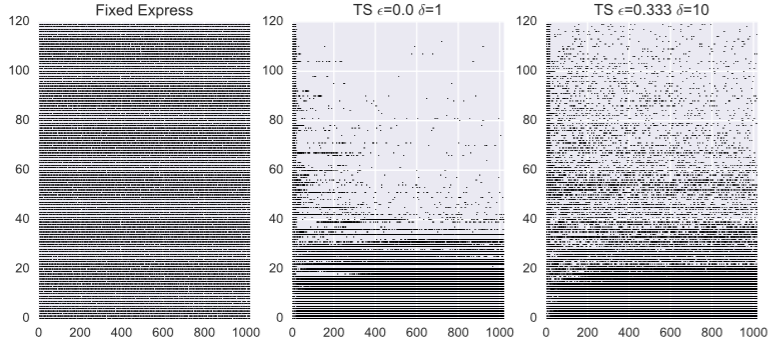
\includegraphics[width=1\textwidth]{plots/3dotplot-lowres.png}
\label{fig:dots}
\end{figure}


\subsubsection{Exploration-diffuse and Bayesian Bootstrapping}

To implement \edts, much like any TS-based algorithm we consider, the researcher must choose between alternative computational approaches for characterizing asymptotic point estimate distribution and Bayesian Bootstrapping. 

We consider Laplace Approximation to the posterior, using mean and asymptotic variance-covariance of the asymptotic multivariate normal distribution. Here, we let $\delta_p$ be a variation inflation factor directly applied to the estimates as, $\delta_p  \hat \sigma$, ($\delta_p \geq 1$), where higher values force more sampling uncertainty.

However, instead of making the distributional assumptions in the asymptotic approach, we consider Bayesian Bootstrapping. We let $\delta$ be the percentage of data to be used for the bootstrapped subsample size, indirectly inflating the estimator's variance. In the Bayesian Bootstrap case, the lower values in $0 < \delta \leq 1$ lead to more uncertainty in the estimate across bootstrapped samples.

Figure \ref{fig:illustrating_edts} illustrates how \edts differs from TS. We sample only 15 of the 20 items dictated by standard TS ($\numperset=20$, $\epsilon=1/4$). The remaining 5 of 20 items are drawn using a more diffuse TS approach. Here, we subsample $\delta$=.25 of the data with replacement and draw $u$ as a Bayesian Bootstrap of the subsampled data. 

\begin{figure}
\caption{Shown is an illustration of TS versus \edts for two items (1st, top; 60th, bottom) at two points in time (left, early; right, late). The graphs show the TS and \edts belief distributions and the underlying diffuse distribution in \edts. The distributions are shown for early beliefs after respondent 40 (left column of plots) and late beliefs after respondent 500 (right).}
\label{fig:illustrating_edts}
 	\begin{center}
    \subfloat[Early, 1st rank]{{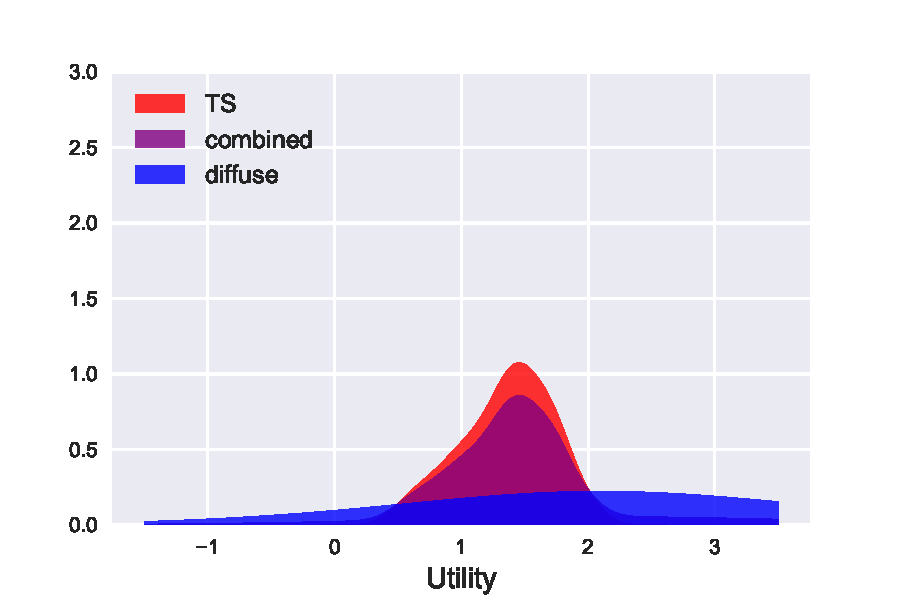
\includegraphics[width=.4\textwidth]{plots/utildifdis600.pdf} }}%
    \qquad
    \subfloat[Late, 1st rank]{{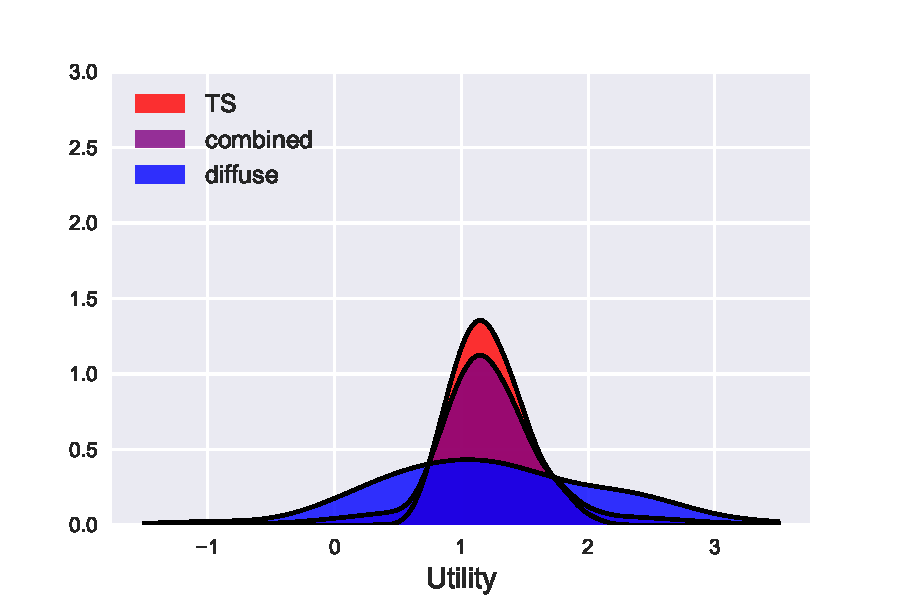
\includegraphics[width=.4\textwidth]{plots/utildifdis3000.pdf} }}%
    \qquad
    \subfloat[Early, 60th rank]{{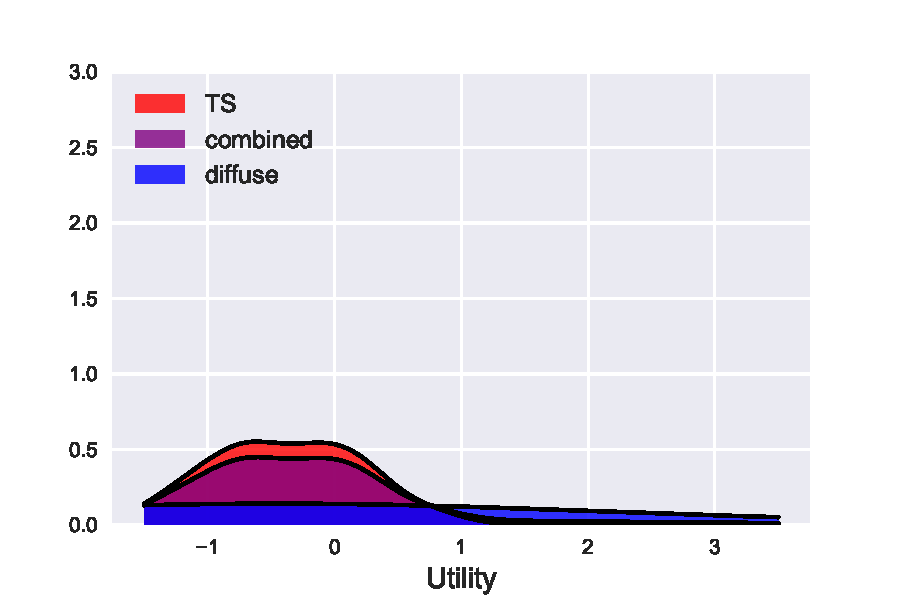
\includegraphics[width=.4\textwidth]{plots/utildifdis6060.pdf} }}%
    \qquad
    \subfloat[Late, 60th rank]{{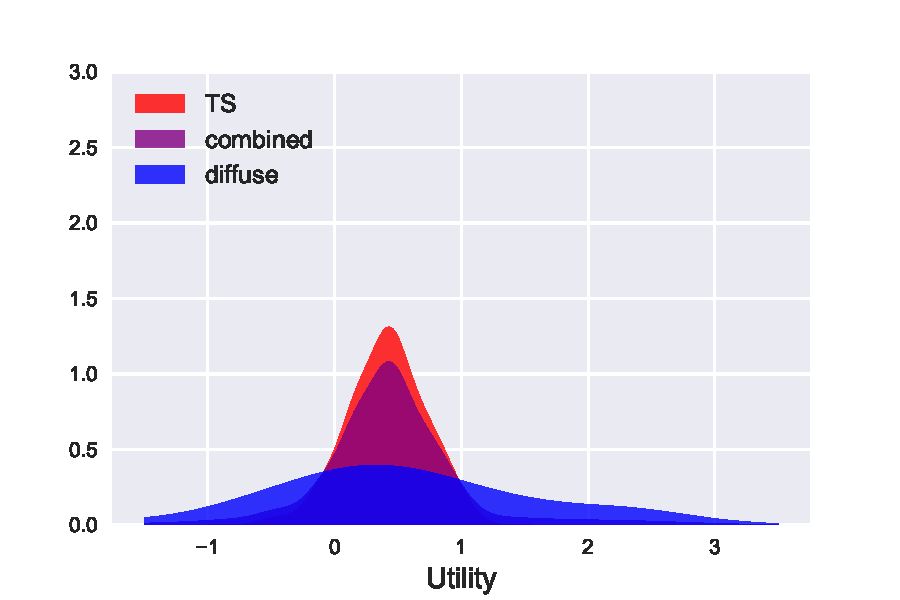
\includegraphics[width=.4\textwidth]{plots/utildifdis30060.pdf} }}%
    \end{center}
\end{figure}

For the $\epsilon$-$\delta$ case, density does not spike as quickly. Speed is controlled through two parameters: the proportion of items sampled from the diffuse distribution ($\epsilon$) and a factor increasing variance for the diffuse distribution ($\delta$). As $\epsilon$ increases and $\delta$ decreases, the algorithm slows and explores more to settle on its set of items. 

We show how \edts performance varies with different $\epsilon$ and $\delta$ values in Section \ref{sec:empirical_main}.  For our empirical analysis, we use ($\epsilon=\frac{1}{4}$, $\delta=\frac{1}{4}$). We also test ($\epsilon=\frac{1}{2}$, $\delta=\frac{1}{4}$) and ($\epsilon=1$, $\delta=\frac{1}{4}$), which perform on par with ($\epsilon=\frac{1}{4}$, $\delta=\frac{1}{4}$). Our recommended ranges for the parameters are $\frac{1}{5}\leq \epsilon \leq \frac{1}{2}$, $\frac{1}{4}\leq \delta \leq \frac{1}{2}$.

% \begin{figure}[!ht]
% \caption{Selecting your $\epsilon$-$\delta$ values. 
% 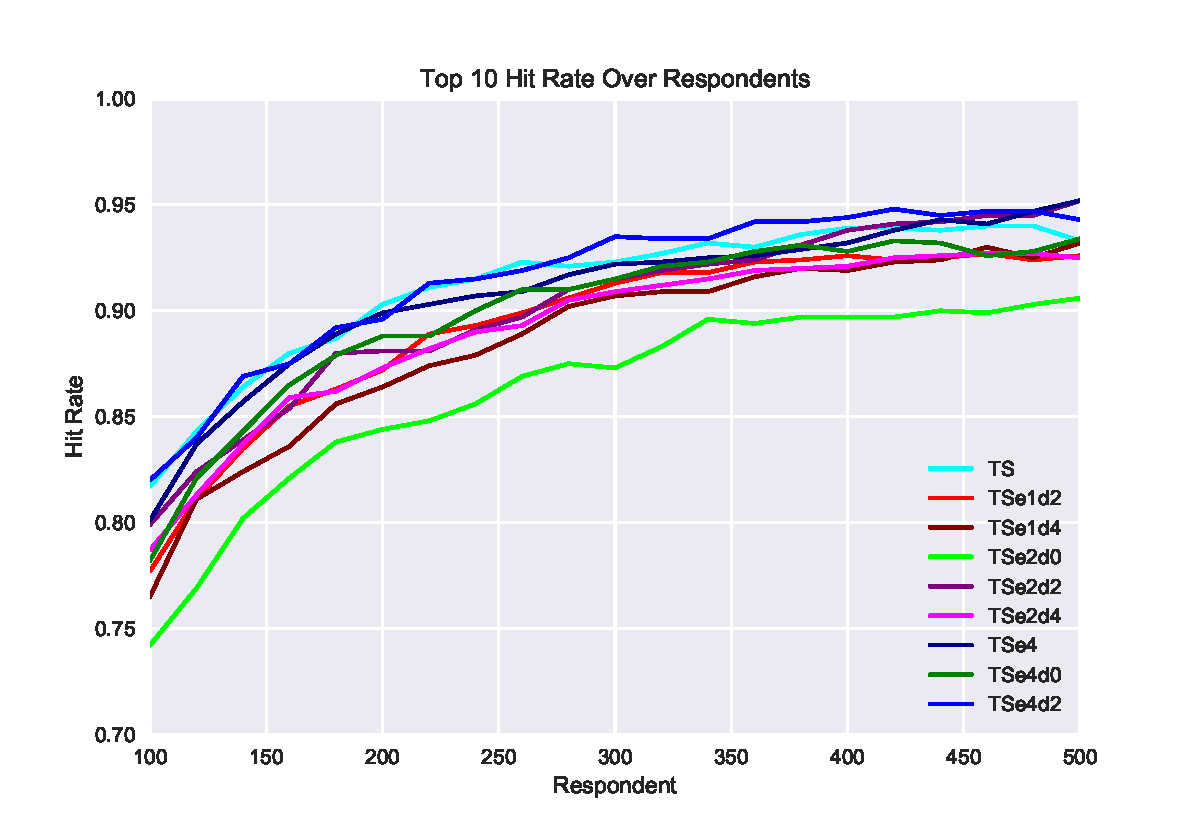
\includegraphics[width=1\textwidth]{plots/hr120v20k10ed.pdf}
% \label{fig:ed}
% \end{figure}

\subsubsection{Exploration Diffuse with Threshold}

To define an exploration-diffuse TS version with a threshold (\edtsthres), we begin with two draws: $u_R$ from the standard posterior and $u_D$ from the diffuse posterior. We calculate threshold-based item scores $s_R$ and $s_D$ for each and take $(1- \epsilon) \numperset$ items with the best $s_R$ scores and $\epsilon \numperset$ items, with the best $s_D$ scores not already included. 

As \edts nests $\epsilon$-greedy sampling, \edtsthres encompass $\epsilon$-greedy. We use the scores $s_i=|u_i - |$ for $c=\frac{u_k+u_{k+1}}{2}$ and take the $((1-\epsilon)L)$ best but sample the remaining scores uniformly (i.e., the most diffuse distribution).


The intuition behind thresholding is best visualized in Figure \ref{fig:Frequency}, which shows how \edts focuses on the top items and \edtsthres provides more of a spread and focuses on items near the decision boundary, in this case the top 20 items. 
\begin{figure}%
    \caption{The frequency of the selected survey item is shown for \edts and \edtsthres.}%
    \label{fig:Frequency}%
 	\begin{center}
    \subfloat[]{{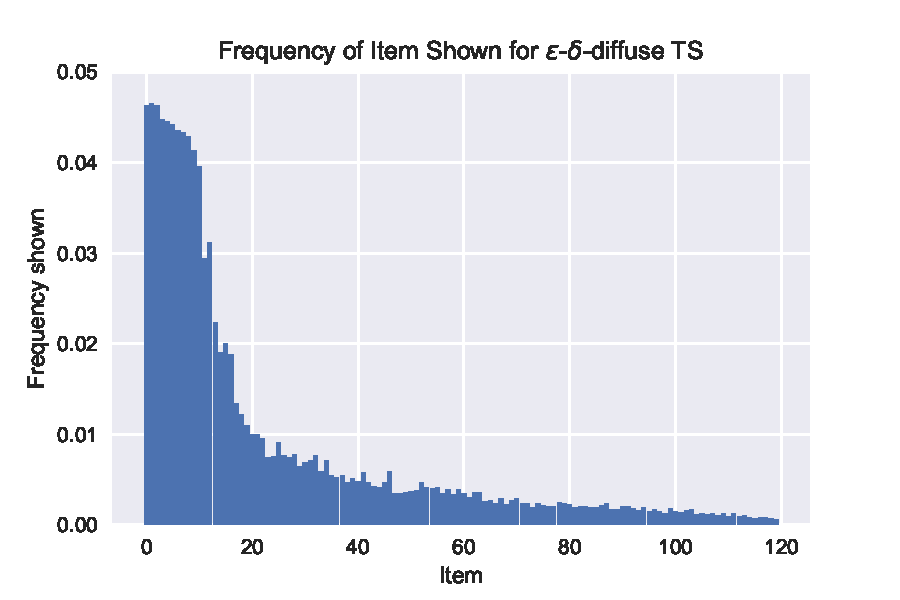
\includegraphics[width=.8\textwidth]{plots/edTSfreq.pdf} }}%
    \qquad
    \subfloat[]{{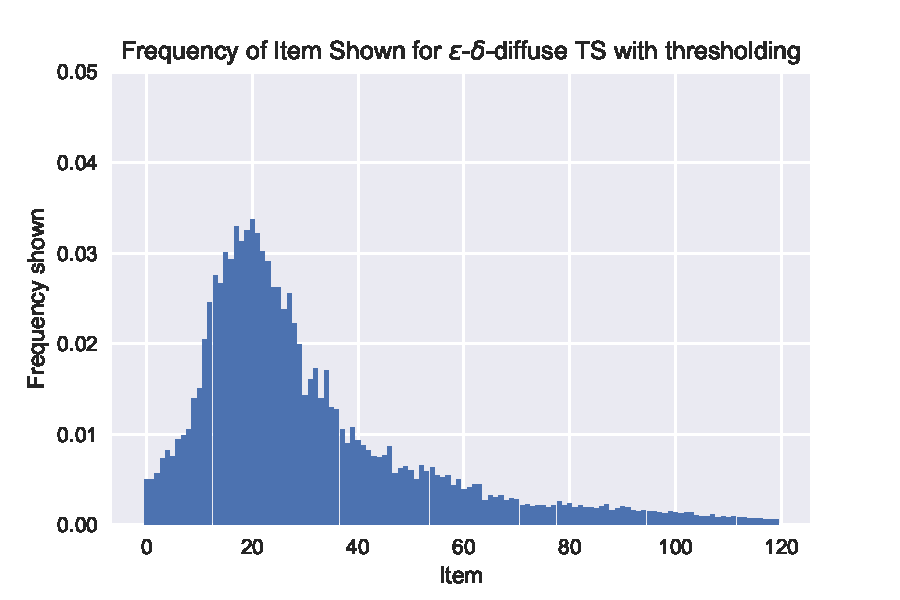
\includegraphics[width=.8\textwidth]{plots/edTSthresfreq.pdf} }}%
	\end{center}
\end{figure}

%Imagine showing three items out of six (A, B, C, D, E, and F) to a respondent. We want to identify the top three items. Let A, B, C, D, E, and F be the utility order. We are certain A and B are in the top three, and E and F are not. An algorithm without thresholding would pick A, B, and either C or D. A will be chosen as the best item, and C or D will be chosen as the worst, giving us no new information. An algorithm with thresholding will pick C, D, and either B or E. In either case, the respondent will be forced to compare C and D, providing information about which is in the top three.



\section{Bandit MaxDiff}

Now we instantiate the general set of algorithms in the particular setting of applying the propose algorithms -- inspired by bandits and active learning -- to develop a better procedure for adaptive MaxDiff. First, we formally review MaxDiff, and then integrate the newly proposed methods based on Thompson Sampling.


\section{Preference Measurement}
\subsection{Idea Screening and MaxDiff Scaling}
\begin{figure}
\caption{MaxDiff has become more popular over time with data analysis software users} \label{fig:pop}
\begin{center}
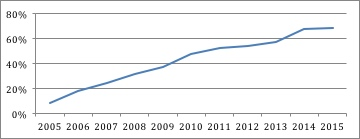
\includegraphics[width=0.5\textwidth]{plots/maxdiffpop}
\end{center}
\end{figure}
MaxDiff is a preference measurement and characteristic scaling method. In a MaxDiff questionnaire, the researcher asks respondents for their most and least preferred items out of a set and repeats the choice task for subsequent sets. Initially proposed by~\cite{louviere1991best}, MaxDiff was first released as a software system in 2004 by Sawtooth Software. Since its release, its popularity has increased steadily, and the technique was used by more than 70\% of Sawtooth Software users in 2017 (Figure \ref{fig:pop}). These users are practitioners of marketing research and consumer insights across industries.

The MaxDiff approach provides more discrimination among items and respondents than traditional rating scales \citep{cohen2004s}. It also avoids the scale-use bias common to traditional ratings techniques \citep{marley2005some,chrzan2006empirical}.

The MaxDiff technique is closely related to conjoint analysis, but MaxDiff allows the respondent to select a best and worst item instead of only one, which is what makes it best-worst scaling \citep{marley2005some}. In its most common form, MaxDiff may be thought of as a one-attribute, choice-based conjoint study with many levels. But MaxDiff can be applied to full-profile multi-attribute alternatives as well \citep{marley2012models}. The differences between conjoint and MaxDiff in their static form are not as relevant for large-scale ranking and selection problems as the differences between the adaptive versions, as the adaptive conjoint objective differs from our objective.

\subsection{Studying Many Items with MaxDiff}

Market researchers used MaxDiff for analyzing large numbers of possible consumer preferences, and the definition of ``large'' has changed in recent years. \cite{hendrix2007alternative} describe ``large sets'' as about 40 to 60 items, proposing MaxDiff variants Augmented and Tailored MaxDiff to handle them. \cite{wirth2012largeset} also investigated MaxDiff variants, Express and Sparse MaxDiff, for handling ``very large sets'' of more than 100 items. The researchers conduct a simulation study of robotic respondents using 120 items and a real study among consumer respondents with 60 items. In this paper, we refer to even larger numbers of survey items, at least 100 items and potentially 300 or more. Our goal is to explore how algorithms scale and how market researchers can push MaxDiff further than ever before.

A 2015 Sawtooth Software customer feedback survey revealed users' need to accommodate more consumer preference items (see Appendix, Figure \ref{fig:max_and_purpose}). Nearly 20\% of respondents indicated their firms had conducted a study with more than 50 items; the maximum was 400. However, according to Sawtooth Software guidance for typical problems, the recommended number of items for a MaxDiff study is about 30, and the alternative profiles recommended for a conjoint study is about 20. The respondents were also asked the main purpose for their large-scale MaxDiff studies. For 42\% of the studies, the main purpose was to identify the top or top few items. Our research shows that for such settings, traditional design strategies can be wasteful, and an adaptive approach can save firms time and money.


% One setting where practitioners consider MaxDiff studies with more than 50 or even 400 distinct product features or service characteristics is the way those items are defined. Those MaxDiff items may represent conjoined elements, like a combination of packaging style, color, claims, and highlighted ingredients. In addition, profiles involving multiple, highly interactive attributes pose challenges for choice-based conjoint analyses, making large-scale MaxDiff studies viable alternatives.


 % can be up to 4x more efficient-- without the Bandit MaxDiff approach, you are potentially wasting 75 cents of every dollar you are spending on MaxDiff data collection. 

\subsection{MaxDiff: A Best-Worst Scaling Choice Model}

In a standard MaxDiff study, every respondent selects both the best and worst option from an available set of characteristics in each discrete choice task. The model for the data comes from a class known as best-worst scaling, one of which is MaxDiff. We adopt our framework from the best-worst scaling literature \citep{marley2005some,marley2012models}. 

Suppose we a set, $S$, for each choice task. Then we can define two random variables: best ($B_z$) and worst ($W_z$) for each $z \in S$.  We then define a third random variable, best-worst $BW_{r,s}$, for any $r,s \in S$. Following a random utility framework, the utilities have deterministic and stochastic components. Thurstone provides a consistent random utility model where each $\gamma_z$ features the extreme value distribution. Because the model is consistent, we have $B_z=-W_z=U_z$ and $BW_{r,s}=U_r-U_s$ and
\begin{align*}
&B_z=v_z+\gamma_z\\
&W_z=-v_z-\gamma_z\\
&BW_{r,s}=v_r-v_s+\gamma_r-\gamma_s.
\end{align*}We can write the probability an item is the best and worst as
\begin{align*}
&B_S (x)= Pr⁡( B_x=\max_{z \in S} B_z)\\
&W_S (y)= Pr⁡( W_y=\max_{z \in S} W_z).
\end{align*}
Without using the particular utility or item scale, we can derive choice probabilities. In the most general form, we suppose $b()$ and $w()$ are separate interval scales. The resulting probability of an item being best or worst is
\begin{align*}
&B_S (x)= \frac{b(x)}{\sum_{z \in S}b(z)}\\
&W_S (y)= \frac{w(y)}{\sum_{z \in S}w(z)}.
\end{align*}
For any pair of items $x,y \in S$, we can indicate the joint probability that $x$ is best and $y$ is worst. However, when considering best and worst together, the scales $b$ and $w$ are not separately identified. We fix their ratio for the same item by setting $w(z)=\frac{c}{b(z)}$. The resulting joint probability is a function of the scale ratios for pairs: 
\begin{align*}
&BW_S(x,y)=Pr(U_x>U_z>U_y | z \in S -\{x,y\}, x\neq y)\\
&BW_S(x,y)=\frac{b(x)/b(y)}{\sum_{r,s \in S, r \neq s}b(r)/b(s)}.
\end{align*}
To accommodate the standard utility structure, we let utility $u(z)=\log{(b(z))}$, making each of the probabilities 
\begin{align*}
&B_S(x)=\frac{e^{u(x)}}{\sum_{z \in S} e^{u(z)}}\\
&W_S(y)=\frac{e^{u(y)}}{\sum_{z \in S} e^{u(z)}}\\
&WB_S(x,y)=\frac{e^{u(x)-u(y)}}{\sum_{r,s \in S, r\neq s} e^{u(r)-u(s)}}.
\end{align*}
We can derive the same representation from the random utility model suggested by \cite{marley2005some}. We can view best-worst choice as a generalization of the classic multinomial logit technique for selecting best only.

\subsubsection{Best-Worst Model Estimation}

One way to estimate the MaxDiff choice model is to enumerate all possible pairs of items and describe the joint probability of being best and worst. This is the probability of yielding the largest difference $BW_S(x,y)$ in consumer behavior. This pairwise approach is not practical because it scales quadratically for number of items. So, we adopt an alternative approach reflecting the literature and practice that is shown to be a near exact approximation of the full model \cite{cohen2003maximum}. This allows us to estimate the best model and worst model independently, without explicitly estimating the best-worst probability. (See Appendix for details.)

%\textbf{Emphasize our goal is to identify the top items.}

\section{Bandit MaxDiff}

%We utilize the best available bandit alogrithms and draw upon the active learning and best k arm identification problems. Thompson Sampling involves allocating resources to an action in proportion to the probability that it is the best action~\cite{thompson1933likelihood}. 

Our proposed approach, Bandit MaxDiff, incorporates adaptive learning as a natural method for solving top-set ranking and selection problems. Our approach leverages prior learning during survey administration to create more efficient questionnaires and more precise aggregate score estimates. On the one hand, we want to come to a conclusion about the relative importance of a large number of product or service characteristics within a MaxDiff problem. On the other hand, we want to utilize what we have learned as we go to target actions likely to allow the researcher greater precision. TS has proven useful for these types of problems \citep{schwartzetal2017,russo2017tutorial}.

For each of our survey respondents, we select $\numperset$ items and generate a MaxDiff design of $J$ best-worst tasks, each with a choice set of $|S|$ items. For example, as our empirical default, we use $\numperset=20$, $J=12$, and $|S|=5$, standard numbers used in MaxDiff studies \citep{wirth2012largeset}. 

We begin as in a traditional MaxDiff design, showing each item an equal number of times across all respondents and tasks to ensure a balanced design.  For the first respondent, we select the $\numperset$ items uniformly. 

After the initial respondent batch, we remain uncertain about each item's parameter value, so we continue collecting data. But we do not need to reduce uncertainty equally, so we adapt strategically. At each subsequent period after collecting a set amount of respondent data, we estimate a model to characterize our parameter beliefs. We systematically oversample the items already viewed as most preferred, the top set. But we also recognize our uncertainty about the top-set items. Figure \ref{fig:dots} shows the oversampling as data accumulate. As the sample size increases, uncertainty around which items are best tightens.


Bandit MaxDiff uniquely translates our current beliefs about parameters into decisions about what to ask subsequent respondents via oversampling the best items in a principled manner. The approach is summarized in Table \ref{methods}.

\begin{algorithm}
\caption{Bandit MaxDiff: \ts} \label{alg:ts_simple}
\begin{algorithmic}[1]
\State Given: $K,\numperset,J,S,b$.
\State Initialize first set of questions by sampling $\numperset$ items uniformly.
\State Design MaxDiff questionnaire covering $\numperset$ items with $J$ tasks of $S$ questions each, $\text{MDDesign}($\numperset$,S,J)$, for the next batch of $b$ respondents.
\State Collect new data from respondents with $n = b*t$ respondents.
\State Bayesian Bootstrap sample weight replacement using weights ($\alpha_1, ...., \alpha_n)\sim \text{expon}(1)$, obtaining some subset of $n$ previous respondents.
\State Estimate model parameters ($\theta_t$) and obtain estimated utilities $u = (u_1,...,u_K)$.
\State Choose $\numperset$ items using draws from empirical posterior.
\State Select next questions for respondents.
\end{algorithmic}
\end{algorithm}
% $S=\#\{\mathcal{S}\}$



\subsection{Bandit MaxDiff and Posterior Sampling} \label{sec:bmd_ts_edts}

The Bandit MaxDiff base algorithm draws on TS to address the multi-armed bandit problem. The method's specific instantiation is shown in Algorithm \ref{alg:ts_simple}.
  
\subsubsection{Learning with Bayesian Bootstrapping}

For TS models, we first characterize parameter uncertainty. We use a multinomial logit model; the first but least practical option to obtain posterior draws would be to use the Markov Chain Monte Carlo, which would be too slow to update in real time. A more practical way to approximate the posterior is to sample from the asymptotic distribution via the maximum likelihood implied by the estimated mean and standard errors, a Laplace Approximation of the Posterior \citep{tierney1986accurate}. The Laplace approach reflects the estimated population preferences and normally distributed error, with standard deviations equal to the standard errors of the parameter estimates. The method would work quickly, but it forces the joint posterior into a multivariate normal distribution. 

We can obtain posterior samples using the Bayesian Bootstrap method by sampling weights $\beta$ for each respondent: $\beta_1,\beta_2,\ldots,\beta_N \sim \text{exp}(1)$. The weights are used for sampling respondents with replacements to form a new bootstrapped dataset. If a respondent is sampled, all the data is included in the bootstrapped sample. The probability of any one respondent $i$'s data being sampled in any one draw is $\beta_i / \sum_{i}^{N}\beta_i$.  For each bootstrapped dataset, we obtain parameter estimates of $\theta$ using a weighted  maximum likelihood estimate as follows:
\begin{align}
&LL(\theta;\beta)=\sum_{n=1}^N \beta_n
\sum_{x \in S_n} 
	\left(
		Y_{B_{S_n}}(x)
		\log{\frac{e^{\theta_x}}{\sum_{z\in S_n} e^{\theta_z}}} 
		+ 
		Y_{W_{S_n}}(x)
		\log{\frac{e^{-\theta_x}}{\sum_{z\in S_n} e^{-\theta_z}}}
	\right) \\
&\theta^\beta = \text{arg}\max_{\theta} LL(\theta;\beta) ,
\end{align}

where each estimate $\theta^\beta = u_1^\beta, \ldots, u_K^\beta$ implies a rank ordering of all items $\pi_{u}^{\theta^\beta} = \pi(1),\ldots,\pi(\numperset),\pi(\numperset+1),\ldots,\pi(K)$. The items corresponding to $\pi(1),\ldots,\pi(\numperset)$ form the next list of $\numperset$ items to show the next respondent. 

While the Bayesian Bootstrap is rarely used for posterior sampling, we use it throughout our empirical application because of its conceptual appeal and speed. Because we only need one set of $\numperset$ items per respondent, we can obtain new bootstrapped samples $\theta^{\beta}$ and $\pi(u|\theta^\beta)$ for each new respondent. If we seek the probabilities with which any item would be selected, we can obtain many independent and parallelized samples. 

\subsubsection{Bandit MaxDiff and \ts Intuition }

While collecting data for the Bandit MaxDiff algorithm, imagine we have 100 respondents and can summarize the population's preferences for 300 characteristics, with their item-specific parameter values in a multinomial logit model. To generate a MaxDiff task for the 101st respondent, we draw from the population preferences, leveraging mean estimates and normal errors with standard deviations equal to the standard errors' point estimates. We sort the newly sampled vector of preference values from the most to least preferred item. The most preferred can be used to create the sequence of MaxDiff choice tasks for the 101st respondent.

A typical bandit algorithm is not practical here. While selecting an arm means including an item in the survey for the next respondent, the reward is not revealed each period. Since each respondent must see only a subset of items, the item receiving the ``best'' label in a choice task does not translate directly to a reward. The choice data allows us to infer how each item ranks among all characteristics, aligning with our managerial goal.

The posterior variation---the sample-to-sample differences in parameter value and relative rank ordering---is critical. Even when little data has been collected, we have substantial uncertainty. The independent samples differ in rank order of item utilities. This allows MaxDiff designs across respondents with less overlap in items. Later, uncertainty is reduced most around the truly high-utility items. Across independent samples, item ranking is highly correlated near the top but not near the bottom, where uncertainty remains. As a result, the top subset of $\numperset$ items selected converges to the same group for each respondent. The algorithm learns over time, identifying items with truly high utility with high precision (Figure \ref{fig:illustrate_ts}). 

\begin{figure}
\caption{Shown is an illustration of a MaxDiff Thompson Sampling procedure.}
\label{fig:illustrate_ts}
	\begin{center}
    \subfloat[Early]{{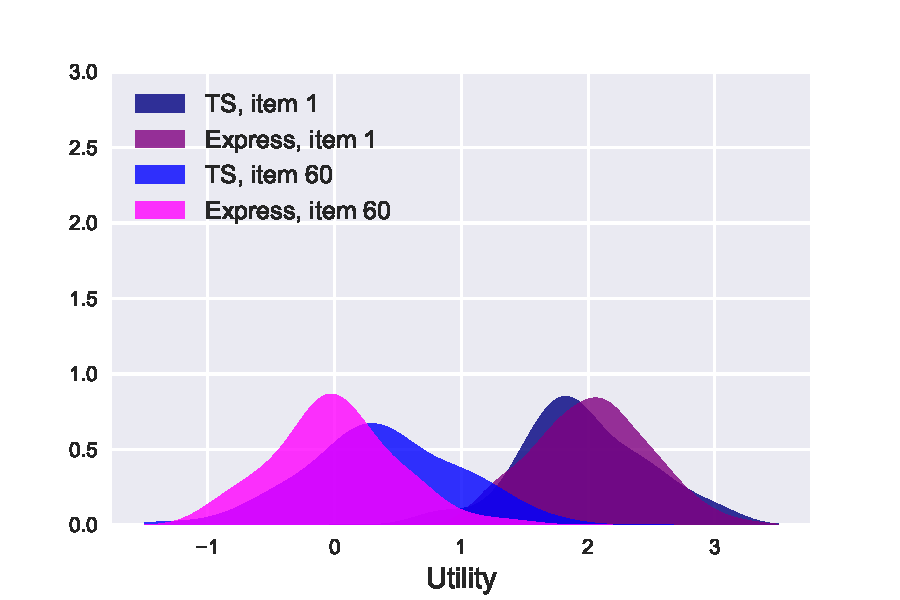
\includegraphics[width=.4\textwidth]{plots/utildis60.pdf} }}%
    \qquad
    \subfloat[Late]{{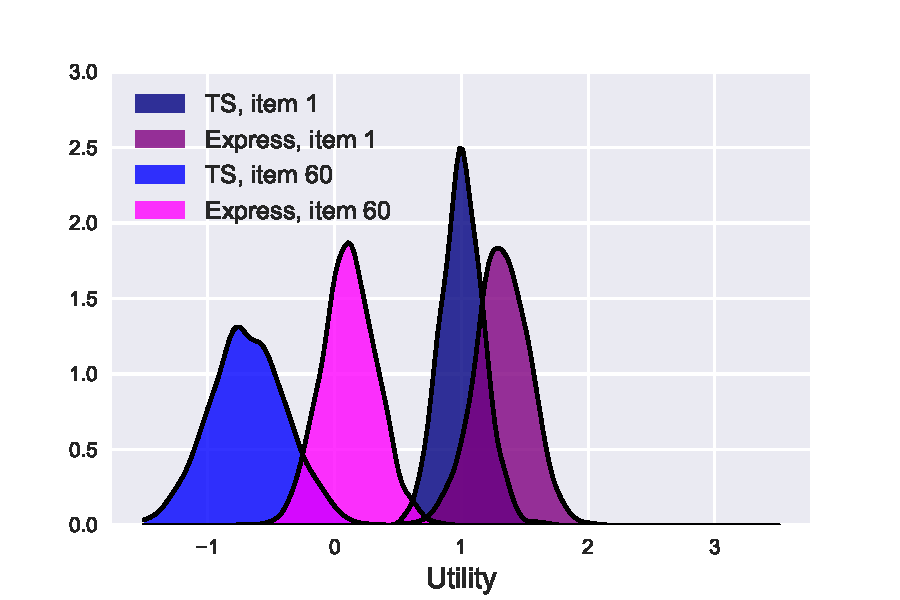
\includegraphics[width=.4\textwidth]{plots/utildis300.pdf} }}%
    \end{center}
\end{figure}

\subsection{Exploration-diffuse Thompson Sampling}

Changes over time can cause robustness issues for TS algorithms. On the one hand, TS features built-in robustness---the algorithm is stochastic and adapts continuously. If early survey data leads the algorithm astray, it will self-correct, eventually finding and converging on the respondents' most preferred items. 

Suppose  early respondents make choices leading the researchers to believe certain survey items are best when they are not. Subsequent respondents will then be shown the items, and uncertainty will be reduced, indicating other items are likely better. By sampling from the item utilities' joint belief distribution, we will be less likely to draw the items which will eventually be shown as poor performers. 

Such sampling could be too aggressive, as the natural parameter uncertainty is not sufficient. Or it may be too slow to adjust to large changes in the sampled respondents, reflecting either a shift in the population or that the earlier respondents are not representative of the broader population. This potential problem can be addressed with \edts.


\begin{table}
\begin{tabular}{p{3in}|p{3in}}
Algorithm & Description of sampling scheme \\
\hline
MaxDiff TS & Take $\numperset$ items with highest utility sampled from the posterior.\\
MaxDiff $\epsilon$-Diffuse TS & Take $(1-\epsilon)L$ items with highest utility sampled from the regular posterior; sample from diffuse posterior distribution, and take $\epsilon L$ items with highest sampled utility from remaining items.\\
$\epsilon$-Greedy & Take $(1-\epsilon)L$ with greatest current estimated $\theta$; take remaining $\epsilon L$ uniformly from remaining items.\\
TS Closest to the Threshold & Take $\numperset$ items with sampled utility closest to $\frac{u_k+u_{k+1}}{2}$.\\
$\epsilon$-Diffuse TS Closest to the Threshold & Take $(1-\epsilon)L$ (from posterior) and  $\epsilon L$ (from diffuse posterior) items with sampled utility closest to $\frac{u_k+u_{k+1}}{2}$.\\
$\epsilon$-Greedy Closest to the Threshold & Take $(1-\epsilon)L$ items with estimated utility closest to $\frac{\theta_k+\theta_{k+1}}{2}$ and $\epsilon L$ items uniformly from remaining.\\
Misclassification Minimization with Random Perturbation& Take $\numperset$ items most likely misclassified (bottom items that should be top and vice-versa); add perturbation to probability.\\
Greatest Uncertainty with Random Perturbation& Take $\numperset$ items with probabilities of being top at closest to 50\%; add perturbation to probability.\\
\end{tabular}
\caption{Summary of Adaptive MaxDiff Algorithms.}\label{methods}
\end{table}

% \textbf{Shea: Make captions for all tables flush left}

%%Discuss relation to the Follow the regularized leader / perturbed leader 

% \subsection{BAM for Best-Arm Identification}

% \subsubsection{New Variant: Closest to the Threshold}

% \begin{verbatim}
%        utilities        rank ordering
% item : a b c d e f   max(1)(2)(3)(4)(5)(6)min
% draw1: 6 7 7 8 8 9  -->  f  d  e  c  b  a   
% draw2: 7 5 5 9 8 6  -->  d  e  a  f  b  c 
% draw3: 6 4 5 8 7 5  -->  d  e  a  c  f  b 
% \end{verbatim}

% \subsubsection{Algorithm Misclassification Minimization}

\subsubsection{Uniform Sampling: Fixed Express MaxDiff}
We uniformly and randomly draw $\numperset$ of $K$ items without replacement to show to each respondent, achieving balance across items and respondents. For example, in a problem with $\numperset=20$ of $K=120$, each item appears $\frac{J*S}{L} = \frac{12*5}{20} = 3$ times per respondent on average.

\subsubsection{$\epsilon$-Greedy}
We test $\epsilon$-greedy as a baseline for our adaptive methods, letting $\theta$ be the current estimated parameters. We take the $(1-\epsilon)L$ items with the greatest $\theta$ value and choose the remaining $\epsilon L$ uniformly. We use $\epsilon=\frac{1}{4}$ for our empirical analysis and test others. For greedy alone, $\epsilon=0$ would always serve the top $\numperset$ items with the highest estimated average utility to subsequent survey respondents.






\section{Empirical Analysis: Main Results for Bandit MaxDiff}

\label{sec:empirical_main}
We compare our proposed set of adaptive approaches to existing adaptive and non-adaptive strategies. We use simulated choice data based on inferred preferences from an actual MaxDiff survey.

\subsection{Simulation Experiment Setup}

\subsubsection{Data Generating Process}

Our dataset, consisting of 981 respondents and 120 items, comes from a survey conducted by P\&G using Sawtooth Software. The items represent product features and benefits, but the subject matter and item text is hidden for confidentiality purposes. The questions come from a sparse MaxDiff study using a fixed, non-adaptive design with balance across all items and respondents. 

Instead of raw choice data, we have the individual-level posterior mean utilities for all respondents and items, which are obtained via Markov Chain Monte Carlo sampling for a hierarchical Bayes logit model. We call these individual-level mean utilities the ``truth'' in our data-generating process. The utilities offer realistic preference patterns across the items and respondents and permit us to generate data for our respondent simulations.  Therefore, our simulated respondents mimic the actual respondents' preferences on average---to answer each new MaxDiff task, we perturb those true utilities with independent and identically distributed Gumbel error. 

\subsubsection{Measure of Performance}

After each batch of respondents, we run aggregate logit model to obtain current beliefs of utilities. We compare those current aggregate estimated utilities to the aggregate of the true aggregate-level utilities, which are the item-specific averaged across all true individual-level utilities. For every case, we run the simulations 100 independent times to obtain a distribution of measures. 

Our primary performance measure is \textbf{top $k$ hit rate}: the proportion of items correctly chosen to be into the top set. 
This hit rate is precisely a rescaled and empirical version of the loss function introduced earlier:
\begin{align}
\text{HitRate}(\topset) := \frac{1}{k} \sum_{ \topset^{*}(u) }  1 - \mathbf{1}\{ i \in \topset \},
\end{align} 
that is, the percentage of the truly top-$k$ items that are predicted to be in the top-$k$ set.

That is, we compute the percentage based on the cumulative sum of instances when true top $k$ items that appear in the estimated top $k$ set at each time point. For example, if the estimated scores identify seven of the true top-10 items, irrespective of order, the hit rate for that period is 70\%. 




We consider a range, $k=3,10,20,40$, depending on the simulation setting. Hit rate is a natural consideration in an active learning problem. It evaluates the quality of the adaptive learning procedures with respect to the eventual decision of selection. It reflects how far we are from always selecting the truly best set of arms for all time periods. 

But we clarify that this particular hit rate measure is appropriate if the goal of the business problem is selecting the top set. It does not consider the rank ordering within the top set (as a particular loss function for ranking would). And hit rate also does not explicitly evaluate the accuracy and precision of the estimated utilities compared to the truth, as mean squared error, MSE, would.  For the clarity and space, we do not show multiple performance measures for all simulations; only for some simulations settings later on, we will show performance in terms of alternative measures, including MSE of estimated utilities and estimated sum of utility values of the chosen top set compared to that of the true best set (akin to regret). The former should be preferable to hit rate, if the business problem is concerned with rank ordering within the top set.

For the main simulation environment, we examine true aggregate utilities in Figure \ref{fig:util}. The differences among the top-item utilities make the task of identifying the truly best items quite difficult. With $K=120$ items in the dataset, we observe that the true preferences for approximately the top 15 respondents are within 1.0 on a logit scale in terms of utility. Due to how tightly the top items are clustered, the hit rate measures we employ are highly discriminating between competing methods.

\begin{figure}[!ht]
\caption{The plot shows the rank order and utility values on the logit scale for all 120 items in the survey, highlighting the top 10 (blue) and top three (red) items. The values become the means for the unobserved data-generating process.}
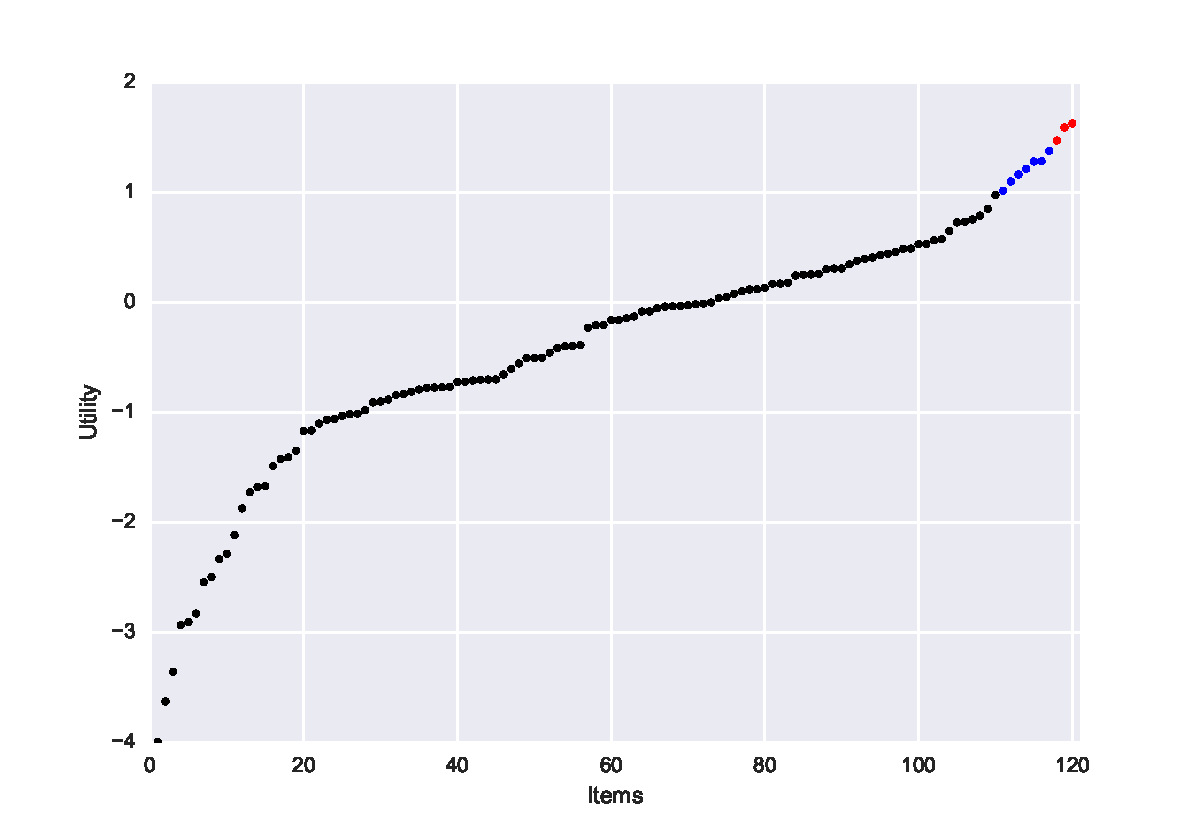
\includegraphics[width=1\textwidth]{plots/utilscore.pdf}
\label{fig:util} 
\end{figure}

\subsubsection{Simulation Experiment Design Factors}


Every setting can be described by a tuple: $\{N,b,K,\numperset,J,S\}$. In the base setting, we simulate the process of collecting survey data about $K-120$ items from $N=500$ respondents in batches of $b=20$ per period. We use bootstrap sampling with replacement from the original dataset of 981 individuals. We consider the first batch of respondents to be initial group, which always receive $\numperset=20$ items uniformly selected, for all methods. In that sense, the adaptive methods only begin after the $20^{th}$ respondent. Each simulated respondent completes $J=12$ choice sets (best-worst tasks), and each set includes $S=5$ items. We then extend the base setting in a variety of dimensions -- $K$, $N$, $\numperset$, $J$ -- and measure performance by varying $k$.

We test the different adaptive approaches found in Table \ref{methods}. For our base setting, we begin use ($\epsilon=\frac{1}{4}$, $\delta=\frac{1}{4}$) for methods involving $\epsilon-\delta$ TS. The natural benchmark common across is existing MaxDiff approach, Fixed Express.


\subsection{Primary Results for Bandit MaxDiff}

\subsubsection{Comparing Fixed Express, Greedy, Thompson Sampling, \edts}

Our primary results highlight that the proposed adaptive methods \ts and \edts, central to Bandit MaxDiff, perform better for large MaxDiff problems than static approaches. But an adaptive greedy algorithm, which does not explicitly incorporate learning, does not perform well enough. Figure \ref{fig:simple_result} shows how \ts improves substantially over the greedy approach, and \edts shows even more improvement for hit rate.

\begin{figure}
\caption{The plots show results for the \fixedexpress, \egreedy, \ts, and \edts algorithms for $\{N=500,b=20,K=120,\numperset=20,J=12,S=5\}$. Performance represents cumulative hit rate per number of respondents at that point in time.}
\label{fig:simple_result}
\begin{center}
	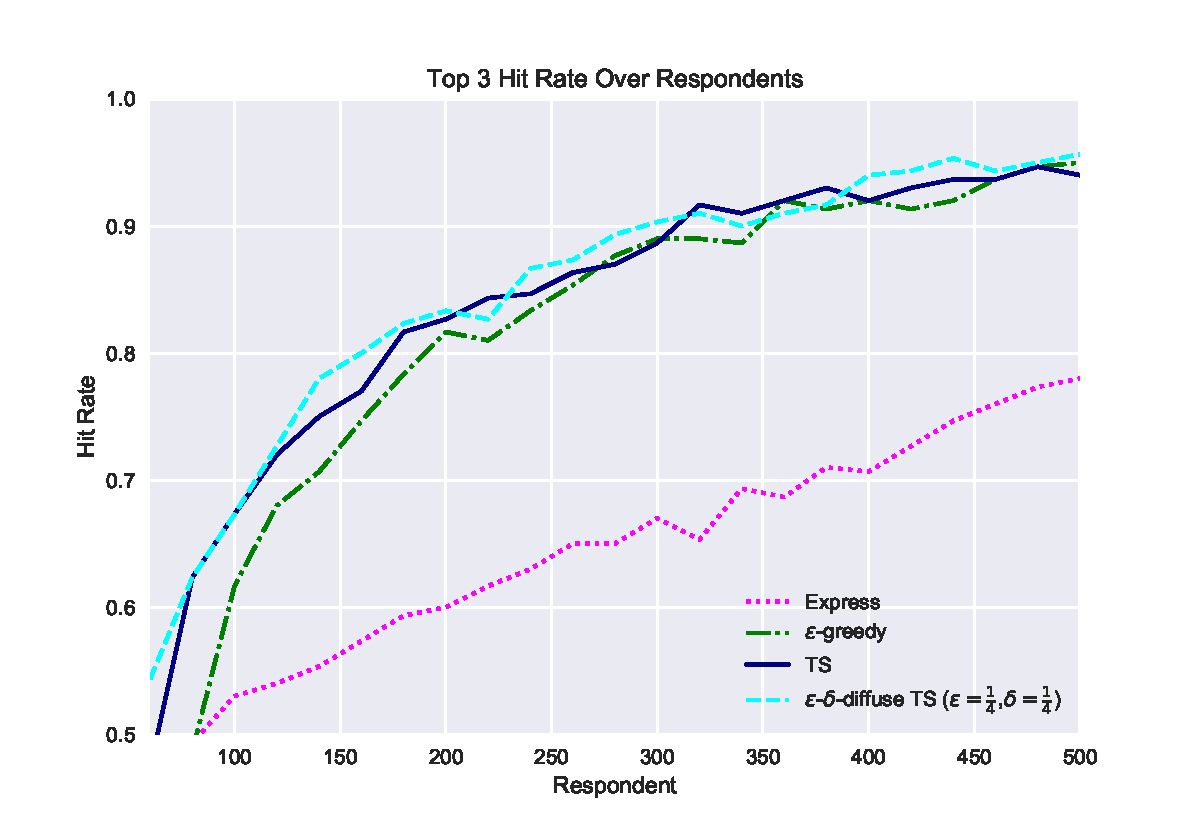
\includegraphics[width=.8\textwidth]{plots/hr120v20k3.pdf}
\end{center}
\end{figure}


Practically speaking the results are significant. If a marketing researcher wants a hit rate of 80\%, the Bandit MaxDiff approach can achieve it \emph{at least three times more efficiently}: using a smaller sample size (about 160 respondents) than the standard Express MaxDiff approach (at least 500 respondents). As we will see the  holds for the different values tested in the basic setting.
 
Viewed another way, we see that after 260 respondents the \ts and \edts have achieved hit rates of about 85\% when standard Express MaxDiff reaches 65\%. As more data are collected, the methods exhibit naturally diminishing returns to scale, as they asymptote close to 100\% hit rate and the non-adaptive approach is still improving. For clarity, to highlight differences, we only show a restricted range: above 50\% hit rate (y-axis) and the first 500 respondents (x-axis), but we the gains continue beyond 2,000 respondents for this problem. The average hit rates for $k=3,10,20,40$, averaged across 100 independent experiments, for this problem are reported in Table \ref{table:at_260_500}.

We now turn to a comparison between the adaptive methods. While \edts slightly outperforms \ts and \egreedy, the gains are mostly earlier on. But we do not mean to overstate those differences in this problem setting. The performance gap between \edts and \ts widens dramatically when considering non-stationary settings, such as a misinformed start (see Section \ref{sec:robust}). 

To better understand, how $\epsilon$ and $\delta$ affect performance of the \edts, we report the results from testing a range of values in Figure \ref{fig:effects_epsilon_delta}. These also display the top $k=10$ hit rate.


\begin{figure}
\caption{The plots show performance with $\epsilon = 1/2$ (left) and $\epsilon = 1/4$ (right), with multiple lines in each plot: $\delta = 1/2$ (dash-dot) and $\delta = 1/4$ (dash). Each of the plots show standard \ts ($\epsilon = 0$, $\delta =1$) performance.}
% Need to remove \delta = 0 from plots.
\label{fig:effects_epsilon_delta}
 	\begin{center}
    \subfloat[$\epsilon=1/2$]{{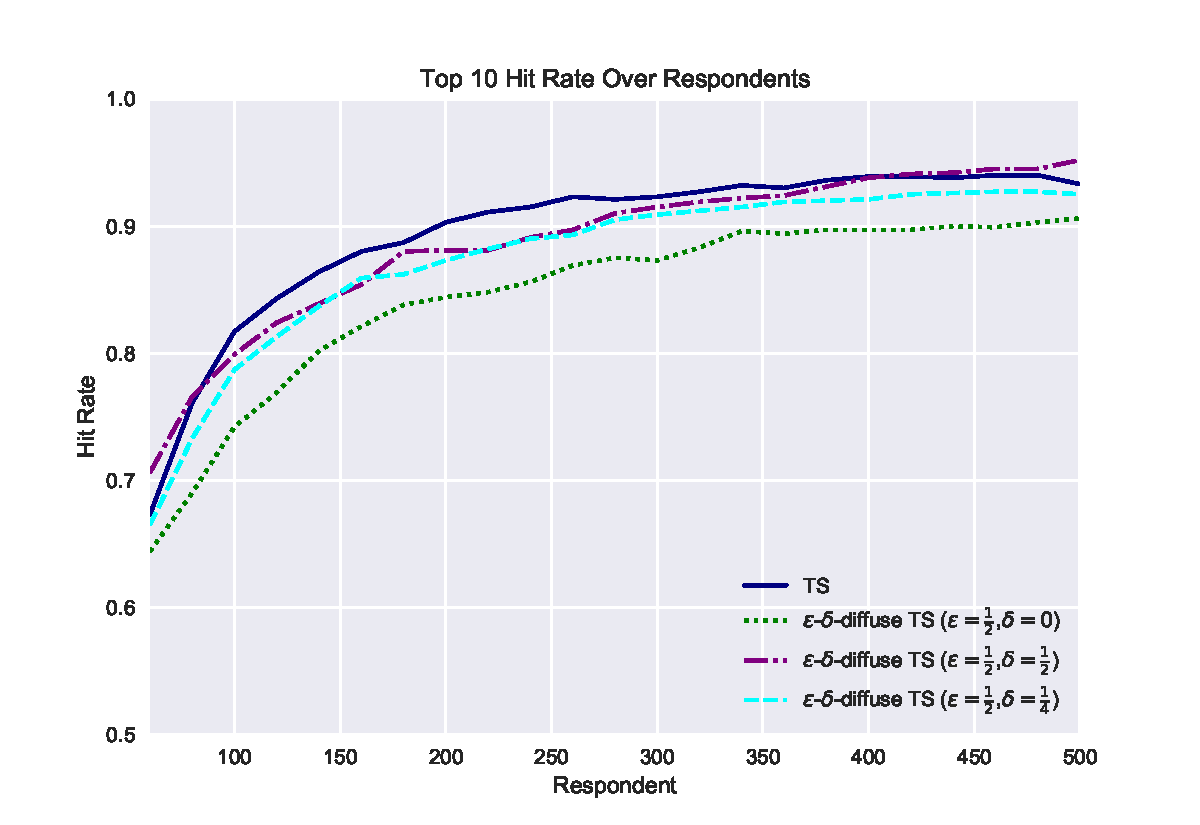
\includegraphics[width=.8\textwidth]{plots/hr120v20k10e2.pdf} }}%
    \qquad
    \subfloat[$\epsilon=1/4$]{{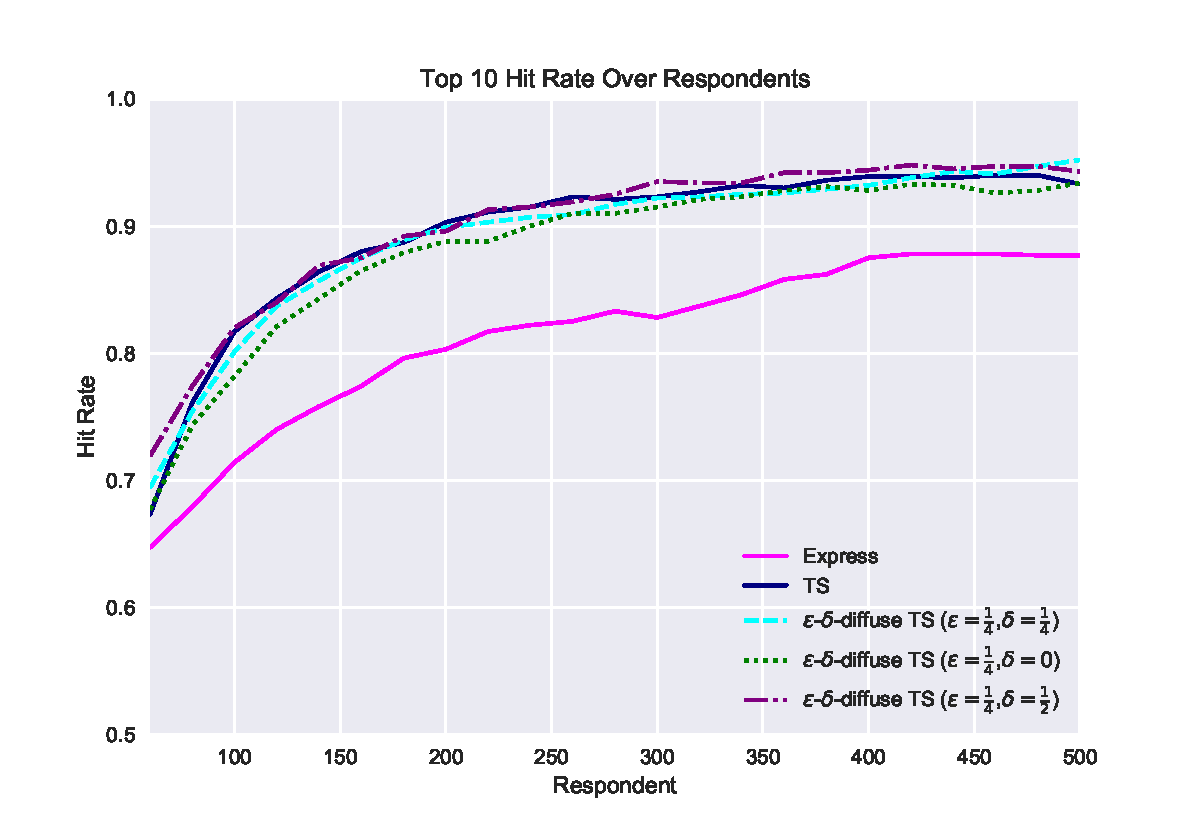
\includegraphics[width=.8\textwidth]{plots/hr120v20k10e4.pdf} }}%
    \end{center}
\end{figure}


\subsection{Focusing Near the Decision Boundary: Thresholding, Uncertainty, and Misclassification}

The intended purpose of all of these was to force sample of items to be near the decision boundary, serving up the $\numperset$ items closest to those with ranks $k$ and $k+1$, instead of focusing on all of the top items ranked $1,\ldots,\numperset$. And a result the percentage of top $k$ items correctly identified would increase since the most precision would be achieved where it mattered most for the decision. 

For the same problem setting as above, $\{N=500,b=20,K=120,\numperset=20,J=12,S=5\}$, we now examine the performance of the active-learning inspired methods that we propose. We devised algorithms \mismin\ and \uncert\ using the same principles and, not surprisingly, they perform similarly well, as seen in Table \ref{table:at_260_500}. But one downside to these two algorithms are their computational cost, obtaining many draws from the posterior at each time step, required to compute the key quantities (e.g., probability of misclassification and probability of being in the top set). 

However, the idea of thresholding can be used in a more computationally efficient manner. The algorithm \edtsthres\ was designed to require only two posterior samples just like \edts.  Figure \ref{fig:threshold_edts_hit10vs20} highlights the impact of adding thresholding to \edts, and indeed it has its desired effect.
\footnote{When we ad thresholding to \ts without the $\epsilon$-$\delta$ diffusion part, the resulting algorithm, \tsthres, does not perform better than its components may suggest. This is because the extra cushion provided by \edts to sometimes sample extreme points is needed to ensure the thresholding is effective.}

\begin{figure}%
    \caption{Adding threshold to \edts}%
    \label{fig:K120_L20_k3hit_k10hit}%
	\begin{center}
	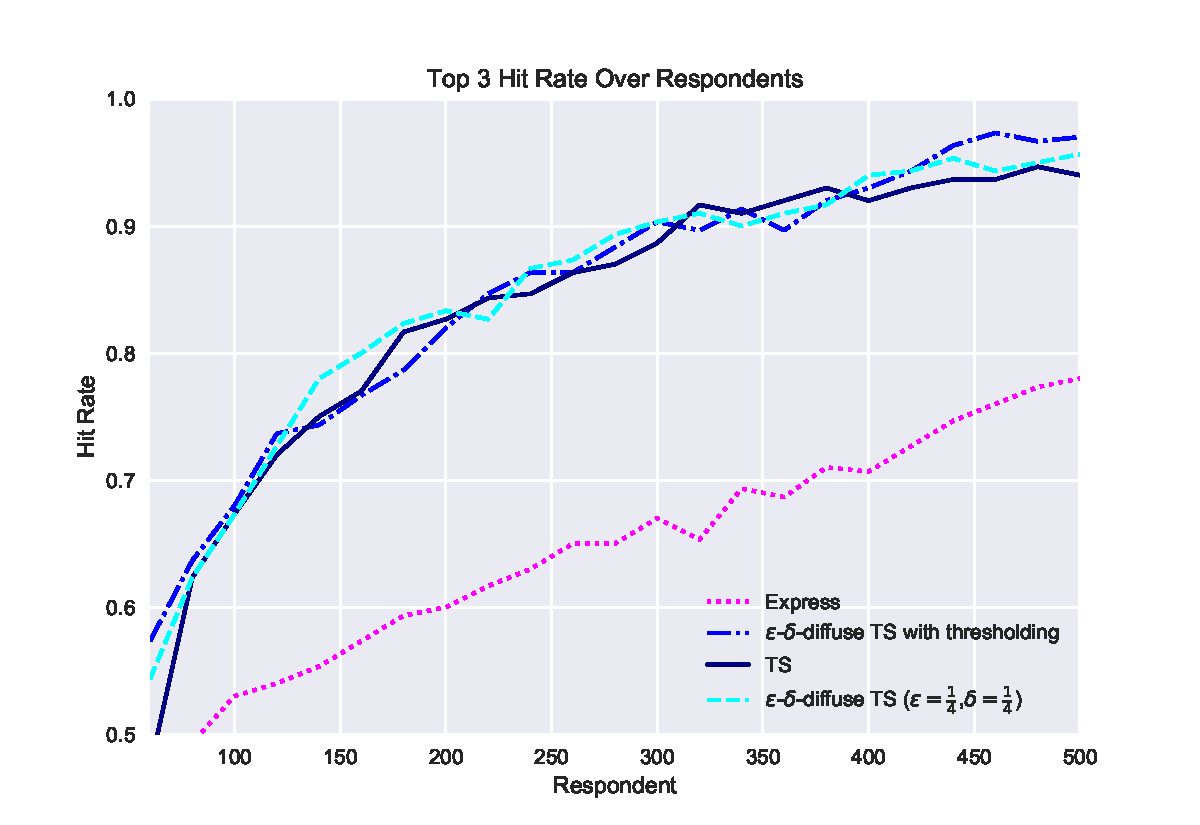
\includegraphics[width=.8\textwidth]{plots/hr120v20k3TS.pdf} 
	\end{center}
\end{figure}

In fact, \edtsthres can serve as a computationally faster -- but equally strong performing -- algorithm compared to the active-learning inspired ones, \mismin and \uncert (Figure \ref{fig:mismin_uncert_thresh_ts_hit10} and Table \ref{table:at_260_500}). We revisit this comparison and the built-in robustness of \edts, when considering the misinformed starts. 

\begin{figure}%
    \caption{Comparing active-learning inspired algorithms (\mismin and \uncert) and thresholding (\edtsthres)}%
    \label{fig:mismin_uncert_thresh_ts_hit10}%
 	\begin{center}
    \subfloat[Top 10]{{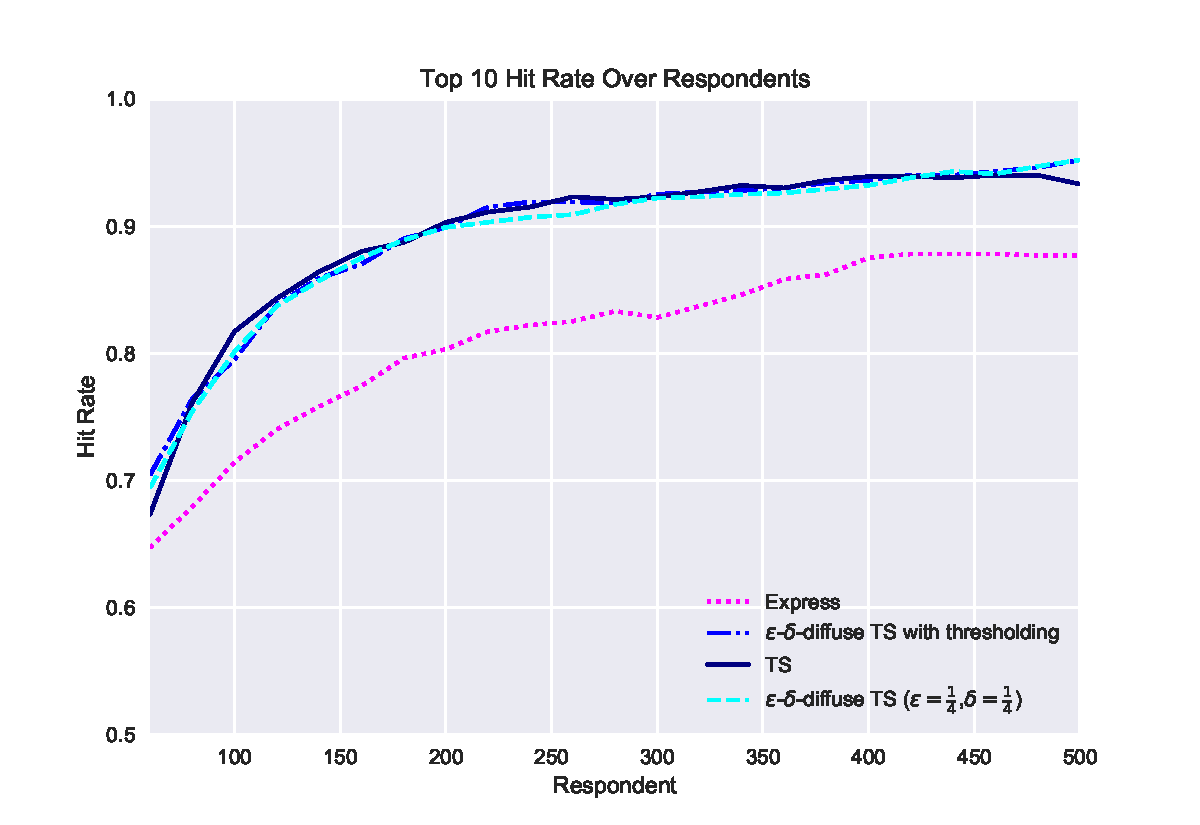
\includegraphics[width=.8\textwidth]{plots/hr120v20k10TS.pdf} }}%
    \qquad
    \subfloat[Top 10]{{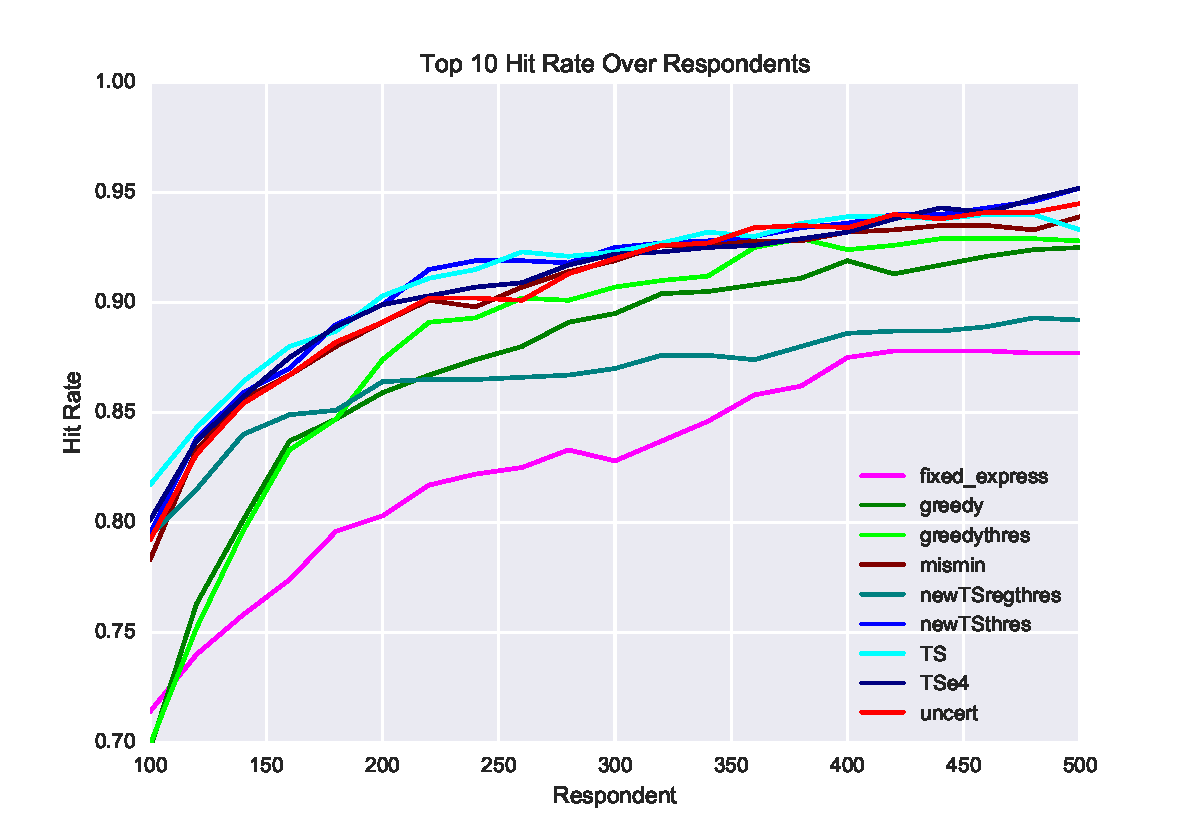
\includegraphics[width=.8\textwidth]{plots/hr120v20k10.pdf} }}%
	\end{center}
\end{figure}



TS alone has its limits---it is constructed to select the best items (and eventually, only the best item), so it performs well identifying a small number of items ($k=3,10$). TS is not suited for the active learning problem, especially when identifying a larger top set, e.g., when a high hit rate for all items in the survey is required ($k=L=20$). While the \edts algorithm adds exploration to improve performance, it does not direct resources toward the areas of high uncertainty at the decision boundary.


We examine hit rate for the top $k$ items, $k = \{3,10,20,40\}$. Smaller $k$ values make the problem more challenging early in the process, as selecting the top three out of 120 is more difficult than selecting the top 40 out of 120, particularly in light of the true utility value distribution (Figure \ref{fig:util}).  

 Table \ref{table:at_260_500} 


 %\eric{Why is \ts better than \tsthres for $k=10$?   }


%For top $k=20$ with 120 items and 20 items per person, the cumulative hit rate obtained (y-axis) improves with the number of respondents interviewed (x-axis) at different rates for each algorithm.
\begin{figure}%
    \caption{Adding threshold to \ts and \edts}%
    \label{fig:threshold_edts_hit10vs20}%
 	\begin{center}
    \subfloat[Top 10]{{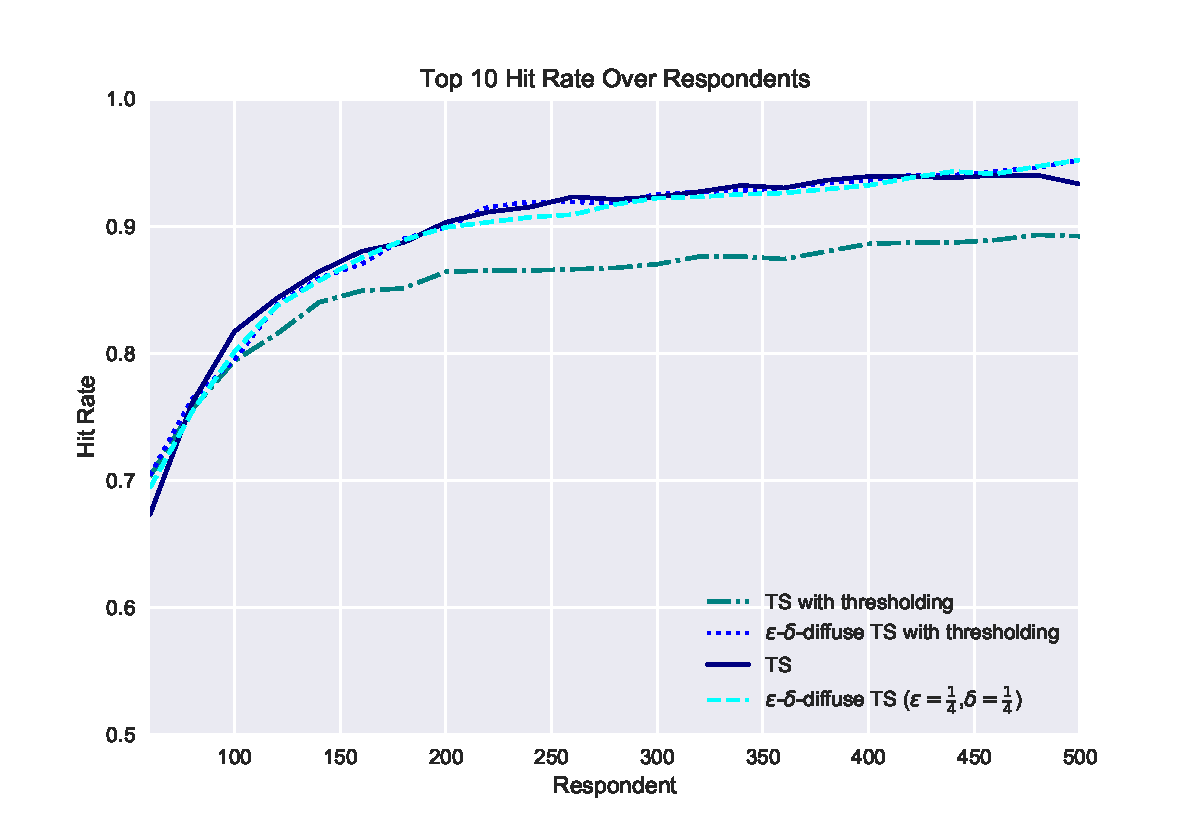
\includegraphics[width=.8\textwidth]{plots/hr120v20k10thres.pdf} }}%
    \qquad
    \subfloat[Top 20]{{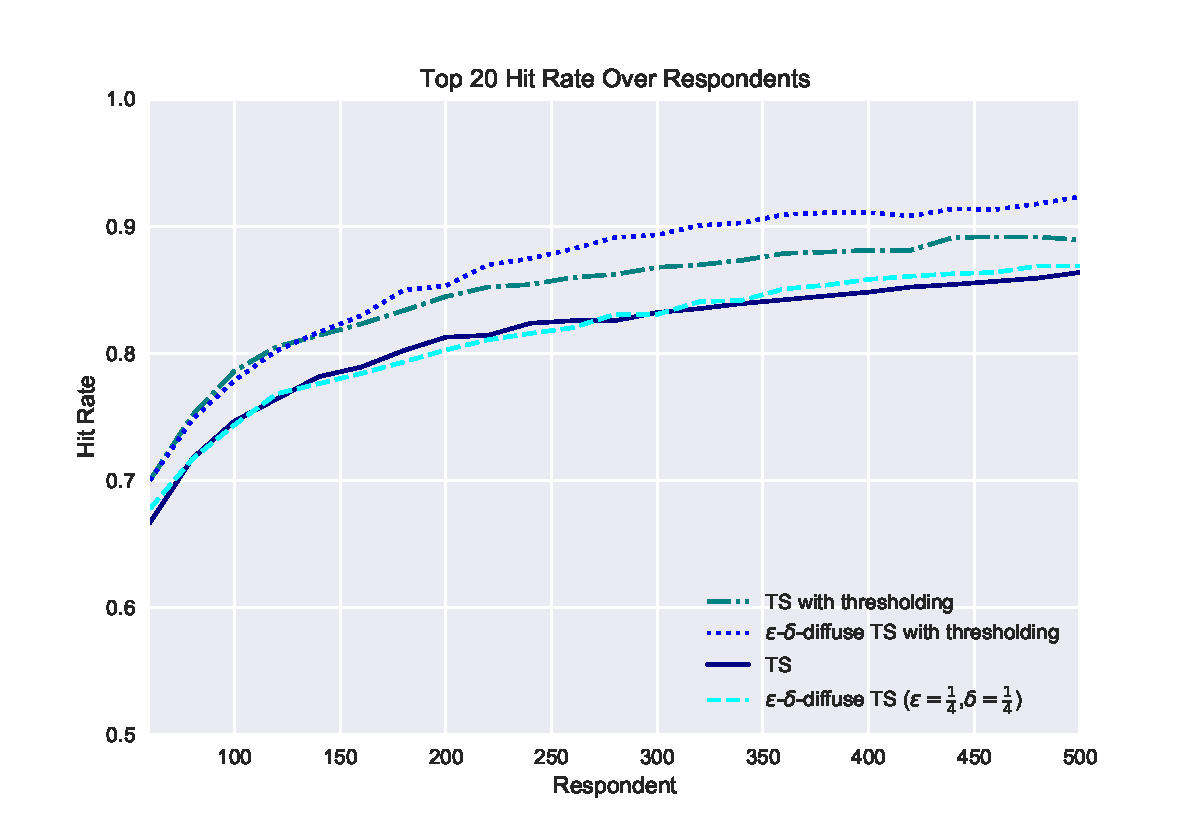
\includegraphics[width=.8\textwidth]{plots/hr120v20k20thres.pdf} }}%
	\end{center}
\end{figure}
%\eric{Why is \ts better than \tsthres for $k=10$?  Explain why in a good way \tsthres always does worse than \edtsthres. }


\begin{figure}%
    \caption{The plot shows hit rates for top $k=\{20,40\}$ with 120 items.}%
    \label{fig:K120_L20_k20hit_k40hit}%
 	\begin{center}
    \subfloat[Top 20]{{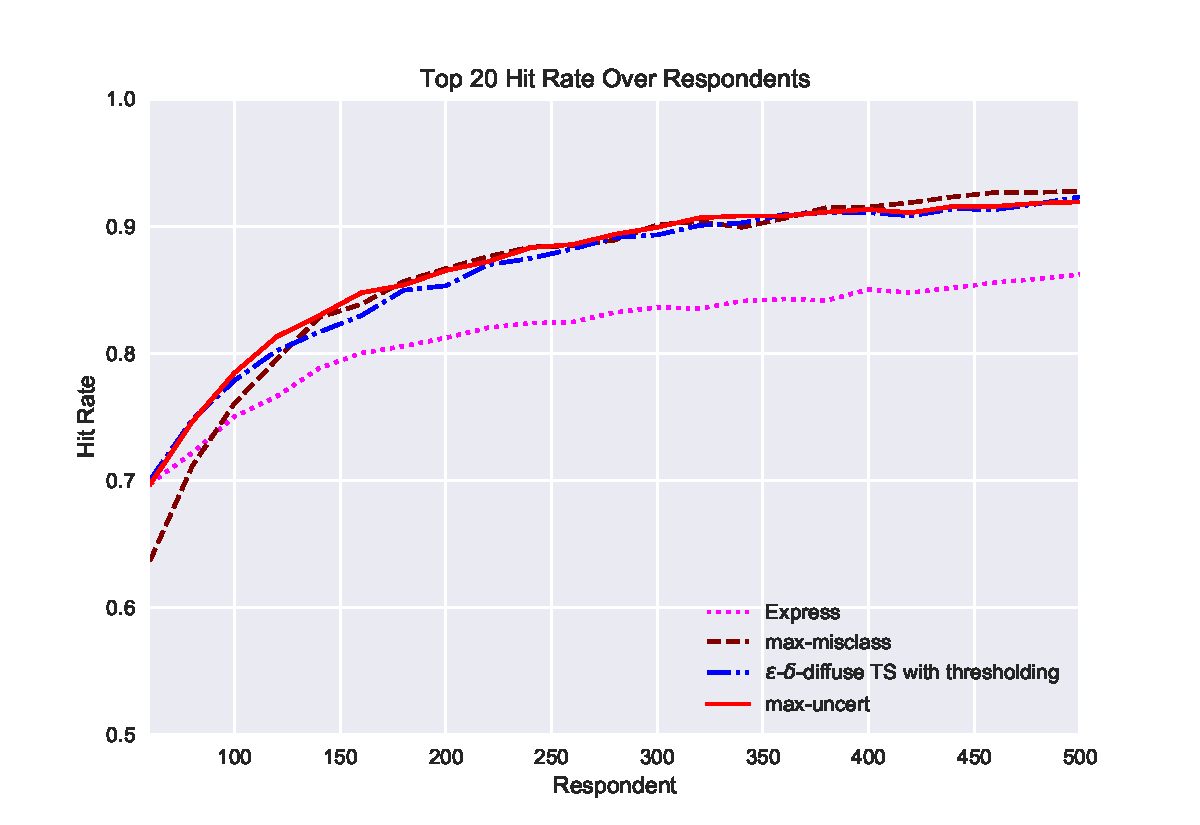
\includegraphics[width=.8\textwidth]{plots/hr120v20k20.pdf} }}%
    \qquad
    \subfloat[Top 40]{{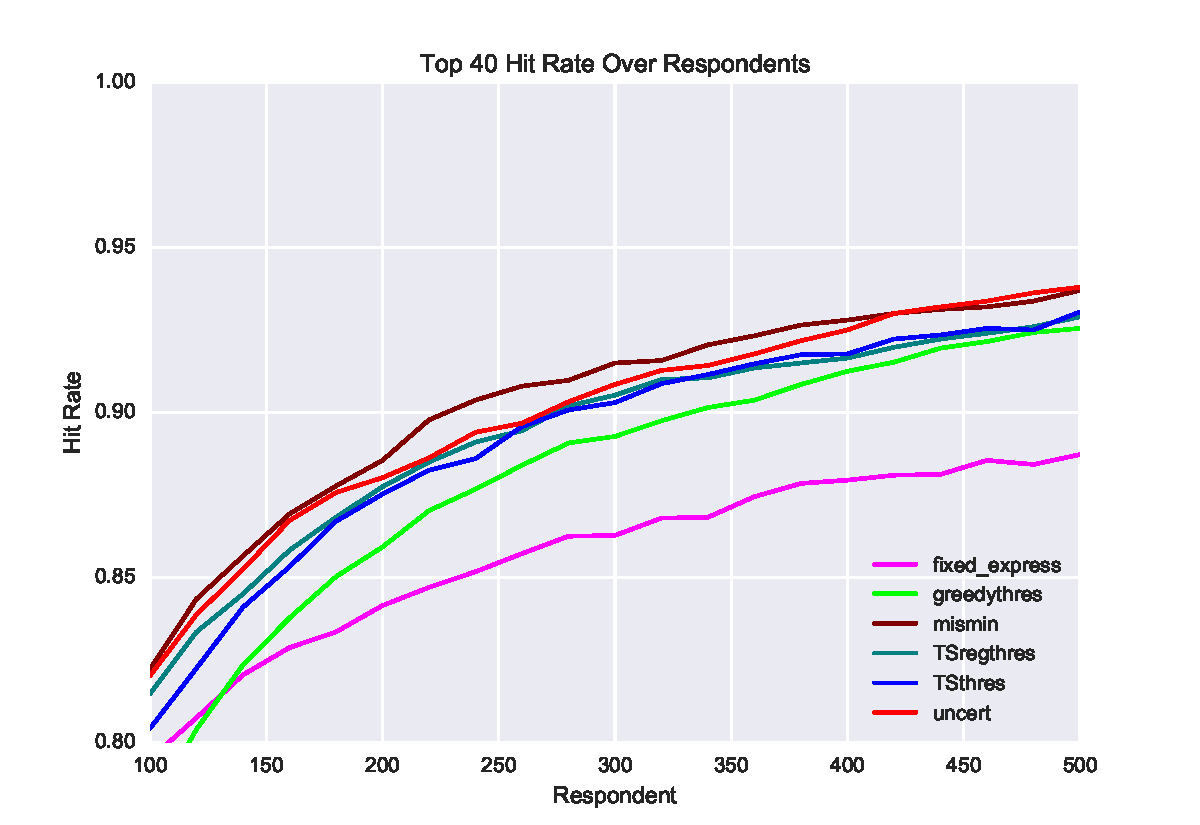
\includegraphics[width=.8\textwidth]{plots/hr120v20k40.pdf} }}%
    \end{center}
\end{figure}


% \begin{figure}
% \caption{3 Hit Rate with 120 items}
% 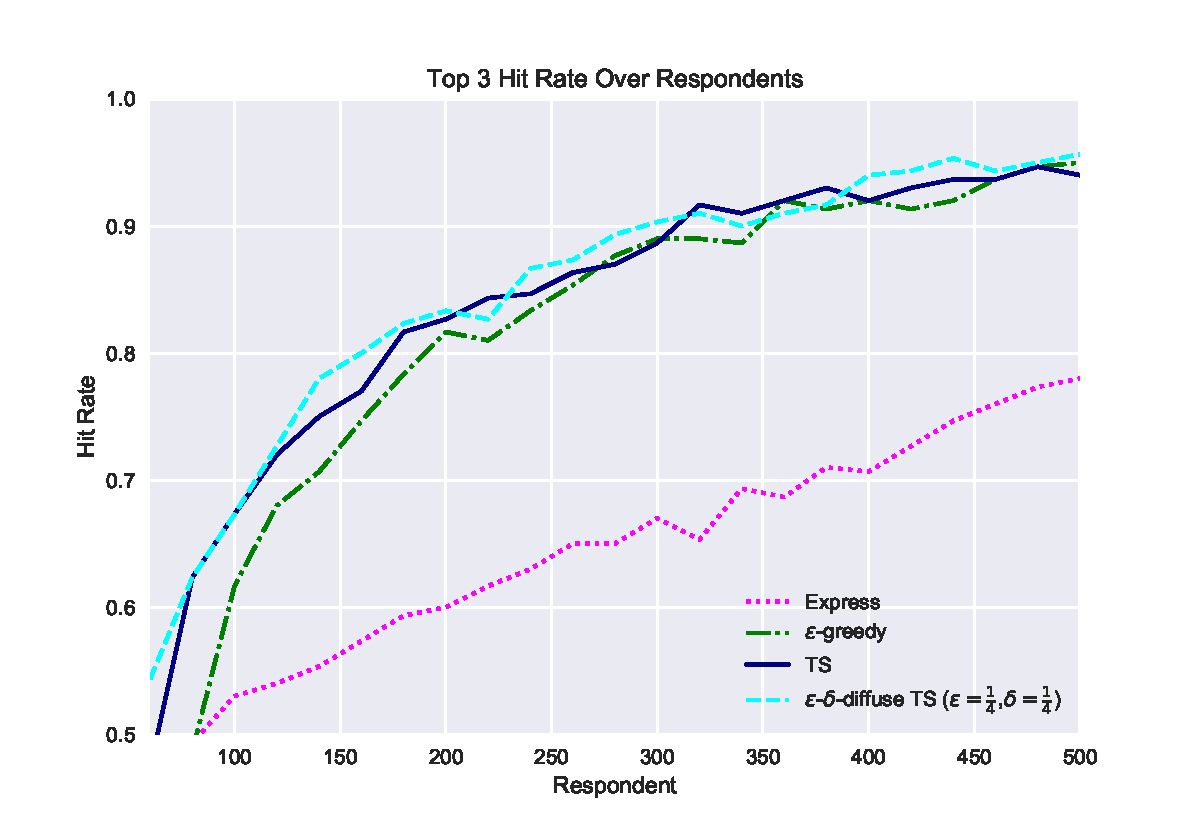
\includegraphics[width=1\textwidth]{plots/hr120v20k3.pdf}
% \label{fig:3hit}
% \end{figure}
% \begin{figure}
% \caption{10 Hit Rate with 120 items}
% 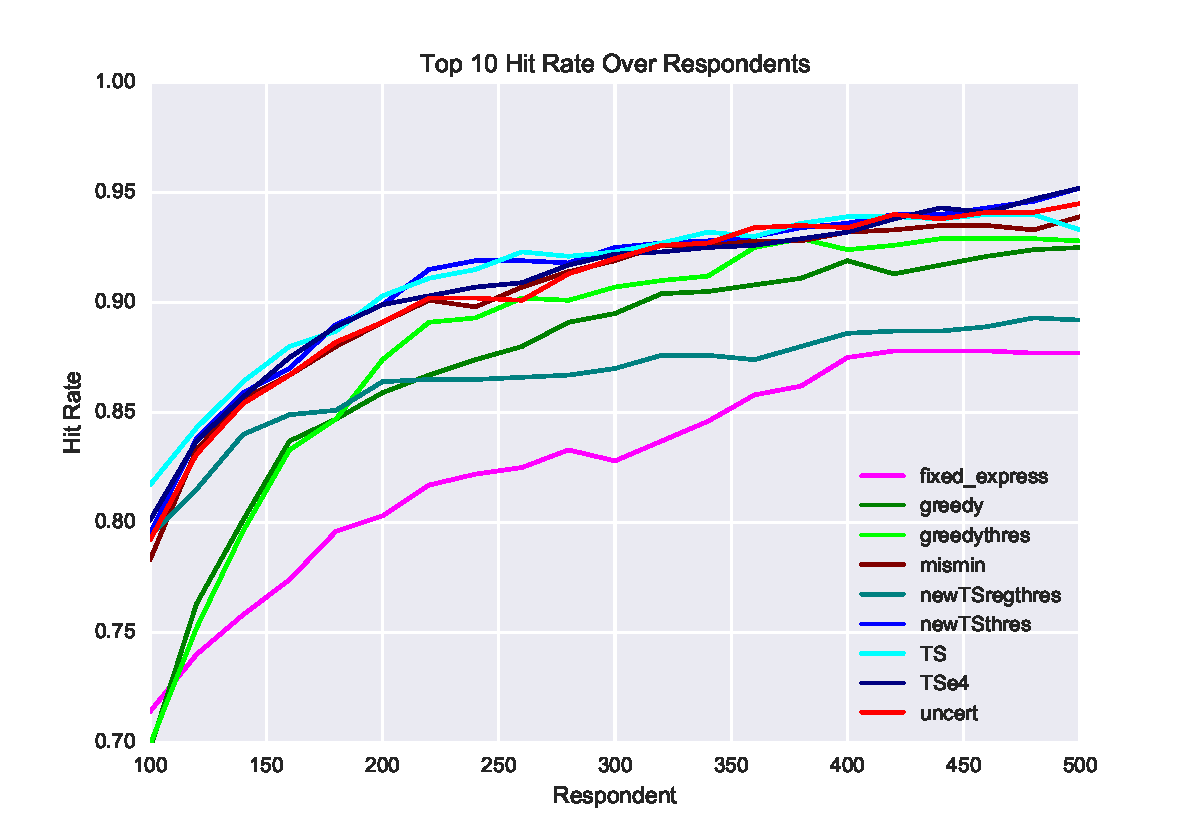
\includegraphics[width=1\textwidth]{plots/hr120v20k10.pdf}
% \label{fig:10hit}
% \end{figure}

% \begin{figure}
% \caption{20 Hit Rate with 120 items}
% 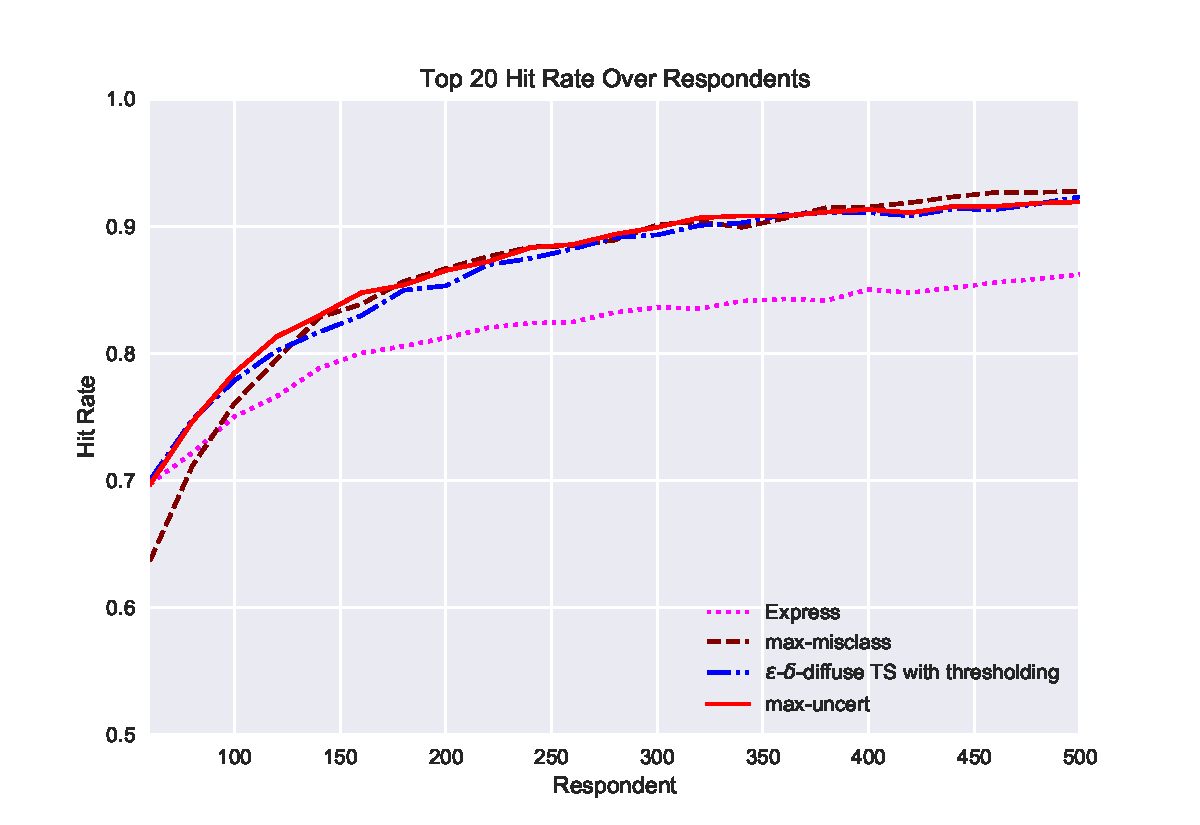
\includegraphics[width=1\textwidth]{plots/hr120v20k20.pdf}
% \label{fig:20hit}
% \end{figure}
% \begin{figure}
% \caption{40 Hit Rate with 120 items}
% 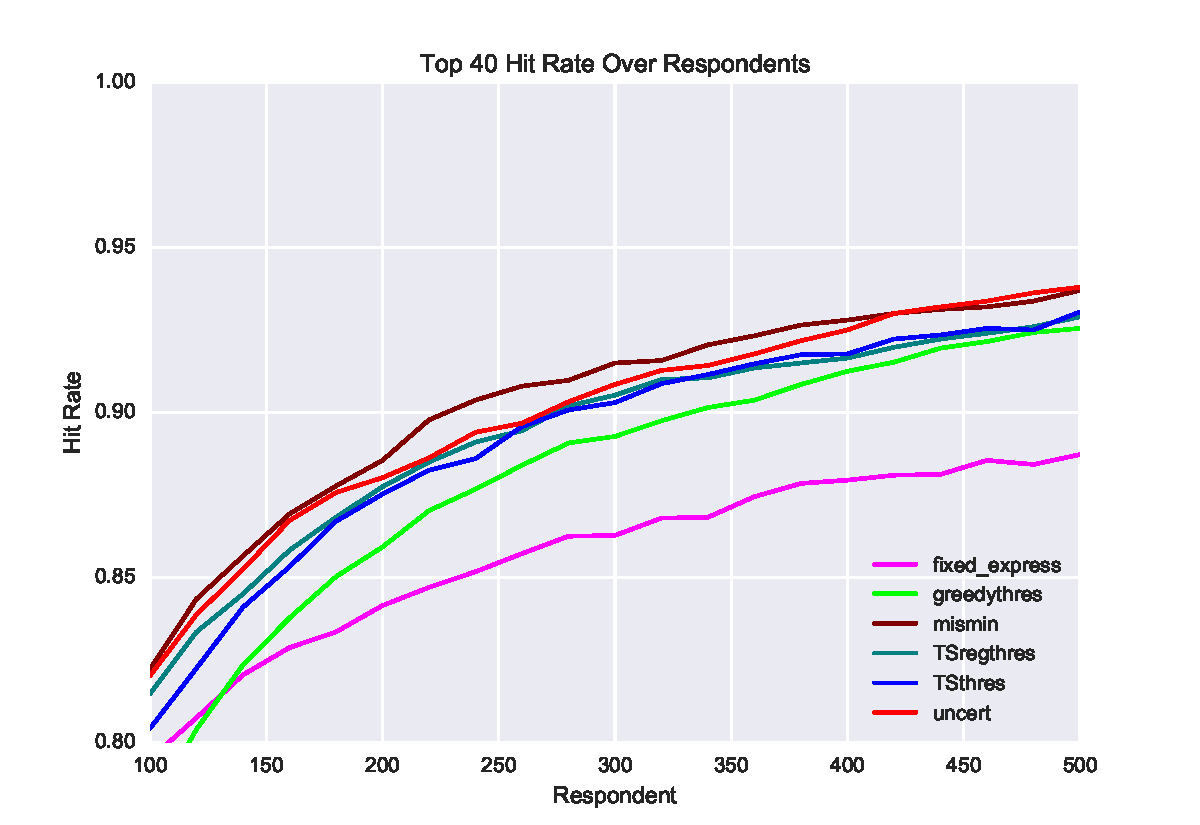
\includegraphics[width=1\textwidth]{plots/hr120v20k40.pdf}
% \label{fig:40hit}
% \end{figure}

\begin{table}
\caption{Top k Hit Rate at 260th and 500th Respondent with 120 Items}
\label{table:at_260_500}
\begin{center}
\begin{tabular}{llllllllll}
\hline 
\hline
\multicolumn{10}{l}{(a) After 260 respondents}\\
k &  \fixedexpressS&\egreedyS&\egreedythresS&\tsS&\edtsS&\tsthresS&\edtsthresS& \misminS& \uncertS \\ \hline
  3 & 0.65 &   0.85 &  0.86 &   0.86 & 0.87 & 0.78 & 0.86 &    0.88 &   0.84 \\
  10 &  0.83 &   0.88 & 0.90 &   0.92 & 0.91 & 0.87 & 0.92 &    0.91 &   0.90 \\
  20 & 0.82 & 0.78 &  0.86 & 0.83 & 0.82 & 0.86 & 0.88 &  0.88 &   0.89 \\  
  40 &  0.86 &   NA &  0.88 &  NA & NA & 0.89 & 0.90 &  0.91 &   0.90 \\
\hline
\hline
\end{tabular}
\begin{tabular}{llllllllll}
\multicolumn{10}{l}{(b) After 500 respondents}\\
k &  \fixedexpressS&\egreedyS&\egreedythresS&\tsS&\edtsS&\tsthresS&\edtsthresS& \misminS& \uncertS  \\
\hline
   3 & 0.78 &   0.95 & 0.93 & 0.94 & 0.96 & 0.83 & 0.97 &    0.95 &   0.94 \\
  10 &  0.88 &   0.93 &  0.93 &   0.93 & 0.95 & 0.89 & 0.95 &    0.94 &   0.95 \\  
  20 &  0.86 &   0.83 & 0.91 &  0.86 & 0.87 & 0.89 & 0.92 &  0.93 &   0.92 \\ 
  40 &  0.89 &   NA & 0.93 & NA & NA & 0.92 &  0.94 & 0.94 & 0.94 \\
\hline 
\hline
\end{tabular}
\end{center}
\end{table}



\begin{figure}%
    \caption{F}%
    \label{fig:winapprox_thresh_hit20}%
 	\begin{center}
    \subfloat[Top 20]{}%
    \qquad
    \subfloat[Top 20]{{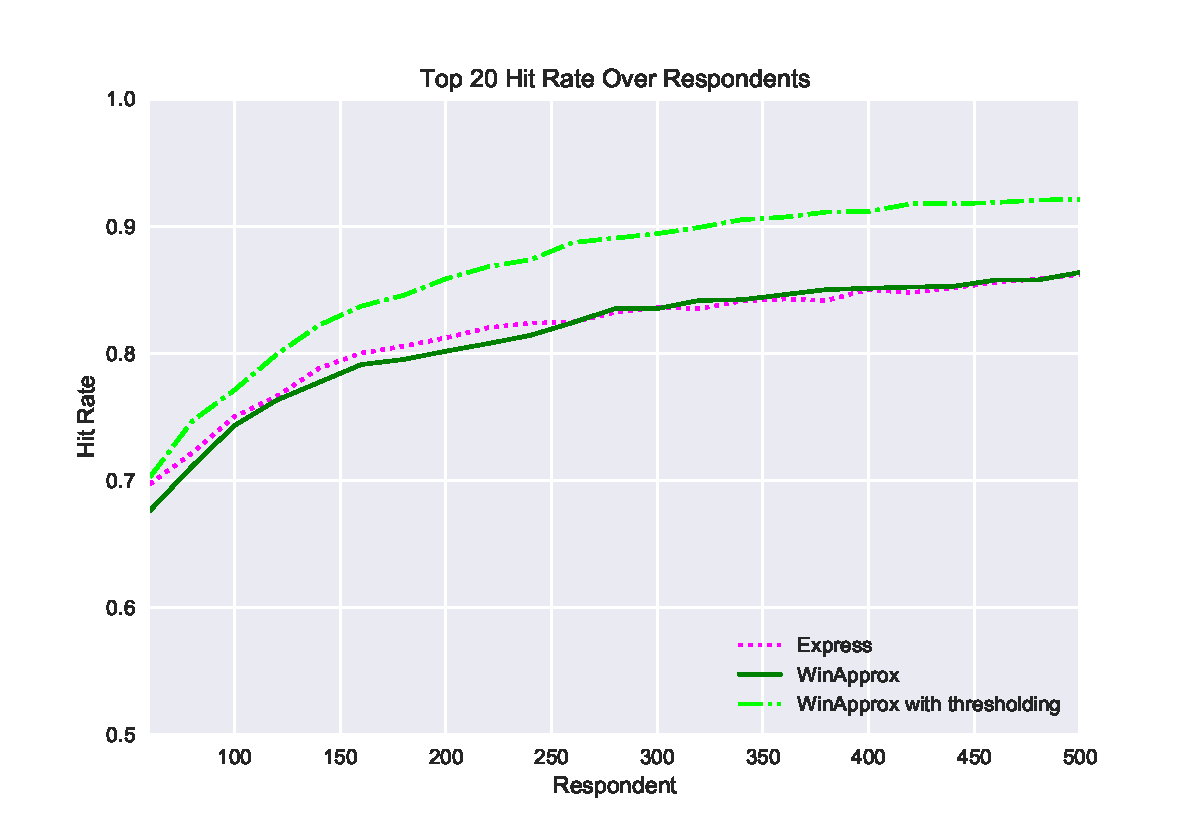
\includegraphics[width=.8\textwidth]{plots/hr120v20k20t2.pdf} }}%
	\end{center}
\end{figure}


% \begin{table}
% \caption{Top k Hit Rate for Various Algorithms at the 260th Respondent with 120 Items}
% \label{table:at260}
% \begin{center}
% \begin{tabular}{llllllllll}
% \hline   k &  fixed\_express &  greedy &  greedythres &  mismin &    TS &  TSe4 &  TSregthres &  TSthres &  uncert \\ \hline  3 &          0.650 &   0.853 &        0.860 &   0.883 & 0.863 & 0.873 &       0.850 &    0.893 &   0.840 \\  10 &          0.825 &   0.880 &        0.902 &   0.907 & 0.923 & 0.909 &       0.909 &    0.907 &   0.901 \\  20 &          0.824 &   0.784 &        0.863 &   0.885 & 0.825 & 0.820 &       0.869 &    0.879 &   0.886 \\  40 &          0.857 &   NA &        0.884 &   0.908 & NA & NA &       0.895 &    0.888 &   0.897\end{tabular}
% \end{center}
% \end{table}

% \begin{table}
% \caption{Top k Hit Rate for Various Algorithms at the 500th Respondent with 120 Items}
% \label{table:at500}
% \begin{center}
% \begin{tabular}{llllllllll}
% \hline   k &  fixed\_express &  greedy &  greedythres &  mismin &    TS &  TSe4 &  TSregthres &  TSthres &  uncert \\ \hline   3 &          0.780 &   0.950 &        0.933 &   0.950 & 0.940 & 0.957 &       0.917 &    0.947 &   0.943 \\  10 &          0.877 &   0.925 &        0.928 &   0.939 & 0.933 & 0.952 &       0.940 &    0.947 &   0.945 \\  20 &          0.862 &   0.827 &        0.914 &   0.928 & 0.863 & 0.868 &       0.916 &    0.914 &   0.919 \\  40 &          0.887 &   NA &        0.926 &   0.937 & NA & NA &       0.929 &    0.927 &   0.938 \end{tabular}
% \end{center}
% \end{table}



\begin{figure}%
    \caption{F}%
    \label{fig:winapprox_thresh_hit20}%
 	\begin{center}
    \subfloat[Top 20]{}%
    \qquad
    \subfloat[Top 20]{{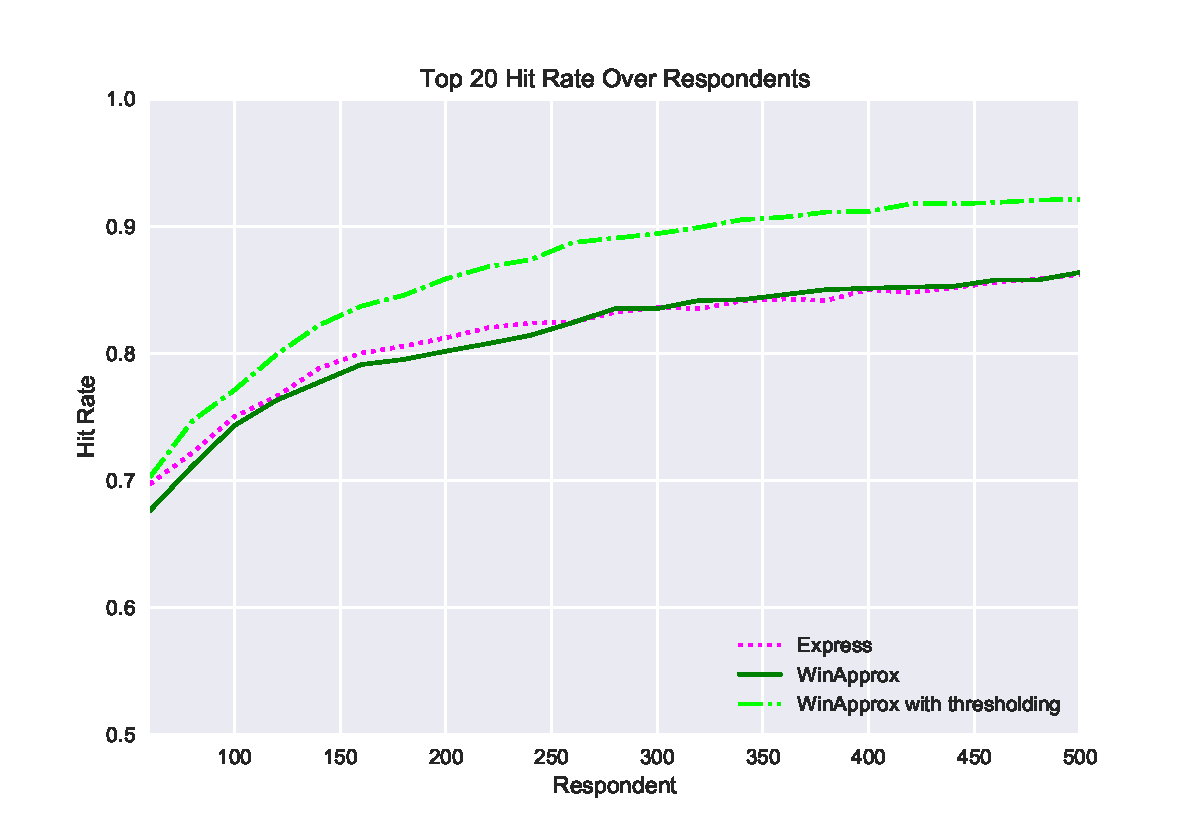
\includegraphics[width=.8\textwidth]{plots/hr120v20k20t2.pdf} }}%
	\end{center}
\end{figure}


Our results show algorithm performance depends on the hit rate measure relative to the number of items selected ($k$ versus $\numperset$). For $k \ge L$, the best performers are Greatest Uncertainty with random perturbations (\uncert) and Misclassification Minimization with random perturbations (\mismin). The methods perform nearly as well as the best algorithms for $k < L$, $\epsilon$-diffuse Thompson Sampling with thresholding (\edtsthres) and without thresholding (\edts).



% \eric{Add a Takeaway from each section beginning here.} In conclusion, \textbf{we find ... }

\section{Robustness tests} \label{sec:robust}


\subsection{Non-Stationary Distribution: Misinformed Starts}

%\alexander{Look at hr120v20k3moremis1top10.pdf, hr120v20k3moremis2top10.pdf, hr120v20k3moremis2top5.pdf, hr120v20k3moremis1top5.pdf, and see if you want to add in those results (for the 1st 150 respondents percentile of top 3 items is (resp number)/2)}

As a survey is conducted, the sample of early respondents may not be uniformly representative from the preferences of the rest of the true underlying population. We want to ensure that the proposed methods are robust to some extent of mis-representativeness early, but without specifying the particular mechanism of the sample selection. We refer to this settings as a \emph{misinformed start}. Specifically, we illustrate it by examining this: What would happen if the first 50 respondents to a survey are not representative of the sample's average preferences? We use this because it reflects an extreme version of a real pattern. Depending on how rapidly a marketing researcher may invite a panel to respond to a survey, the first set of respondents may share some atypical characteristics (e.g., over-eager, anxious, available to take the survey at a particular time).

For the simulations reported in table \ref{table:120mis}, the first 50 simulated respondents mimic respondents randomly drawn utilities as before, but they are manipulated to behave as if the truly most three preferred items are actually have the utilities of some of the least preferred items. In particular, we set the utilities for the population's top three true items to be equal to the bottom 25th percentile, and we do this separately for each respondent's true utilities in the data-generating process. After the misinformed start, the remaining respondents are well-behaved, drawn using bootstrap sampling, with true individual-level preferences as given in the original P\&G dataset and used in our main analysis.

\begin{table}
\caption{Misinformed Start: Top 3 Hit Rate}
\begin{tabular}{llllllllll}
\hline   Resp &  \fixedexpressS&\egreedyS&\egreedythresS&\tsS&\edtsS&\tsthresS&\edtsthresS& \misminS& \uncertS   \\ \hline    260 &   0.09 &   0.30 & 0.24 & 0.07  & 0.35 & 0.07 &  0.36 & 0.25 &   0.27 \\
  500 &  0.25 &   0.57 &  0.49 &  0.13 & 0.54 &   0.10 &    0.64 & 0.54 &  0.50  \end{tabular}
\begin{center}
\caption{Top 3 hit rate is shown as of the 260th and 500th respondent with $\numitems=120$ items.} \label{table:120mis} 
\end{center}
\end{table}

The misinformed start simulation presents a particularly perverse situation, one that could be considered worse than anything marketers might see in practice. So strong performance in situation suggests robustness to non-stationarity in preference or respondent self-selection during the sampling window. We illustrate that robustness in Table \ref{table:120mis}. The standard \ts perform worse than the Fixed Express MaxDiff algorithm with misinformed starts. However, the added randomness in the Bandit MaxDiff \edts approach is critical as that mixture of a diffuse and regular posterior allows it to continue investigating the value of incorrectly estimated low preference items among later respondents. While \mismin and \uncert also are fairly robust, the \edts version of Bandit MaxDiff, performs even better achieving a higher hit rate earlier on (0.35 vs. 0.27 as of 260th respondent after 0.00 after the 50th). Further, the \edts is less-computationally intensive than those algorithms inspired by active-learning.

The robustness to a dramatic non-stationarity meant to throw all algorithms off is a strong feature of our proposed approach, specifically the scalable \edts for MaxDiff. 

\subsection{Varying Number of Items}


We also considered the case of 300 items, and we find that the benefits of the proposed algorithms are only further increased.


\subsubsection{Increasing Items}
\begin{table}
\caption{Top k Hit Rate at 260th Respondent with 300 Items}
\begin{center}
\begin{tabular}{lllllllllll}
\hline   k &  \fixedexpressS & \egreedyS&\egreedythresS&\tsS&\edtsS&\tsthresS&\edtsthresS& \misminS& \uncertS \\ \hline 
3&   0.31 &   0.59 & 0.48 & 0.60 &  0.64 & 0.54 & 0.65 & 0.54 &   0.58 \\ 
10 & 0.46 &   0.61 & 0.54 & 0.63  & 0.66 & 0.58 & 0.68 & 0.68  &   0.69 \\ 
20 & 0.55 &   0.60 & 0.59 &  0.61 & 0.66 & 0.59 & 0.71 &       0.72 &   0.72\\ 
40 & 0.62 &   NA & 0.62 & NA &  NA & 0.64 & 0.70 & 0.71 & 0.72 \end{tabular}
\end{center}
\label{table:300at260}
\end{table}

\begin{table}
\caption{Top k Hit Rate at 500th Respondent with 300 Items}
\begin{center}
\begin{tabular}{lllllllllll}
\hline   k &  \fixedexpressS & \egreedyS&\egreedythresS&\tsS&\edtsS&\tsthresS&\edtsthresS& \misminS& \uncertS  \\ \hline  
3 & 0.39 &  0.76 & 0.75 & 0.72 & 0.79 & 0.61 &  0.80 &  0.77 &0.78 \\
10 &  0.58 &   0.76 & 0.72 & 0.70 & 0.78 & 0.63 & 0.79 & 0.79 &   0.79\\
20 & 0.68 & 0.72 & 0.76 & 0.67 & 0.76 &  0.63 & 0.82 & 0.84 &    0.85 \\ 
40 & 0.72 &   NA & 0.75 & NA & NA & 0.69 & 0.80 &0.81 & 0.83 \end{tabular}
\end{center}
\label{table:300at500}
\end{table}
Would the benefits of adaptive MaxDiff algorithms observed with 120 items hold for 300 items? While no dataset of utilities from human respondents on 300 possible product features or benefits is available, we generate a data by leveraging the 120-item set provided by P\&G. To generate preferences across an additional 180 items, we combine pairs of existing items according to a randomly distributed weighting scheme, with additional random variation added. The result is a 300-item MaxDiff dataset based on the original preferences of 981 respondents.

The advantages seen in the 120-item results are improved using 300 items. Tables \ref{table:300at260} and \ref{table:300at500} show the well-informed start results. The adaptive approaches show substantial gains over the Fixed Express MaxDiff approach on the top-3, -10, -20, and -40 hit rate criterion.

\subsubsection{Decreasing Items}

\begin{table}
\caption{Top k Hit Rate 40 Items}
\begin{center}
\begin{tabular}{lllllllllll}
\hline   Resp & k &  \fixedexpressS & \egreedyS&\egreedythresS&\tsS&\edtsS&\tsthresS&\edtsthresS& \misminS& \uncertS  \\
\hline 
260 & 3 & 0.90 & 0.97 &  0.97 &  0.97 & 0.97 & 0.97 &  0.96 & 0.94 &  0.94 \\  10 & 0.87 & 0.90 & 0.91 &  0.93 & 0.91 & 0.91 & 0.91 & 0.91 &  0.92  \\ 
500 & 3 & 0.93 & 0.99 & 0.99 & 0.99 & 0.99 & 0.98 & 0.98 & 0.98 &  0.99 \\  10 & 0.90 &   0.92 &  0.93  & 0.94 & 0.94 & 0.93 &    0.92 & 0.93 &  0.93 \end{tabular}
\end{center}
\label{table:40at260and500}
\end{table}

How do the adaptive models perform using a more traditional MaxDiff set of 40 items? Using a random 40-item subset from the original set of 120 items, the Express MaxDiff design shows each item to every other respondent on average, more than in larger item cases. While this problem is easier than others, as exhibited by the high hit rates, still, the adaptive MaxDiff approaches perform better than traditional MaxDiff models (Table \ref{table:40at260and500}).

%By reducing the number of items to 40 and changing the number of tasks to 12, the fixed express design can now show each item an average of 1.5 times per respondent, which is much less sparse than in larger item cases.\\


\subsection{Additional datasets: real and synthetic}

We now show the performance of the same set of algorithms on two entirely different datasets. First, we use data from a study of claims for cleaning products administered by Skimm Group. We derive a simulation environment just as we did in the main analysis section with the P\&G study run by Sawtooth Software. The simulation setting is largely same, except the Cleaning Product Study has $\numitems=86$ items, and we update every batch of 10 rather than 20 respondents. Table \ref{table:skim} shows that the task of identifying the top sets of items here was quite a bit easier than in the P\&G study, and still the proposed methods perform better than the non-adaptive and slightly better than naive adaptive approaches. It also offers a confirmation that under such settings where the best items are obvious, the proposed methods' performance at worst collapses to a less sophisticated method's performance. 

To further show another illustration, we create a purely synthetic dataset. As a baseline for such a dataset, we sample population-level mean item utilities $u_i(\theta)$ from a uniform distribution for $i=1,\ldots,100$. Each respondent's preference utility is sampled from a normal distribution with mean $u_i(\theta)$ and variance 1, i.e., adding standard normal noise. The variance of that noise is mild enough so that the rankings of items for each respondent are highly correlated. As before, we take the top $k$ highest  mean preference scores across the respondents, $u_i(\theta)$,  to be the top $k$ true items, and proceed with the simulation using the same structure, but $\numitems=100$. The results shown in Tables \ref{table:sim} reflect the consistent performance again.



\begin{table}
\caption{Top k Hit Rate at 250th and 500th Respondent with 86 Items from Cleaning Product Study from Skimm Group}
\label{table:skim}
\begin{center}
\begin{tabular}{llllllllll}
\hline 
\hline
\multicolumn{10}{l}{(a) After 250 respondents}\\
k &  \fixedexpressS&\egreedyS&\egreedythresS&\tsS&\edtsS&\tsthresS&\edtsthresS& \misminS& \uncertS \\ \hline
%  3 & 0.90 &   1.00 &  NA &   0.97 & 0.99 & NA & NA &    0.98 &   0.97 \\
  10 &  0.88 &   0.90 & 0.92 &   0.91 & 0.92 & 0.89 & 0.91 &    0.93 &   0.92 \\
  20 & 0.91 & 0.87 &  0.96 & 0.86 & 0.91 & 0.92 & 0.96 &  0.96 &   0.92 \\  
%  40 &  0.92 &   NA &  0.95 &  NA & NA & 0.94 & 0.95 &  0.96 &   0.95 \\
\hline
\hline
\end{tabular}
\begin{tabular}{llllllllll}
\multicolumn{10}{l}{(b) After 500 respondents}\\
k &  \fixedexpressS&\egreedyS&\egreedythresS&\tsS&\edtsS&\tsthresS&\edtsthresS& \misminS& \uncertS  \\
\hline
%   3 & 0.94 & 1.00 & NA & 0.98 & 1.00 & NA & NA & 1.00 &   0.99 \\
  10 &  0.91 &   0.92 &  0.93 &   0.92 & 0.93 & 0.90 & 0.93 &    0.93 &   0.94 \\  
  20 &  0.94 &   0.90 & 0.98 &  0.89 & 0.94 & 0.94 & 0.98 &  0.98 &   0.98 \\ 
%  40 &  0.95 &   NA & 0.97 & NA & NA & 0.96 &  0.97 & 0.97 & 0.97 \\
\hline 
\hline
\end{tabular}
\end{center}
\end{table}


\begin{table}
\caption{Top k Hit Rate at 260th and 500th Respondent with Simulated Data Set}\label{table:sim}
\begin{center}
\begin{tabular}{lllllllllll}
\hline  Resp &  k &  \fixedexpressS & \egreedyS&\egreedythresS&\tsS&\edtsS&\tsthresS&\edtsthresS& \misminS& \uncertS \\ \hline
260 &  10 & 0.77 &   0.88 & 0.88  & 0.87&0.89 & 	0.88&0.89 & 0.89 &  0.88 \\  20 &  0.87 &  0.86 &   0.92  & 0.88&0.90 &  	0.93&0.94&  0.93 &  0.93 \\  
500 & 10 & 0.85&0.92&0.92 & 0.93&0.94 & 0.92&0.94&0.93 &   0.93 \\  20 & 0.90&0.90&0.95& 0.90 &0.93 & 0.95&0.96 &0.96& 0.96 \\
\hline
\end{tabular}
\end{center}
\end{table}



\section{Extensions considering utility values beyond rank}


\subsection{True Utility as Hit-Rate Generalization}

We have used hit rate as an indicator of performance in the classification task of selecting the top set of items. But we recognize that this a dichotomization of a continuous measure. Instead of just looking at the estimated relative rank of the top set of items and the rest, we consider the implication of that in terms of actual item utility. For instance, to differentiate between an algorithm that puts the top nine items and the 11th item in the top 10 and one that puts the top nine items and the 40th item in the top 10, we would want to consider the actual values of those items. Therefore, we define \emph{percent true utility} ($PTU$). First, the exponential weighted sum of true utilities of the items in a set. So we consider, $\mu_\pi=\sum_{\pi(i) \in \topset(\pi)} e^{u_\pi(i)(\theta)}$, where $\topset(\pi)$ denote the current estimate of the top $k$ items based on a predicted ranking $\pi$. And we let $\mu^{*}$ be the corresponding sum for the items in the $\topset^{*}(\theta)$, the true top set of $k$ items. Then, the $PTU = \frac{\mu_\pi}{\mu^{*}},$ the estimated exponential weighted sum of true utilities of the selected top $k$ items based on respondents so far divided by the maximum value of the exponential weighted sum of true utilities that could be attained with $k$ items of the total of $\numitems$. 

In this sense, PTU is a generalization of simple hit rate, and it can be used to further differentiate the algorithms. We measure performance of algorithms on the main empirical setting, $\numitems=120,\numperset=20,J=12,|S|=5$, and measuring top $k=20$. While the hit rate shows the Fixed Express, \ts, and \edts algorithms to perform similarly, PTU illustrates how \edts has an edge over \ts and Fixed Express (Figure \ref{fig:20util}).  This becomes a problem of learning the rank ordering of the values of $\mu^s$ for all sets $s$, and a variety of such subsets are shown in Table \ref{table:PTU} in terms of their PTU.

\begin{figure}
\caption{Performance in terms of percentage of true utility for the top 20 of 120 items.}
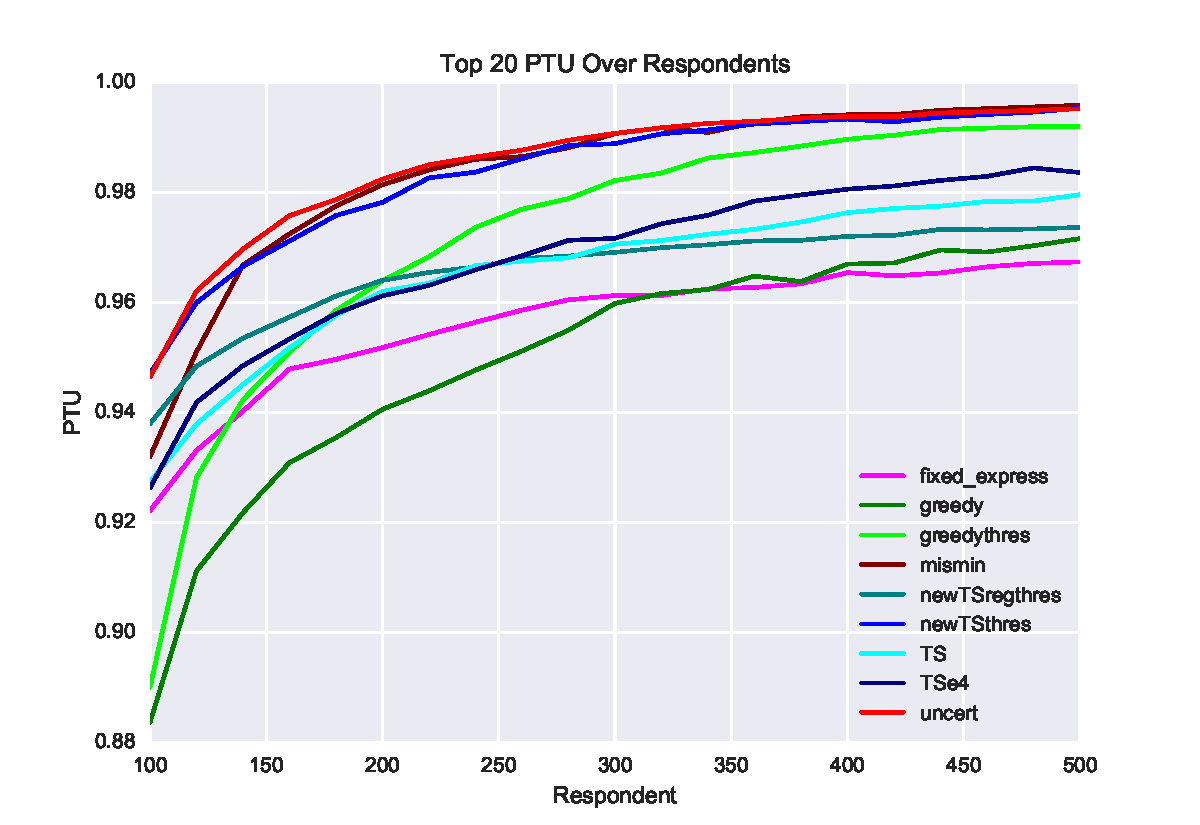
\includegraphics[width=1\textwidth]{plots/PTU120v20k20.pdf}
\label{fig:20util}
\end{figure}
\begin{table}
\caption{PTU for Various $S$ for P\&G Data Top 3}
\begin{center}
\begin{tabular}{c | c }
$S$& Percent True Utility \\
\hline
\{1,2,3\}& 1.0 \\
\{1,2,4\}&.973 \\
\{1,2,5\}&.948 \\
\{1,3,4\}&.934 \\
\{1,3,5\}&.910 \\
\{1,4,5\}&.882 \\
\{2,3,4\}&.922 \\
\{2,3,5\}&.897 \\
\{2,4,5\}&.870 \\
\{3,4,5\}&.831 \\
\hline
\end{tabular}
\end{center}
\label{table:PTU}
\end{table}

\subsection{Stopping Rules: Posterior Distribution Regret and Value Remaining}

Almost all our results show diminishing algorithm performance at some point as we administer more surveys. Therefore, it becomes inefficient to continue surveying after a certain number of respondents. In practice, we do not know this point a priori. So how do we know when to stop?

Adapted from~\cite{scott2015multi} and~\cite{scott2010modern} for multi-armed bandit problem solving, the value remaining in the experiment is the posterior distribution of $\frac{\mu_{S^*}-\mu_{S}}{\mu_{S}}$, where $\mu_{S^*}$ is the largest value of the exponential weighted utility and $\mu_{S}$ is the exponential weighted utility of the set most likely to be optimal, denoted $S$. We take $n$ Bayes Bootstrap draws from the posterior, letting $\mu_{S^*}^{m}$ be the maximum exponential weighted utility of draw $m$ and $\mu_{S}^{m}$ be the utility using draw $m$ from set $S$. We let $\Delta^{m}=\frac{\mu^m_{S^*}-\mu^m_{S}}{\mu^m_{S}}$.

\begin{table}
\begin{center}
\caption{Draws of Items' Exponential Utility after 100 Iterations}
\label{table:data}
\begin{tabular}{l | c c c c c c c c}
& \multicolumn{8}{c}{Current belief: rank order of items by utility} \\
& 1st &  2nd  &  3rd  &  4th &  5th & 6th & 7th &  8th \\
\hline
% \multicolumn{9}{l}{Posterior draws of utility} \\
Draw 1 & 4.02 &  3.50 &  5.08 & 4.16&  4.22 & 4.41 & 3.65 &  3.27 \\
Draw 2 &4.18 & 4.72 & 3.49 & 3.48 & 3.63 & 3.60 & 3.56 &  3.70 \\
Draw 3 &4.81 & 5.23 & 5.04 &  3.96 &  4.17 & 4.37 &  3.58 & 2.99 \\ 
\end{tabular}
\end{center}
\end{table}

\begin{figure}
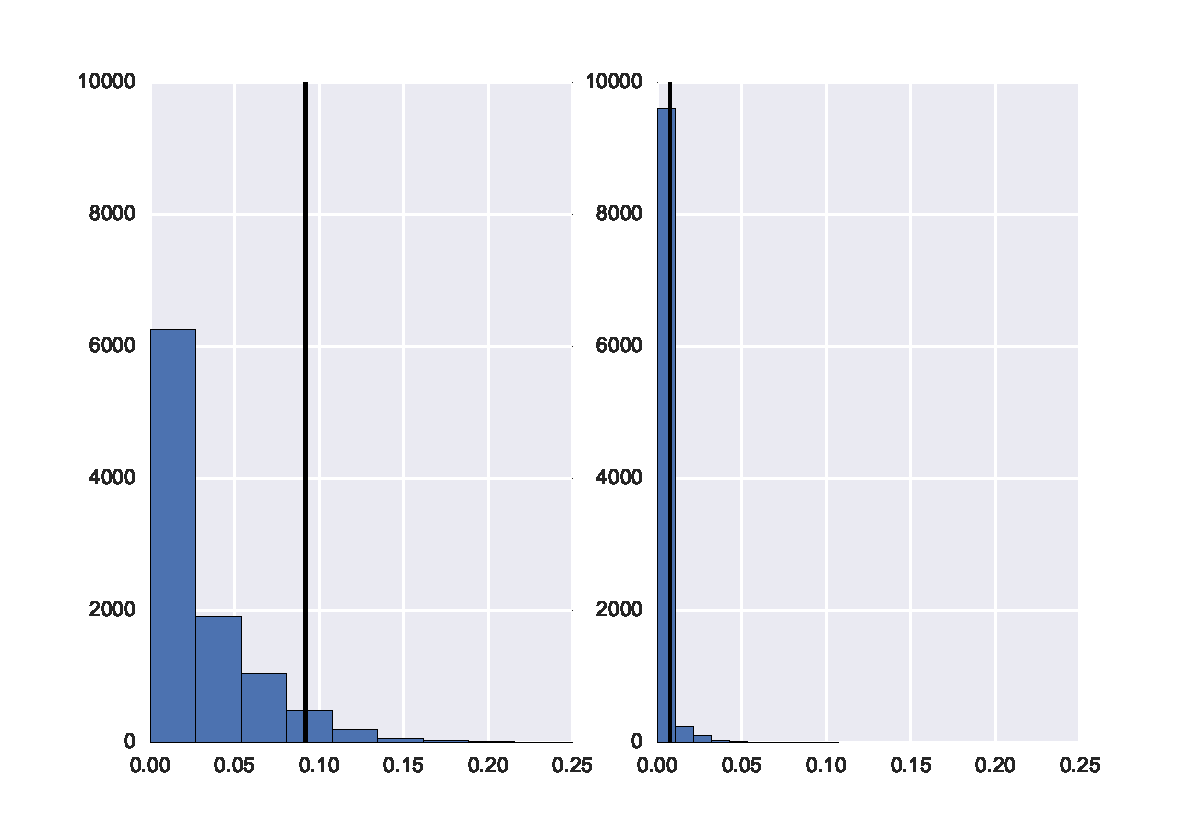
\includegraphics[width=1\linewidth]{plots/valremhist.pdf}
\caption{Two histograms of $\Delta$ are shown. At left, after 100 iterations, the potential value remaining is 0.092. At right, after 220 iterations, the potential value remaining is 0.008.}
\label{fig:data}
\end{figure}

Table \ref{table:data} shows the exponential weighted utility of a single item. The columns are in current rank order and show the top eight utilities. $S$ is the set containing the current first, second, and third ranked items. Then, $\mu^1_{S}=4.02+3.50+5.08=12.6$ and $\mu_{S^*}^{1}=5.08+4.41+4.16=13.65$, so $\Delta^{1}=\frac{13.65-12.6}{12.6}=.083$. Likewise, $\Delta^{2}=\frac{12.6-12.39}{12.39}=.017$ and $\Delta^{3}=\frac{15.08-15.08}{15.08}=0$. (Note $\Delta^m=0$ when $S$ contains the top utilities.) The histogram of $\Delta$ after 100 iterations and 220 iterations is shown in figure \ref{fig:data}.

The potential value remaining (PVR) is the 95 quantile of the distribution $\Delta$ (Figure \ref{fig:data}). After 100 iterations, PVR is 0.092. While we do not know the utility of $S$, we know an alternative set might perform better by as much as 9.2\%.

\text{plots/3vr120show3.pdf}
\text{plots/3vr120show3ex.pdf}

 %\alexander{Replace this plot with stophisted02.pdf stophistprob02.pdf and stophistTSgr02.pdf}

\begin{figure}
\caption{Average stopping times are shown with various thresholds.}
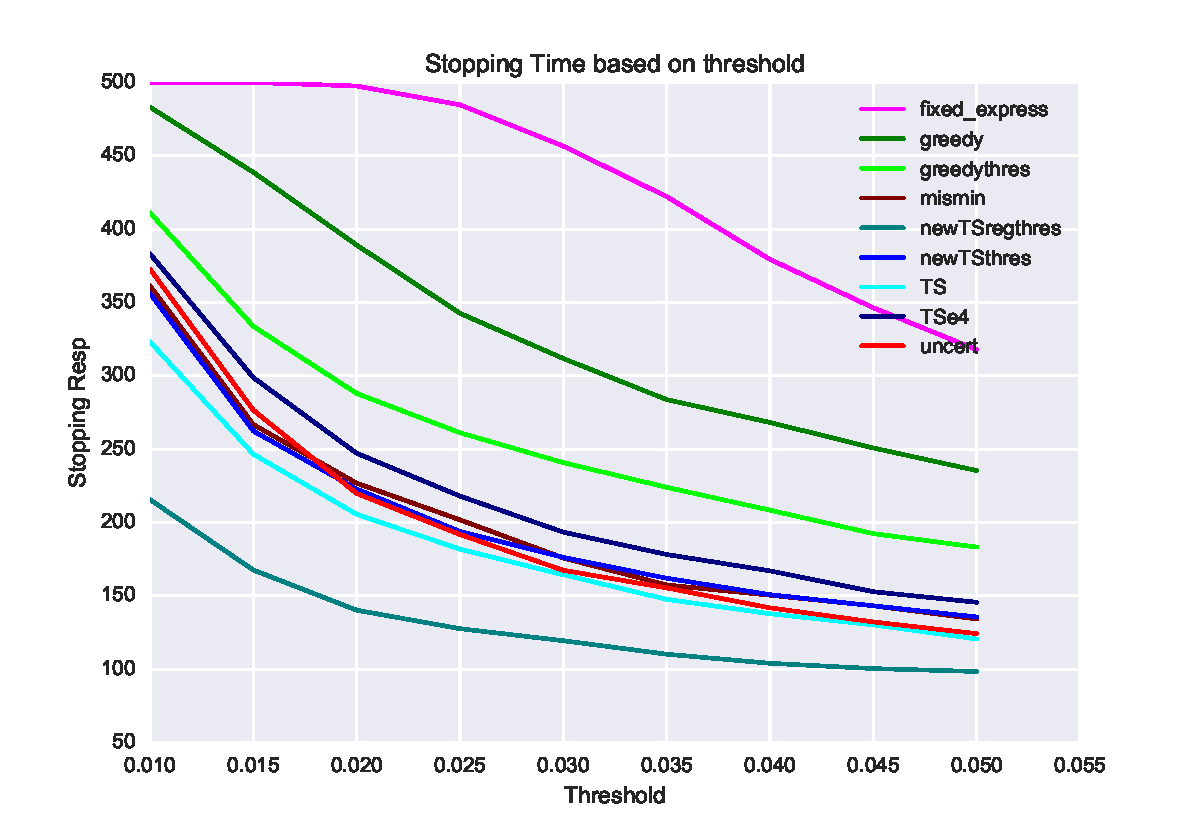
\includegraphics[width=1\textwidth]{plots/stoppingtimes.pdf}
\label{fig:st}
\end{figure}
\begin{table}
\begin{center}
\caption{Average Stopping Time and Hit Rate With PVR Threshold 0.05 for Top 10 Items}
\label{table:st5}
\begin{tabular}{llllllllll}
\hline    &  fixed\_express &  greedy &  greedythres &  mismin &    TS &  TSe4 &  TSregthres &  TSthres &  uncert \\\hline  Avg ST  & 318 &   235 & 183 & 134 & 121 & 146 & 	98 &	136 &   124 \\  Avg hr  &  0.854 &  0.88 & 0.852&0.848 & 0.846 & 	0.866 & 0.795 &0.857 &  0.837 \end{tabular}
\end{center}
\caption{Average Stopping Time and Hit Rate With PVR Threshold 0.02 for Top 10 Items}
\label{table:st2}
\end{table}
\begin{table}
\begin{center}
\begin{tabular}{llllllllll}
\hline    &  fixed\_express &  greedy &  greedythres &  mismin &    TS &  TSe4 &  TSregthres &  TSthres &  uncert \\\hline    Avg ST & 498 & 389 & 288 & 227 & 206 & 247 & 140 &223 &  220 \\ Avg hr & 0.893 &0.918&0.902& 	0.911 & 0.907& 0.912 & 0.822&0.911& 0.909\end{tabular}
\end{center}
\end{table}

We might therefore stop administering surveys when PVR drops below a certain threshold. Figure \ref{fig:st} shows the average ending point for different algorithms based on the threshold of finding the top 10 items. Tables \ref{table:st5} and \ref{table:st2} show the average stopping times and hit rates for threshold PVR values of 0.02 and 0.05. In general, higher $k$ values yield smaller PVR values.

%\subsection{Spearman (Rank Ordering) Correlation}
%Both hit rate and percent true utility are invariant under the ordering of the $k$ items. As a final metric we looked at the Spearmen Correlation of the true top $k$. This measures how well the algorithm's ranking of the true top $k$ items matches with the truth. For example if the 


\section{Conclusions and Future Research}

Idea screening problems not only involve identifying the top set of targets for data collection projects, but they also serve as an illustration of a broader framework. By aligning the process with managerial objectives, we can improve efficiency and scalability for big data collection via choice experiments. Specifically, we improve precision only where it matters for decision making, using a smaller sample size compared to existing methods, and we demonstrate our work's viability empirically with MaxDiff, an increasingly popular and important choice experiment method.

We contribute to the literature and practice by framing choice task data collection as a best arm identification, multi-armed bandit, and active learning problem. During data collection, we adaptively learn preferences to maximize accuracy in identifying the set of items most important to consumers. In practical marketing terms, we are able to identify top preferences quickly and complete data collection projects sooner than with traditional methods, which saves firms money. 

If a firm's main goal is to use MaxDiff to identify the most preferred items among a large population, rather than make individual-level estimates, adaptive MaxDiff approaches can be three times more efficient than standard designs. Firms are potentially wasting 66 cents of each dollar spent on data collection.

Adaptive MaxDiff leverages information from prior respondents to show more effective tradeoffs to later respondents (tending to oversample the highest performers). The algorithms performing well under any choice $k$ include Greatest Uncertainty with random perturbations, Misclassification Minimization with random perturbations, \edts with thresholding, and $\epsilon$-greedy with thresholding. Additionally, \edts works well when $k<L$, and $\epsilon$-greedy works well when $k<<L$.

Even in the face of imposed misinformed starts  and unrepresentative first responders, the adaptive MaxDiff approaches are robust and self-correcting.

Although our simulations involve 120-item and 300-item tests, we expect even greater efficiency gains compared to standard Express MaxDiff designs may occur in MaxDiff studies with 500 or more items. For studies using 40 respondents, our simulation shows a 200\% advantage in efficiency over Fixed MaxDiff designs.

Future research should test our findings using human respondents. Using an adaptive process focusing on comparing best items may result in a more cognitively difficult task than a standard, level-balanced, near-orthogonal approach.  The greater expected within-set utility balance may lead to higher response error, which may counteract some of the benefits of the adaptive approaches.  However, based on previous research by~\cite{orme2006adaptive} employing within-respondent adaptivity, the additional degree of difficulty likely would not entirely counteract the benefits.

This paper introduces a framework that links the conjoint and multi-armed bandit methods of solving large-scale scaling and ranking problems. As adaptive conjoint methods began with aggregate adaptation and progressed to the individual level, we propose an aggregate adaptive approach. Future work could explore methods using fully heterogeneous models and adapting within each individual survey respondent. A partially pooled model might be useful, as it is with other adaptive conjoint methods. 

Our problem solving method relates to existing adaptive conjoint approaches as M-efficiency criterion relate to D-efficiency criterion.  Unlike M-efficiency designs, where the researcher decides the managerial weight of different factors a priori, we seek to learn the weight of each item actively. 

As of this article's publication date, Sawtooth Software does not offer Bandit MaxDiff as a commercial tool. The company is currently testing versions to make available to the public.

% Acknowledgments here
%MKSC_FORMAT% \ACKNOWLEDGMENT
\textbf{Acknowledgments:}
{%
% Enter the text of acknowledgments here
}% Leave this (end of acknowledgment)


% Appendix here
% Options are (1) APPENDIX (with or without general title) or 
%             (2) APPENDICES (if it has more than one unrelated sections)
% Outcomment the appropriate case if necessary
%
% \begin{APPENDIX}{<Title of the Appendix>}
% \end{APPENDIX}
%
%   or 
%
% \begin{APPENDICES}
% \section{<Title of Section A>}
% \section{<Title of Section B>}
% etc
% \end{APPENDICES}

% References here (outcomment the appropriate case) 

% CASE 1: BiBTeX used to constantly update the references 
%   (while the paper is being written).
\bibliographystyle{informs2014} % outcomment this and next line in Case 1
\bibliography{source,activelearning,banditbib,banditpricingbib,mktg_activelearn} % if more than one, comma separated

% CASE 2: BiBTeX used to generate mypaper.bbl (to be further fine tuned)
%\input{mypaper.bbl} % outcomment this line in Case 2

\newpage

\begin{APPENDICES}


\section{Illustration of Standard Active Learning for Binary Classification}

Consider the binary classification active learning problem. Formally, the binary classification output is $y \in \mathcal{Y} = \{-1,+1\}$, and the action is the prediction $a$, which in this case is also within the set $\{-1,+1\}$. Since the loss is also binary, $\ell(a,y)=0$ if $a=y$ and $1$ if $a \neq y$. 

Using past training data $D$ to estimate a model $f_\theta: \mathcal{X} \to \mathcal{Y}$, consider any test data $x \in \mathcal{X}$ (with unknown label $y$) not used for estimating the model ($x \notin D$). We can define any action $a$ as any out-of-sample prediction of $y$. The prediction $a=f_\theta(x)$, for example, could be based on any model (e.g., logistic regression, Lasso or Ridge regularized regression, support vector machine, decision tree, random forest) where cutoffs could be used to create binary predictions. 

The prediction minimizing expected binary loss is therefore $a^{*}$ and equals the prediction of $y$ with the smallest model error:
\begin{align}
a^{*} &= \text{arg} \min_{a} \int_y \ell(a,y) P(y|x,D) dy  \\
& = \text{arg} \min_{a} \left\{ 0 \cdot P(y=a|x,D) + 1 \cdot P(y \neq a|x,D) \right\}  \\
&= \text{arg} \min_{a} P(y \neq a|x,D) \\
&= \text{arg} \max_{a} P(y = a|x,D) .
\end{align}
To minimize expected loss, the researcher selects whichever outcome is more likely. The selected $a^{*}$ yields a minimized expected loss of
\begin{align}
\risk(a^{*}|x) &= \min_{a} P(y \neq a|x,D) \\
 &= \min \left\{ P(y=1|x,D), P(y=0|x,D) \right\},
\end{align}
or simply $1 - P(y = a^{*}|x,D)$, the error of the best prediction. 

So far, this would be true of any supervised learning binary classification problem seeking to minimize its prediction error on an out-of-sample data point $x$. But the active learning strategy considers the potential model errors for each unlabeled example and selects the example data $x$ with the highest prediction error, $\risk(a^{*}|x)$, under the current model posterior. Formally,
\begin{align}
x^{*}  &= \text{arg} \max_{x} \min_{a} \int_y \ell(a,y) P(y|x,D) dy \\
&= \text{arg} \max_{x} \risk(a^{*}|x) \\
& =  \text{arg} \max_{x} \min_{a} \left( P(y=1|x,D), P(y=0|x,D) \right),
\end{align}
and the data point $x^{*}$ yields
\begin{align}
\max_{x} \risk(a^{*}|x) = \max_{x} \min_{a} \left( P(y=1|x,D), P(y=0|x,D) \right) = 0.5 .
\end{align}
For binary classification, an active learning strategy would select the next data points likely to have predicted probability closest to 0.5, because observing its true label would be most informative.

%[Should it be 0.5 or the predicted label marginal distribution p(y|D), without any x ]






\section{MaxDiff} 

\subsection{MaxDiff in Practice}

In a survey of Sawtooth Software customers, it is noteworthy that there exists a desire to run large MaxDiff studies with larger numbers of items than currently recommended (Figure \ref{fig:max_and_purpose}). And yet despite that recommendation, a number of customers have run much larger studies than MaxDiff was initially intended to accommodate. 
\begin{figure}
\caption{A 2015 Sawtooth Software customer feedback survey explored the maximum number of items users studied via MaxDiff (top: mean= 40, median=30, maximum=400) and their main purpose in conducting a study with at least 41 items (bottom). } 
\label{fig:max_and_purpose}
\begin{center} 
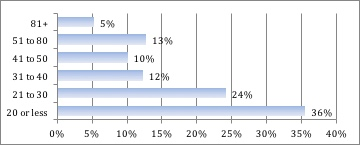
\includegraphics[width=0.7\textwidth]{plots/maxnumstudy}
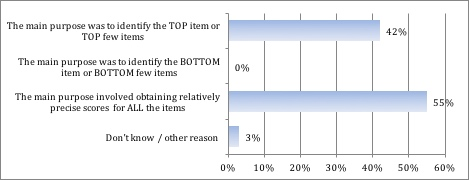
\includegraphics[width=0.7\textwidth]{plots/maxdiffpurpose}
\end{center}
\end{figure}

\subsection{Model Estimation Details}
For any individual-task combination, let $Y_{B_S}(z)$ be the binary choice variable, where $Y_{B_S}(z)$ equals 1 if the item $z \in S$ is selected as best in the set $S$ and 0 otherwise. $Y_{W_S}(z)$ is the indicator of whether item $z \in S$ is selected as worst. The design matrix $X_{B_S}$ (of size $N*J$-by-$K$) contains indicator variables taking on a value of 1 for each item in the current set $S$ faced by a respondent, and 0 otherwise. To signal the item as worst, we set $X_{W_S}=-X_{B_S}$, so $X_{W_S}$ contains values of 0 or -1. We express choice probabilities -- within each of task and each respondent -- as a multinomial logit probability vector with $|S|$ alternatives. Then we stack all $J$ tasks for all $N$ respondents into vector notation, which gives the log-likelihood expression as a matrix:
\[
\log \frac{
	\exp{\left(\begin{bmatrix}Y_B\\Y_W\end{bmatrix}\theta \right)} 
}
{ 
	\exp{\left(\begin{bmatrix}X_B\\X_W\end{bmatrix}\theta\right)}
},
\]
where the rows in the matrix represent the particular respondent-task combination, $N*J$, repeated twice (best and worst), and the columns reflect the items, $\numitems$. The parameter $\theta=\{\theta_1,\ldots,\theta_\numitems \}$ is the link between the models of best and worst choices. That common parameter vector represents the overall utility of each item $1,\ldots,\numitems$. A more positive $\theta_i$ indicates that item $i$ has a greater probability of being chosen as best; the more negative, the more likely the item will be chosen as worst. Our language about utility sometimes diverges from that used in conjoint or multi-attribute profiles. Since $X$ is an indicator, $\theta$ represents only the utility of item $i$ being included versus excluded. If $\theta_i > \theta_{i'}$, we say item $i$ is ``more preferred,'' ``more important,'' or ``better.'' 

The total sum of the log-likelihood can be written as,
\[
LL(\theta)=\sum_{n=1}^N \sum_{x \in S_{n(j)}} Y_{B_{S_{n(j)}}}(x)\log{\frac{e^{\theta_x}}{\sum_{z\in S_{n(j)}} e^{\theta_z}}}+ Y_{W_{S_{n(j)}}}(x)\log{\frac{e^{-\theta_x}}{\sum_{z\in S_{n(j)}} e^{-\theta_z}}},
\]
where $S_{n(j)}$ denotes the set from the $j$th choice task faced by respondent $n$. We then find $\theta$ that maximizes the log-likelihood. 

\section{Practical Considerations for Implementation}

% The process could be repeated to choose the five items to show in the second task for the 101st respondent, etc. This could be done with or without updating the logit parameters after recording the responses to the first task. For practical computational purposes, to reduce the load on the server managing the data collection, the model estimates would be updated only after every 20th respondent has completed the survey. 

% Another concern with using the bandit algorithm directly on the problem would be the repetitiveness of a tasks for any one respondent. If left alone, the bandit algorithm could update within each respondent, converging to a small subset of the best items. While a choices of best and worst among a set of five items may be somewhat stochastic, an real human respondent would be frustrated being shown the same or nearly identical sets of items repeatedly. To avoid this, we only allow the algorithm adapt between respondent, and then we can leverage the fully orthogonal MaxDiff design of the best $\numperset$ within each respondent.

Two practical issues should be considered when implementing Bandit MaxDiff for large-scale ranking and selection problems. 

First, we want to avoid asking extremely similar questions of the same respondent. A natural consequence of adaptive methods is convergence: As the sample size grows, certain product or service characteristics achieve high preference scores with small standard errors. Without additional restrictions, the same few items will eventually be drawn into adjacent MaxDiff tasks for the same respondent. Although this is statistically most efficient, it upsets human respondents. 

To avoid convergence, the system shows each respondent a fixed number of 20 to 30 items in a balanced, near-orthogonal design, leading to a low degree of repetition across adjacent sets. The approach is similar to Express MaxDiff \citep{wirth2012largeset}, but the 20 items selected for each respondent are adaptive, leveraging information from the previous respondents and focusing the most recent respondent's efforts on discriminating among items already judged preferential. The approach also keeps the respondent from tiring out, as he or she is not forced to address 120 items at a time.

Second, we must update the data with regular frequency. If respondents take a firm's survey sequentially, all the data from previous participants can be used to generate new surveys. Often, however, this does not occur. As an alternative, the administrator can update the data once every $b$ respondents complete the survey and then decide the questions for the next $b$ individuals. We call this batch size and in our empirical analysis let $b=20$.

Both practical considerations avoid latency during a single survey and across respondents. Since all questions for the next $b$ individuals are set, no computation takes place before or between questions during a single survey.



\section{Approximations and Practical Considerations}

%\subsection{Changing Exploration Parameters}
%Almost all of the adaptive methods have parameters for all of these methods and the trade off is robustness against heterogeneity in the respondents verses speed of convergence. All the Greatest Uncertainty with random perturbation and Misclassification Minimization with random perturbation $c=\infty$ (or any $c \geq 250$ in the case 120 items showing 20 items to each respondent) is fixed express, and using $c=0$ , $\epsilon$-greedy with $\epsilon=1$, and $\epsilon$-diffuse TS with $\epsilon=1$ and $\delta=0$ are the same sampling scheme as fixed express. Also $\epsilon$-diffuse TS with $\epsilon=0$ is regular TS.  Our recommended ranges for the different parameters are $\frac{1}{5}\leq \epsilon \leq \frac{1}{2}$, $\frac{1}{4}\leq \delta \leq \frac{1}{2}$ and $.01 \leq c \leq 1$.


% \subsection{What about Double Adaptivity?}
% In~\cite{orme2006adaptive}, one of the authors presented a paper on Adaptive MaxDiff that featured within-respondent adaptation rather than what we have shown here in Bandit MaxDiff based on Thompson Sampling, which is an across-respondent adaptive approach. For the within-respondent adaptive procedure, items that a respondent indicates are worst are dropped from further consideration by that same respondent through a round-robin tournament until eventually that respondent's best item is identified.  We thought adding this additional layer of within-respondent adaptivity on top of the Bandit MaxDiff approach could additionally lift its performance.  To our surprise, this double-adaptive approach actually performed worse than Bandit MaxDiff alone in terms of hit rates for the top 3 or 10 items for the sample.  After some head-scratching (and much code checking), we determined that the lack of improvement was due to degree of heterogeneity across the robotic respondents.  For example, if we are interviewing a respondent who doesn't agree much with the overall population regarding which are the top items, it is detrimental to allow that respondent to drop from further consideration (due to judging them worst) what actually are among the globally most preferred items.  It serves the greater good for each respondent to spend increased effort judging among the items that previous respondents on average have judged as potentially best.

\subsection{Asymptotic Distribution vs. Bayesian Bootstrap}

As an alternative to Bayesian Bootstrapping for posterior draws, we can sample from the asymptotic distribution via MLE implied by the estimated mean and standard errors, sampling $u \sim N(\theta,H^{-1})$, where $\theta$ is the minimizer of the negative log-likelihood and $H$ is the Hessian of the negative log-likelihood evaluated at $\theta$. The sampling methods perform similarly using draws from Bayesian Bootstrapping and asymptotic distribution.

Another method allows for online updates for streaming data without model estimation. MaxDiff tasks yield a number of pairwise comparisons via a single best-worst pair. We can therefore act as if the respondent states all such comparisons and assign a win to the more preferred item and loss to the others. By tallying wins for each item, we can compare win percentages among items that have faced each other and find a noisy measure of underlying utility. Taking win percentage as an average, $\hat{p}_{win}$, we can use its standard error, $se_{win}$, in TS as follows:
\begin{align}
\hat{p}_{k,win} &= n_{k,wins} / n_{trials} \\
\text{se}_{k,win} &= \sqrt{  \frac{ \hat{p}_{k,win} (1-\hat{p}_{k,win}) } {n_{trials}}.  } \\
\end{align}

The mean and variance can be used for sampling from the winning percentages distribution in TS or \edts. For TS, after sampling one $p_{k,win}^{ts}$ for each of the $k=1,\ldots,K$ items independently, we can rank order and identify the top set of values. For \edts, we do this for two different normal distributions, one with $\text{se}_{k,win}$ and one with the inflated standard error, $\delta \text{se}_{k,win}$.


\subsection{Best, Not Best-Worst}

Adaptive MaxDiff approaches perform best when the researcher is mainly interested in identifying the top few items in a set. Is it valuable in this case to ask respondents to identify the worst item within each MaxDiff set? The value of asking respondents to indicate both their best and worst choices within each set more than compensates for the 40\% additional effort we estimate the questions add to the total interview time when working with human respondents.

In a five item set (A,B,C,D, and E), we have 10 possible two-way comparisons. If we assume A is preferred to B and B is preferred to C and so on, asking respondents to indicate only the best item will let us know A$>$B, A$>$C, A$>$D, and A$>$E (4/10 comparisons). By asking about respondents' least preferred items, we also know B$>$E, C$>$E, and D$>$E (7/10 comparisons), leaving only the order relationship between B, C, and D unknown.

The case of asking for top choices when all respondents have the same preferences aligns with the marked bandit problem outlined by~\cite{simchowitz2016best}, where the authors offer different algorithms for pulling the arms and upper and lower bounds on how many queries it takes to identify the top $k$ items with high probability. 


\subsection{Sparse MaxDiff vs. Express MaxDiff}
In ~\cite{wirth2012largeset}, the authors compare non-adaptive Sparse MaxDiff and Express MaxDiff. For Fixed Sparse MaxDiff, we show each item to each respondent an equal number of times (if possible). With 120 items, 12 sets and five items per set appear on average $\frac{12*5}{120} = 0.5$ times per respondent. We compare the results using our simulation and find a modest edge in performance for Express MaxDiff---Sparse MaxDiff ending at 85.6\% for a top 10 hit rate and Express MaxDiff ending at 87.7\%.

\end{APPENDICES}

\end{document}